\documentclass[12pt,a4paper,openany]{ctexbook}
% 基础宏包
\usepackage{geometry}
\usepackage{graphicx}
\usepackage{amsmath,amssymb}
\usepackage{booktabs}
\usepackage{array}
\usepackage{multirow}
\usepackage{enumitem}
\usepackage{xcolor}
\usepackage{listings}
\usepackage{hyperref}
\usepackage{fancyhdr}
\usepackage{tikz}
\usetikzlibrary{shapes,arrows,positioning,calc,decorations.pathreplacing,mindmap,trees}

% 页面设置
\geometry{left=2.5cm,right=2.5cm,top=2.5cm,bottom=2.5cm,headheight=15pt}

% 改善排版警告
\tolerance=1000
\emergencystretch=3em
\hbadness=10000
\vbadness=10000

% 减少章节前后空白
\usepackage{titlesec}
\titlespacing*{\chapter}{0pt}{-20pt}{20pt}
\titlespacing*{\section}{0pt}{10pt}{5pt}
\titlespacing*{\subsection}{0pt}{8pt}{4pt}

% 超链接设置
\hypersetup{colorlinks=true,linkcolor=blue,urlcolor=blue}

% 代码样式
\lstset{basicstyle=\ttfamily\small,breaklines=true,frame=single,backgroundcolor=\color{gray!10}}

% 页眉页脚
\pagestyle{fancy}
\fancyhf{}
\fancyhead[L]{\leftmark}
\fancyhead[R]{\thepage}
\renewcommand{\headrulewidth}{0.4pt}

% 定义颜色盒子
\usepackage{tcolorbox}
\tcbuselibrary{skins,breakable}
\newtcolorbox{notebox}{colback=blue!5,colframe=blue!75!black,title=注意,fonttitle=\bfseries}
\newtcolorbox{tipbox}{colback=green!5,colframe=green!75!black,title=提示,fonttitle=\bfseries}
\newtcolorbox{formulabox}{colback=yellow!5,colframe=orange!75!black,title=公式,fonttitle=\bfseries}
\newtcolorbox{examplebox}[1][]{colback=gray!5,colframe=gray!75!black,title=#1,fonttitle=\bfseries}
\newtcolorbox{conceptbox}{colback=purple!5,colframe=purple!75!black,title=概念,fonttitle=\bfseries}

\title{\Huge\textbf{人工智能导论教程}}
\author{基于课程笔记整理}
\date{\today}

\begin{document}
\maketitle
\tableofcontents

% 引入各章节
%========================================
\chapter{人工智能概述}
%========================================

\section{人工智能的定义}

\subsection{基本概念}
\begin{conceptbox}
\textbf{人工智能}（Artificial Intelligence, AI）是用人工方法在机器（计算机）上实现智能，或使机器具备类人智能的学科。

\textbf{智能体}（Agent）是指能够感知环境并通过行动改变环境的实体。人也可以被看作是一种智能体。
\end{conceptbox}

人工智能是一门综合性学科，旨在构建智能机器以模拟、延伸和扩展人类智能。它融合了多个学科的理论与方法：
\begin{itemize}[leftmargin=2em,itemsep=0pt]
    \item \textbf{上层来源学科}：脑科学、认知科学、心理学、系统科学、计算机科学、控制论、信息论
    \item \textbf{核心能力}：推理、学习、规划、感知、知识获取、搜索、不确定性处理
    \item \textbf{应用方向}：博弈、定理证明、语言图像理解、机器人学、专家系统
\end{itemize}

\subsection{人工智能的分类}

\subsubsection{按功能划分（模拟人的智能）}
\begin{enumerate}[leftmargin=2em,itemsep=0pt]
    \item \textbf{感知智能}：视觉、听觉、触觉等感官能力
    \item \textbf{认知智能}：语言理解、知识推理等思维能力
    \item \textbf{创造智能}：灵感、顿悟等创新能力
\end{enumerate}

\subsubsection{按层次划分（从弱到强）}
\begin{table}[htbp]
\centering\small
\begin{tabular}{lll}
\toprule
\textbf{类型} & \textbf{特点} & \textbf{示例} \\
\midrule
弱人工智能 & 特定场景下的任务型AI & 语音助手、推荐系统 \\
通用人工智能(AGI) & 能处理人类水平的任务，具备持续学习能力 & 尚未实现 \\
超级人工智能 & 比人类更聪明 & 理论概念 \\
\bottomrule
\end{tabular}
\end{table}

\begin{tipbox}
\textbf{记忆口诀}：
\begin{itemize}[itemsep=0pt]
    \item "三智"：感知、认知、创造 → 模拟人类智能
    \item "三阶"：弱AI → AGI → 超级AI → 层次递进
\end{itemize}
\end{tipbox}


\section{智能体（Intelligent Agent）}

\subsection{智能体与环境}

\begin{conceptbox}
\textbf{智能体}（Agent）是指能够通过\textbf{传感器}（Sensors）感知环境，并通过\textbf{执行器}（Actuators）对环境产生作用的实体。
\end{conceptbox}

\textbf{PEAS模型}：描述智能体任务环境的四个维度：

\subsection{智能体的结构类型}

\begin{enumerate}[leftmargin=2em,itemsep=0pt]
    \item \textbf{简单反射型智能体}：基于当前感知直接做出反应（Condition-Action规则），不考虑历史。
    \begin{itemize}
        \item 例如：如果是红灯，则停车。
    \end{itemize}
    \item \textbf{基于模型的反射型智能体}：内部维护一个关于世界的\textbf{模型}（状态），用于处理部分可观察环境。
    \item \textbf{基于目标的智能体}：行动是为了达成特定\textbf{目标}（Goal），需要规划。
    \item \textbf{基于效用的智能体}：行动是为了最大化\textbf{效用}（Utility），即不仅要达成目标，还要"更快乐/更高效"。
\end{enumerate}

\subsection{BDI模型}
一种典型的理性Agent理论模型：
\begin{itemize}[leftmargin=2em,itemsep=0pt]
    \item \textbf{Belief}（信念）：Agent对环境的认知（我知道什么）。
    \item \textbf{Desire}（愿望）：Agent想达成的状态（我想做什么）。
    \item \textbf{Intention}（意图）：Agent决定去执行的行动计划（我决定做什么）。
\end{itemize}

\section{人工智能的发展历程}

\subsection{发展阶段}
\begin{table}[htbp]
\centering\small
\begin{tabular}{lll}
\toprule
\textbf{阶段} & \textbf{时间} & \textbf{特征} \\
\midrule
孕育期 & 1956年前 & 图灵测试提出、逻辑推理雏形 \\
形成期 & 1956--1969 & "人工智能"概念诞生，早期突破 \\
知识应用期 & 1970--1989 & 专家系统兴起，应用于医疗、化学等领域 \\
学派融合期 & 1990--2000 & 不同学派融合，技术逐步成熟 \\
智能科学兴起 & 2000年后 & 神经网络、深度学习爆发 \\
\bottomrule
\end{tabular}
\end{table}

\subsection{重要里程碑}
\begin{itemize}[leftmargin=2em,itemsep=0pt]
    \item \textbf{1950年}：图灵提出"图灵测试"
    \item \textbf{1956年}：达特茅斯会议正式提出"人工智能"概念
    \item \textbf{1982年}：专家系统R1投入商业使用
    \item \textbf{1997年}：深蓝战胜国际象棋世界冠军卡斯帕罗夫
    \item \textbf{2016年}：AlphaGo击败围棋世界冠军李世石
    \item \textbf{2018年}：Apollo无人驾驶上路测试
\end{itemize}

\begin{notebox}
AI经历了"高潮—低谷—复兴"的周期性发展，近年来因大数据和算力提升迎来爆发式增长。
\end{notebox}

\section{人工智能的研究学派}

\subsection{三大主流学派}

\begin{center}
\begin{tikzpicture}[
    level 1/.style={sibling distance=5cm,level distance=1.5cm},
    every node/.style={draw,rounded corners,minimum height=0.6cm,font=\small}
]
\node {人工智能学派}
    child {node[fill=red!10] {符号主义}}
    child {node[fill=green!10] {连接主义}}
    child {node[fill=blue!10] {行为主义}};
\end{tikzpicture}
\end{center}

\subsubsection{符号主义（Symbolicism）}
\begin{itemize}[leftmargin=2em,itemsep=0pt]
    \item \textbf{别名}：逻辑主义、计算机学派
    \item \textbf{原理}：基于符号操作和逻辑推理
    \item \textbf{代表}：规则引擎、知识图谱、专家系统
\end{itemize}

\subsubsection{连接主义（Connectionism）}
\begin{itemize}[leftmargin=2em,itemsep=0pt]
    \item \textbf{别名}：仿生学派、神经网络学派
    \item \textbf{原理}：模仿人脑神经元连接机制，通过训练学习模式
    \item \textbf{代表}：深度学习、CNN、RNN、Transformer
\end{itemize}

\subsubsection{行为主义（Actionism）}
\begin{itemize}[leftmargin=2em,itemsep=0pt]
    \item \textbf{别名}：进化主义、控制论学派
    \item \textbf{原理}：强调"感知—动作"闭环，注重环境交互
    \item \textbf{代表}：强化学习、机器人自主导航
\end{itemize}

\begin{tipbox}
三大学派分别对应"思维模拟"、"生物模拟"、"行为模拟"，共同推动AI演进。当前主流是连接主义（深度学习），但符号主义仍在知识工程中发挥重要作用。
\end{tipbox}

\section{人工智能的基本研究内容}

\subsection{六大核心研究方向}
\begin{enumerate}[leftmargin=2em,itemsep=0pt]
    \item \textbf{知识表示}：如何存储知识？如语义网络、本体、框架
    \item \textbf{知识推理}：如何从已知推出未知？如演绎推理、归纳推理
    \item \textbf{知识应用}：如何利用知识解决问题？如专家系统
    \item \textbf{机器学习}：让机器自动学习规律
    \item \textbf{机器感知}：视觉、听觉等输入处理
    \item \textbf{机器思维与行为}：决策、规划、行动
\end{enumerate}

\section{人工智能的应用领域}

\begin{table}[htbp]
\centering\small
\begin{tabular}{ll}
\toprule
\textbf{应用领域} & \textbf{说明} \\
\midrule
自动定理证明 & 形式化推理验证 \\
问题求解与博弈 & 国际象棋、围棋等 \\
专家系统 & 医疗诊断、故障排查 \\
模式识别 & 人脸识别、指纹识别 \\
机器视觉 & 图像识别、自动驾驶 \\
自然语言处理 & 翻译、语音助手、ChatGPT \\
人工神经网络 & 深度学习模型 \\
分布式AI与多Agent系统 & 协同智能体 \\
\bottomrule
\end{tabular}
\end{table}

\begin{examplebox}[案例分析]
\textbf{AlphaGo} = 连接主义 + 机器学习 + 博弈

\textbf{Siri/小爱同学} = 自然语言处理 + 语音识别 + 专家系统

\textbf{ChatGPT} = 深度学习 + 自然语言处理 + 强化学习
\end{examplebox}

\section{图灵测试}

\begin{conceptbox}
\textbf{图灵测试}是判断机器是否具备智能的实验方法，由图灵于1950年提出。实验由三个封闭房间组成，分别放置主持人、参与人和机器。主持人通过提问来判断谁是人、谁是机器。如果主持人无法区分，则认为该机器具备智能。
\end{conceptbox}

\begin{examplebox}[例题1.1 图灵测试]
\textbf{问题}：什么是"图灵测试"？简单描述之。
\tcblower
\textbf{答}：图灵测试是为了判断一台机器是否具备智能的实验。实验由三个封闭的房间组成，分别放置主持人、参与人和机器。主持人向参与人和机器提问，通过提问的结果来判断谁是人，谁是机器。如果主持人无法判断谁是人、谁是机器，则这台机器具备智能，即所谓的"智能机器"。
\end{examplebox}

\section{习题与解答}

\subsection{是非题}

\begin{enumerate}[leftmargin=2em,itemsep=2pt]
    \item 智能机器人的智能已经达到人类智能的水平。（×）
    \item 人也可以作为Agent。（√）
    \item 人工智能是1956年在美国达特茅斯会议上诞生的，由McCarthy教授提出"人工智能"这一术语。（√）
\end{enumerate}

\subsection{填空题}

\begin{enumerate}[leftmargin=2em,itemsep=2pt]
    \item 人工智能的研究途径有\underline{心理模拟}、\underline{生理模拟}和\underline{行为模拟}。
    \item 人工智能的基本技术包括\underline{搜索技术}、\underline{推理技术}、\underline{知识表示和知识库技术}、\underline{归纳技术}、\underline{联想技术}。
    \item 人工智能主要有\underline{博弈}、\underline{专家系统}和\underline{机器语言处理}等研究领域。
    \item 人工智能三大学派是\underline{符号主义}、\underline{联结主义}、\underline{行为主义}。
    \item AI的英文全称是\underline{Artificial Intelligence}。
    \item 人工智能的远期目标是\underline{制造智能机器}，近期目标是\underline{实现机器智能}。
\end{enumerate}

\subsection{选择题}

\begin{examplebox}[选择题1.1]
\textbf{问题}：人工智能的含义最早由一位科学家于1950年提出，并且同时提出一个机器智能的测试模型，请问这个科学家是（\quad）

A. 明斯基 \quad B. 扎德 \quad C. 图灵 \quad D. 冯·诺依曼
\tcblower
\textbf{答案}：C

图灵于1950年提出了著名的"图灵测试"，用于判断机器是否具有智能。
\end{examplebox}

\begin{examplebox}[选择题1.2]
\textbf{问题}：基于"有限合理性原理"和"物理符号系统假设"的人工智能学派一般指的是（\quad）

A. 符号主义 \quad B. 联结主义 \quad C. 行为主义
\tcblower
\textbf{答案}：A

符号主义基于物理符号系统假设，认为智能可以通过符号操作和逻辑推理来实现。
\end{examplebox}

\begin{examplebox}[选择题1.3]
\textbf{问题}：神经网络研究属于下列哪个学派？（\quad）

A. 符号主义 \quad B. 连接主义 \quad C. 行为主义 \quad D. 都不是
\tcblower
\textbf{答案}：B

神经网络模仿人脑神经元的连接机制，属于连接主义（仿生学派）。
\end{examplebox}

\begin{examplebox}[选择题1.4]
\textbf{问题}：1997年5月，著名的"人机大战"，最终计算机以3.5比2.5的总比分将世界国际象棋棋王卡斯帕罗夫击败，这台计算机被称为（\quad）

A. 深蓝 \quad B. IBM \quad C. 深思 \quad D. 蓝天
\tcblower
\textbf{答案}：A

IBM的"深蓝"（Deep Blue）是第一个在标准比赛时限内击败国际象棋世界冠军的计算机系统。
\end{examplebox}

\begin{examplebox}[选择题1.5]
\textbf{问题}：下列哪个不是人工智能的研究领域？（\quad）

A. 机器证明 \quad B. 模式识别 \quad C. 人工生命 \quad D. 编译原理
\tcblower
\textbf{答案}：D

编译原理是计算机科学的基础学科，不属于人工智能的研究领域。
\end{examplebox}

\subsection{简答题}

\begin{examplebox}[简答题1.1]
\textbf{问题}：什么是人工智能？人工智能与传统计算机程序的区别是什么？
\tcblower
\textbf{答}：人工智能是研究如何制造人造的智能机器或智能系统来模拟人类智能活动的能力，以延伸人类智能的科学。

人工智能程序与传统计算机程序的区别：
\begin{enumerate}[itemsep=0pt]
    \item AI以符号表示的知识为研究对象，而不是以数值数据为研究对象
    \item AI采用启发式搜索方法，而不是普通的算法
    \item AI中控制结构与知识是分离的
    \item AI允许出现不正确的答案
\end{enumerate}
\end{examplebox}

\begin{examplebox}[简答题1.2]
\textbf{问题}：人工智能主要有哪几种研究途径和技术方法？简单说明之。
\tcblower
\textbf{答}：
\begin{enumerate}[itemsep=0pt]
    \item \textbf{符号智能}：主要以符号知识为基础，通过符号推理进行问题求解而实现的智能，主要包括知识工程和符号处理技术
    \item \textbf{计算智能}：是以数据计算为基础，通过数值计算进行问题求解而实现的智能，包括人工神经网络、进化计算、模糊技术等
\end{enumerate}
\end{examplebox}

\section{本章小结}

本章介绍了人工智能的基本概念：
\begin{itemize}[leftmargin=2em,itemsep=0pt]
    \item AI的定义：用人工方法在机器上实现智能
    \item AI的分类：按功能分（感知/认知/创造）、按层次分（弱AI/AGI/超级AI）
    \item AI的发展历程：四个阶段 + 关键里程碑事件
    \item AI的三大学派：符号主义、连接主义、行为主义
    \item AI的研究内容：知识表示、推理、学习、感知、思维、行为
    \item AI的应用领域：NLP、CV、机器人、专家系统、博弈等
    \item 图灵测试：判断机器智能的经典方法
\end{itemize}

\textbf{重点掌握}：
\begin{itemize}[leftmargin=2em,itemsep=0pt]
    \item 三大学派的区别与联系
    \item 发展历程中的重要时间节点
    \item AI的分类方式
    \item 图灵测试的概念和意义
\end{itemize}

%========================================
\chapter{知识表示}
%========================================

\section{知识的基本概念}

\subsection{知识的定义}
\begin{conceptbox}
\textbf{知识}是信息之间关联的结果，最常见的是用"如果……，则……"来表达因果关系。
\end{conceptbox}

在AI中，知识分为两类：
\begin{itemize}[leftmargin=2em,itemsep=0pt]
    \item \textbf{事实（Fact）}：对客观世界的描述，如"蚂蚁搬家"
    \item \textbf{规则（Rule）}：事物间的因果关系，如"如果蚂蚁搬家，则大雨将至"
\end{itemize}

\subsection{知识的特性}
\begin{table}[htbp]
\centering\small
\begin{tabular}{ll}
\toprule
\textbf{特性} & \textbf{解释} \\
\midrule
相对正确性 & 在特定条件下成立，可能随环境变化而失效 \\
不确定性 & 很多知识存在概率或模糊性 \\
可表示性 & 可以用某种语言或形式化方法表达 \\
可利用性 & 能被计算机存储、处理并用于推理决策 \\
\bottomrule
\end{tabular}
\end{table}

\begin{notebox}
知识不是绝对真理，而是人类对客观世界的认识结晶。例如："水在0°C结冰"的前提是标准大气压下。
\end{notebox}

\section{命题逻辑}

\subsection{命题的定义}
\begin{conceptbox}
\textbf{命题（Proposition）}是一个非真即假的陈述句，具有唯一的真值（T或F）。
\end{conceptbox}

\textbf{判断是否为命题的标准}：
\begin{enumerate}[leftmargin=2em,itemsep=0pt]
    \item 是否为陈述句？
    \item 是否有唯一真值（T或F）？
\end{enumerate}

\textbf{非命题的例子}：
\begin{itemize}[leftmargin=2em,itemsep=0pt]
    \item "你吃饭了吗？" —— 疑问句，无真假
    \item "哇！好美！" —— 感叹句，无明确真值
\end{itemize}

\subsection{逻辑连接词}
使用连接词将简单命题组合成复杂命题：

\begin{table}[htbp]
\centering\small
\begin{tabular}{ccl}
\toprule
\textbf{连接词} & \textbf{符号} & \textbf{含义} \\
\midrule
非 & $\neg P$ & P不成立 \\
与 & $P \land Q$ & P和Q都为真 \\
或 & $P \lor Q$ & P或Q至少一个为真 \\
蕴含 & $P \to Q$ & 如果P为真，则Q必须为真 \\
等价 & $P \leftrightarrow Q$ & P和Q同真或同假 \\
\bottomrule
\end{tabular}
\end{table}

\subsection{真值表}
\begin{table}[htbp]
\centering\small
\begin{tabular}{cc|ccccc}
\toprule
$P$ & $Q$ & $\neg P$ & $P \land Q$ & $P \lor Q$ & $P \to Q$ & $P \leftrightarrow Q$ \\
\midrule
T & T & F & T & T & T & T \\
T & F & F & F & T & F & F \\
F & T & T & F & T & T & F \\
F & F & T & F & F & T & T \\
\bottomrule
\end{tabular}
\end{table}

\begin{notebox}
\textbf{特别注意}：$P \to Q$ 在P为假时恒为真（即使Q为假），这称为"空真"。
\end{notebox}

\section{谓词逻辑}

\subsection{谓词与量词}
谓词逻辑使用变量、谓词、量词表示更复杂的知识。

\textbf{量词}：
\begin{itemize}[leftmargin=2em,itemsep=0pt]
    \item \textbf{全称量词} $\forall$：表示"所有"
    \item \textbf{存在量词} $\exists$：表示"存在"
\end{itemize}

\subsection{量词组合示例}
设谓词 $F(x, y)$ 表示"x和y是朋友"：

\begin{table}[htbp]
\centering\small
\begin{tabular}{ll}
\toprule
\textbf{公式} & \textbf{含义} \\
\midrule
$(\forall x)(\forall y)F(x,y)$ & 所有人都是彼此的朋友 \\
$(\forall x)(\exists y)F(x,y)$ & 每个人都有至少一个朋友 \\
$(\exists x)(\exists y)F(x,y)$ & 至少有两个人是朋友 \\
$(\exists x)(\forall y)F(x,y)$ & 存在一个人和所有人都是朋友 \\
\bottomrule
\end{tabular}
\end{table}

\subsection{辖域与变元}
\begin{itemize}[leftmargin=2em,itemsep=0pt]
    \item \textbf{辖域（Scope）}：量词后面被作用的部分
    \item \textbf{约束变元}：出现在量词辖域内的同名变量
    \item \textbf{自由变元}：未被任何量词约束的变量
\end{itemize}

\subsection{常见等价式}
\begin{formulabox}
\textbf{德摩根律}：
\begin{align*}
\neg(P \lor Q) &\Leftrightarrow \neg P \land \neg Q \\
\neg(P \land Q) &\Leftrightarrow \neg P \lor \neg Q
\end{align*}

\textbf{量词转换}：
\begin{align*}
\neg(\exists x)P &\Leftrightarrow (\forall x)(\neg P) \\
\neg(\forall x)P &\Leftrightarrow (\exists x)(\neg P)
\end{align*}
\end{formulabox}

\section{状态空间法}

\subsection{状态空间的定义}
\begin{conceptbox}
\textbf{状态空间}是一个图，用来表示某个问题所有可能的状态及其之间的关系，可记为四元组：$(S, O, s_0, G)$
\end{conceptbox}

\begin{itemize}[leftmargin=2em,itemsep=0pt]
    \item $S$：所有可能的状态集合
    \item $O$：操作符集合（状态转换操作）
    \item $s_0$：初始状态集合
    \item $G$：目标状态集合
\end{itemize}

\subsection{状态空间图}
\begin{center}
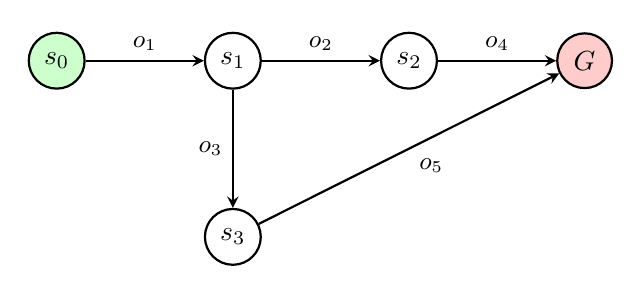
\begin{tikzpicture}[node distance=1.5cm,>=stealth,thick]
\node[draw,circle,fill=green!20] (s0) {$s_0$};
\node[draw,circle,right=of s0] (s1) {$s_1$};
\node[draw,circle,right=of s1] (s2) {$s_2$};
\node[draw,circle,below=of s1] (s3) {$s_3$};
\node[draw,circle,right=of s2,fill=red!20] (G) {$G$};

\draw[->] (s0) -- node[above]{\small $o_1$} (s1);
\draw[->] (s1) -- node[above]{\small $o_2$} (s2);
\draw[->] (s1) -- node[left]{\small $o_3$} (s3);
\draw[->] (s2) -- node[above]{\small $o_4$} (G);
\draw[->] (s3) -- node[below right]{\small $o_5$} (G);
\end{tikzpicture}
\end{center}

\textbf{求解路径}：从初始状态$s_0$到目标状态$G$的一条路径，路径上的操作序列就是问题的解。

\section{产生式系统}

\subsection{产生式的基本形式}

\subsubsection{确定性规则}
\begin{lstlisting}
IF P THEN Q
\end{lstlisting}
或符号形式：$P \to Q$

\begin{itemize}[leftmargin=2em,itemsep=0pt]
    \item $P$：前提（前项），条件满足时才能触发
    \item $Q$：结论（后项），当P成立时应得出的结果
\end{itemize}

\subsubsection{不确定性规则}
\begin{lstlisting}
IF P THEN Q (置信度)
\end{lstlisting}

例如：\texttt{IF 头痛 AND 流鼻涕 THEN 感冒 (0.8)}

表示有80\%的可能性是感冒。

\subsection{产生式系统的组成}
\begin{center}
\begin{tikzpicture}[node distance=2cm,>=stealth,thick]
\node[draw,rectangle,minimum width=3cm,minimum height=1cm,fill=blue!10] (rule) {规则库};
\node[draw,rectangle,minimum width=3cm,minimum height=1cm,right=of rule,fill=green!10] (engine) {推理机};
\node[draw,rectangle,minimum width=3cm,minimum height=1cm,right=of engine,fill=yellow!10] (db) {综合数据库};

\draw[<->] (rule) -- (engine);
\draw[<->] (engine) -- (db);
\end{tikzpicture}
\end{center}

\begin{table}[htbp]
\centering\small
\begin{tabular}{ll}
\toprule
\textbf{组成部分} & \textbf{功能} \\
\midrule
规则库 & 存储所有产生式规则 \\
推理机 & 控制规则匹配与执行过程 \\
综合数据库 & 存放当前已知的事实、中间结果和最终结论 \\
\bottomrule
\end{tabular}
\end{table}

\subsection{求解步骤}
\begin{enumerate}[leftmargin=2em,itemsep=0pt]
    \item 初始化综合数据库（输入初始事实）
    \item 建立规则库
    \item 匹配规则（检查是否有规则的前提与当前事实匹配）
    \item 执行规则（将结论加入数据库）
    \item 检查是否已得解
    \item 若无可用规则，请求用户提供更多信息
    \item 终止求解
\end{enumerate}

\begin{examplebox}[例题2.1 产生式推理]
\textbf{题目}：已知字符A和B，目标得到字符F。规则如下：
\begin{itemize}[itemsep=0pt]
    \item $R_1$: $A \land B \to C$
    \item $R_2$: $A \land C \to D$
    \item $R_3$: $B \land C \to G$
    \item $R_4$: $B \land E \to F$
    \item $R_5$: $D \to E$
\end{itemize}
\tcblower
\textbf{解答}：
\begin{enumerate}[itemsep=0pt]
    \item 初始事实：A, B
    \item 应用$R_1$：$A \land B \to C$ → 得到C
    \item 应用$R_2$：$A \land C \to D$ → 得到D
    \item 应用$R_5$：$D \to E$ → 得到E
    \item 应用$R_4$：$B \land E \to F$ → 得到F ✓
\end{enumerate}
\textbf{推理路径}：$A,B \to C \to D \to E \to F$
\end{examplebox}

\section{语义网络}

\subsection{基本概念}
\begin{conceptbox}
\textbf{语义网络}是一种用带标识的有向图来表示知识的方法，由节点和弧组成。
\end{conceptbox}

\begin{itemize}[leftmargin=2em,itemsep=0pt]
    \item \textbf{节点（Node）}：表示概念、对象、事件、属性等
    \item \textbf{弧（Arc）}：表示节点间的语义关系
\end{itemize}

\subsection{基本语义关系}

\subsubsection{类属关系}
\begin{table}[htbp]
\centering\small
\begin{tabular}{lll}
\toprule
\textbf{关系} & \textbf{含义} & \textbf{示例} \\
\midrule
ISA & 实例关系：A是B的一个实例 & 鹦鹉 → ISA → 鸟 \\
AMO & 成员关系：A是B的成员 & 李琦 → AMO → 学生会 \\
AKO & 种类关系：A是B的一种类型 & 鸟 → AKO → 动物 \\
\bottomrule
\end{tabular}
\end{table}

\subsubsection{包含关系（聚集关系）}
\begin{itemize}[leftmargin=2em,itemsep=0pt]
    \item \textbf{Part-of}：某物是另一物的一部分
    \item 例如：轮胎 → Part-of → 汽车
    \item \textbf{特点}：不具备属性继承性
\end{itemize}

\subsubsection{属性关系}
\begin{itemize}[leftmargin=2em,itemsep=0pt]
    \item \textbf{Have}：具备某种属性（鸟 → Have → 翅膀）
    \item \textbf{Can}：能够做某事（洗衣机 → Can → 洗衣服）
\end{itemize}

\subsubsection{其他关系}
\begin{itemize}[leftmargin=2em,itemsep=0pt]
    \item \textbf{时间关系}：Before、After
    \item \textbf{位置关系}：Located-at、Located-in
    \item \textbf{因果关系}：If-then
    \item \textbf{相近关系}：Similar-to
\end{itemize}

\subsection{语义网络示例}
\begin{center}
\begin{tikzpicture}[node distance=2cm,>=stealth,thick]
\node[draw,ellipse] (animal) {动物};
\node[draw,ellipse,below left=of animal] (mammal) {哺乳动物};
\node[draw,ellipse,below=of mammal] (cat) {猫};
\node[draw,ellipse,below=of cat] (sphinx) {斯芬克斯猫};
\node[draw,rectangle,right=of sphinx] (fur) {毛};

\draw[->] (mammal) -- node[left]{\small AKO} (animal);
\draw[->] (cat) -- node[left]{\small AKO} (mammal);
\draw[->] (sphinx) -- node[left]{\small ISA} (cat);
\draw[->,dashed] (sphinx) -- node[above]{\small Not-Have} (fur);
\end{tikzpicture}
\end{center}

\begin{notebox}
\textbf{属性继承}：类属关系（ISA、AKO）支持属性继承，包含关系（Part-of）不支持。
\end{notebox}

\begin{notebox}
\textbf{属性继承}：类属关系（ISA、AKO）支持属性继承，包含关系（Part-of）不支持。
\end{notebox}

\subsection{语义网络的推理}

基于语义网络的推理主要有以下三种方式：

\begin{enumerate}[leftmargin=2em,itemsep=0pt]
    \item \textbf{网络匹配（Matching）}
    \begin{itemize}
        \item 在知识库的语义网络中寻找与待求解问题相匹配的片段。
        \item 如果找到匹配的片段，则问题得到解答。
    \end{itemize}
    
    \item \textbf{网络继承（Inheritance）}
    \begin{itemize}
        \item 利用ISA和AKO链，下层节点自动拥有上层节点的属性。
        \item 这是一个\textbf{默认推理}过程，除非有明确的特例（如鸵鸟是鸟，但不会飞）。
    \end{itemize}
    
    \item \textbf{网络演绎（Deduction）}
    \begin{itemize}
        \item 根据语义网络中的隐含关系（如传递性）推导出新的关系。
        \item 例如：A是B的一部分，B是C的一部分 $\to$ A是C的一部分。
    \end{itemize}
\end{enumerate}

\section{框架表示法}

\subsection{框架的结构}
\begin{conceptbox}
\textbf{框架（Frame）}是一种描述对象属性的数据结构，由若干个槽（Slot）组成，每个槽又可划分为若干个侧面（Facet）。
\end{conceptbox}

\begin{table}[htbp]
\centering\small
\begin{tabular}{ll}
\toprule
\textbf{术语} & \textbf{含义} \\
\midrule
框架（Frame） & 描述某一类事物的整体结构 \\
槽（Slot） & 表示对象的一个属性 \\
侧面（Facet） & 描述槽的某个方面（如默认值、约束） \\
槽值 & 槽的具体取值 \\
\bottomrule
\end{tabular}
\end{table}

\subsection{框架表示步骤}
\begin{enumerate}[leftmargin=2em,itemsep=0pt]
    \item 分析待表示知识中的对象及其属性，设置框架中的槽
    \item 考察各对象间的联系，使用槽名描述上下层框架间的关系
    \item 对各层对象的槽和侧面进行合理组织，避免信息重复
\end{enumerate}

\begin{examplebox}[例题2.2 框架表示]
\textbf{题目}：用框架表示以下新闻：

"今天，一次强度为里氏8.5级的强烈地震袭击了下斯洛文尼亚地区，造成25人死亡和5亿美元的财产损失。"
\tcblower
\textbf{解答}：
\begin{lstlisting}
框架名：<地震3>
  ISA: <地震>
  地点: 下斯洛文尼亚
  时间: 今天
  震级: 8.5
  伤亡人数: 25
  财产损失: 5亿美元
\end{lstlisting}
\end{examplebox}

\section{专家系统的结构与原理}

\begin{conceptbox}
\textbf{专家系统}（Expert System）是一种智能计算机程序，能够利用人类专家的知识和推理方法来解决特定领域中的复杂问题。
\end{conceptbox}

\subsection{六大核心组件}

专家系统通常由以下六个部分组成：

\begin{enumerate}[leftmargin=2em,itemsep=0pt]
    \item \textbf{知识库（Knowledge Base）}
    \begin{itemize}
        \item 存储特定领域的专业知识（事实、规则等）。
        \item 是专家系统的核心，其质量决定系统的性能。
    \end{itemize}
    
    \item \textbf{推理机（Inference Engine）}
    \begin{itemize}
        \item 根据当前已知事实，利用知识库中的知识进行推理。
        \item 常用推理策略：正向推理、反向推理、混合推理。
    \end{itemize}
    
    \item \textbf{综合数据库（Global Database）}
    \begin{itemize}
        \item 又称动态数据库或黑板，用于存放初始证据、中间结果和最终结论。
    \end{itemize}
    
    \item \textbf{人机界面（User Interface）}
    \begin{itemize}
        \item 用户与系统交互的窗口，负责接受用户输入和输出系统解答。
    \end{itemize}
    
    \item \textbf{解释模块（Explanation Module）}
    \begin{itemize}
        \item "Why"解释：为什么系统问这个问题？
        \item "How"解释：系统是如何得出这个结论的？
        \item 增强用户对系统的信任感。
    \end{itemize}
    
    \item \textbf{知识获取模块（Knowledge Acquisition）}
    \begin{itemize}
        \item 负责将人类专家的知识转化为计算机可表示的形式并存入知识库。
        \item 是构建专家系统的"瓶颈"环节。
    \end{itemize}
\end{enumerate}

\subsection{先进专家系统的特点}

随着技术发展，新一代（先进）专家系统表现出以下特征：
\begin{itemize}[leftmargin=2em,itemsep=0pt]
    \item \textbf{并行分布式处理}：多专家协同工作。
    \item \textbf{多专家协同}：解决单一领域知识的局限性。
    \item \textbf{自学习能力}：能从经验中学习新知识。
    \item \textbf{深层知识推理}：不仅基于浅层经验规则，还能进行基于模型的深层推理。
\end{itemize}

\section{习题与解答}

\subsection{是非题}

\begin{enumerate}[leftmargin=2em,itemsep=2pt]
    \item 语义网络是一种有向图，它有5个级别，7种类型。（√）
    \item 单位关系不在语义网络表示的范围内。（×）
    \item 对象与类是实例关系。（√）
    \item 基于语义网络的推理主要有网络匹配、网络继承和网络演绎三种方式。（√）
    \item 对"与"、"或"、"蕴含"关系，在语义网络表示时主要加上"与"、"或"、"蕴含"结点。（√）
    \item 框架之间也有从属关系、实例关系等。（√）
    \item 命题是可以判断真假的陈述句。（√）
\end{enumerate}

\subsection{填空题}

\begin{enumerate}[leftmargin=2em,itemsep=2pt]
    \item 在人工智能中，通常知识有\underline{谓词逻辑表示法}、\underline{产生式系统表示法}、\underline{语义网络表示法}、\underline{框架表示法}等表示的方法。
    \item 产生式系统包括\underline{知识库}和\underline{推理机}，知识库由\underline{规则库}和\underline{数据库}组成。
    \item 产生式系统的推理可分为\underline{正向推理}、\underline{反向推理}和\underline{混合推理}。
    \item 语义网络是用\underline{有向图}方法表示的，由\underline{节点}和\underline{弧}二元组构成。其中节点表示概念、属性、事件等；弧表示节点间的语义关系。
    \item 在语义网络中，为了表示节点间属性的继承推理，规定了两个约定俗成的链，命名为\underline{ISA}和\underline{AKO}，用来表明类和子类、类和个体之间的关系。
    \item 仅个体变元被量化的谓词称为\underline{一阶谓词}。
    \item 在谓词公式中，紧接于量词之后被量词作用的谓词公式称为该量词的\underline{辖域}，而在一个量词的辖域中与该量词的指导变元相同的变元称为\underline{约束变元}，其他变元称为\underline{自由变元}。
\end{enumerate}

\subsection{选择题}

\begin{examplebox}[选择题2.1]
\textbf{问题}：语义网络表达知识时，有向弧AKO链、ISA链是用来表达节点知识的（\quad）

A. 无序性 \quad B. 可扩充性 \quad C. 继承性
\tcblower
\textbf{答案}：C

AKO（A Kind Of）和ISA（Is A）链用于表示类属关系，支持属性的继承推理。
\end{examplebox}

\begin{examplebox}[选择题2.2]
\textbf{问题}：从已知事实出发，通过规则库求得结论的产生式系统的推理方式是（\quad）

A. 正向推理 \quad B. 反向推理 \quad C. 双向推理
\tcblower
\textbf{答案}：A

正向推理（数据驱动）从已知事实出发，逐步应用规则得出结论。反向推理（目标驱动）从目标出发，寻找支持目标的事实。
\end{examplebox}

\subsection{语义网络表示例题}

\begin{examplebox}[例题2.3 语义网络表示人物关系]
\textbf{问题}：用语义网络表示"胡涛是创新公司的经理，他35岁，住在飞天胡同68号"。
\tcblower
\begin{center}
\begin{tikzpicture}[node distance=2cm,>=stealth,thick]
\node[draw,ellipse] (hutao) {胡涛};
\node[draw,ellipse,right=of hutao] (company) {创新公司};
\node[draw,rectangle,above=1.5cm of hutao] (age) {35};
\node[draw,rectangle,below=1.5cm of hutao] (addr) {飞天胡同68号};
\node[draw,ellipse,right=of company] (manager) {经理};

\draw[->] (hutao) -- node[above]{\small 工作于} (company);
\draw[->] (hutao) -- node[left]{\small 年龄} (age);
\draw[->] (hutao) -- node[left]{\small 住于} (addr);
\draw[->] (hutao) -- node[below]{\small ISA} (manager);
\end{tikzpicture}
\end{center}
\end{examplebox}

\begin{examplebox}[例题2.4 语义网络表示事件]
\textbf{问题}：用语义网络表示"高老师从3月到7月给计算机系学生讲《计算机网络》课"。
\tcblower
\begin{center}
\begin{tikzpicture}[node distance=1.8cm,>=stealth,thick]
\node[draw,ellipse,fill=yellow!20] (event) {讲课事件};
\node[draw,ellipse,left=of event] (teacher) {高老师};
\node[draw,ellipse,right=of event] (student) {计算机系学生};
\node[draw,rectangle,above=of event] (course) {计算机网络};
\node[draw,rectangle,below left=1.2cm of event] (start) {3月};
\node[draw,rectangle,below right=1.2cm of event] (end) {7月};

\draw[->] (teacher) -- node[above]{\small 主体} (event);
\draw[->] (event) -- node[above]{\small 对象} (student);
\draw[->] (event) -- node[left]{\small 课程} (course);
\draw[->] (event) -- node[below left]{\small 开始} (start);
\draw[->] (event) -- node[below right]{\small 结束} (end);
\end{tikzpicture}
\end{center}
\end{examplebox}

\begin{examplebox}[例题2.5 语义网络表示层次关系]
\textbf{问题}：用语义网络表示以下知识：
\begin{enumerate}[itemsep=0pt]
    \item 树和草都是植物
    \item 树和草都有根和叶
    \item 水草是草，且长在水中
    \item 果树是树，且会结果
    \item 苹果树是一种果树，它结苹果
\end{enumerate}
\tcblower
\begin{center}
\begin{tikzpicture}[node distance=1.5cm,>=stealth,thick,scale=0.9,transform shape]
\node[draw,ellipse] (plant) {植物};
\node[draw,ellipse,below left=of plant] (tree) {树};
\node[draw,ellipse,below right=of plant] (grass) {草};
\node[draw,ellipse,below=of tree] (fruit) {果树};
\node[draw,ellipse,below=of grass] (water) {水草};
\node[draw,ellipse,below=of fruit] (apple) {苹果树};
\node[draw,rectangle,right=2cm of plant] (root) {根};
\node[draw,rectangle,right=of root] (leaf) {叶};

\draw[->] (tree) -- node[left]{\small AKO} (plant);
\draw[->] (grass) -- node[right]{\small AKO} (plant);
\draw[->] (fruit) -- node[left]{\small AKO} (tree);
\draw[->] (water) -- node[right]{\small AKO} (grass);
\draw[->] (apple) -- node[left]{\small ISA} (fruit);
\draw[->] (plant) -- node[above]{\small Have} (root);
\draw[->] (plant) -- node[above]{\small Have} (leaf);
\draw[->] (fruit) -- node[right]{\small Can} ++(1.5,0) node[right]{结果};
\draw[->] (water) -- node[right]{\small 生长于} ++(1.5,0) node[right]{水中};
\draw[->] (apple) -- node[right]{\small 结} ++(1.5,0) node[right]{苹果};
\end{tikzpicture}
\end{center}
\end{examplebox}

\subsection{框架表示例题}

\begin{examplebox}[例题2.6 框架表示灾害事件]
\textbf{问题}：用框架表示以下新闻：

"新华社3月16日电：昨日，沙尘暴袭击韩国汉城，机场与高速公路被迫关闭，造成的损失不详。韩国官方表示，如果需要直接损失情况，可待一周后的官方公布数字。此次沙尘是起因于中国内蒙古地区过分垦牧破坏植被所致。"
\tcblower
\begin{lstlisting}
FRAME: 沙尘暴事件
  Slot1: 时间
    Value: 3月15日
  Slot2: 地点
    Value: 韩国汉城
  Slot3: 损失
    Value: 不详
    If-needed: 一周后官方公布数字
  Slot4: 起因
    Default: 中国内蒙古地区过分垦牧破坏植被
  Slot5: 影响
    Value: 机场与高速公路关闭
\end{lstlisting}
\end{examplebox}

\begin{examplebox}[例题2.7 框架网络表示]
\textbf{问题}：建立一个"学生"框架网络，包含"学生基本情况"、"学生课程学习情况"和"学生奖惩情况"三个框架。
\tcblower
\begin{lstlisting}
FRAME: <学生基本情况>
  姓名: Unit(String)
  性别: Area(男, 女)
  年龄: Unit(Integer)
  学号: Unit(String)
  专业: Unit(String)
  班级: Unit(String)

FRAME: <学生课程学习情况>
  AKO: <学生基本情况>
  课程名称: Unit(String)
  成绩: Unit(Float)
  学分: Unit(Float)
  学期: Unit(String)

FRAME: <学生奖惩情况>
  AKO: <学生基本情况>
  奖惩类型: Area(奖励, 惩罚)
  奖惩名称: Unit(String)
  奖惩时间: Unit(Date)
  奖惩原因: Unit(String)
\end{lstlisting}
\end{examplebox}

\subsection{谓词逻辑表示例题}

\begin{examplebox}[例题2.8 谓词公式表示]
\textbf{问题}：将下列自然语言转化为谓词表示形式：
\begin{enumerate}[itemsep=0pt]
    \item 所有的人都是要呼吸的
    \item 每个学生都要参加考试
    \item 任何整数或是正的或是负的
    \item 不存在最大的整数
\end{enumerate}
\tcblower
设谓词：M(x):x是人，H(x):x要呼吸，P(x):x是学生，Q(x):x要参加考试，I(x):x是整数，R(x):x是正数，N(x):x是负数，G(x,y):x大于y

\begin{enumerate}[itemsep=0pt]
    \item $\forall x(M(x) \to H(x))$
    \item $\forall x(P(x) \to Q(x))$
    \item $\forall x(I(x) \to (R(x) \lor N(x)))$
    \item $\neg\exists x(I(x) \land \forall y(I(y) \to G(x,y)))$
    
    或等价形式：$\forall x(I(x) \to \exists y(I(y) \land G(y,x)))$
\end{enumerate}
\end{examplebox}

\subsection{产生式系统推理例题}

\begin{examplebox}[例题2.9 产生式系统推理（动物识别）]
\textbf{问题}：已知产生式系统中具有下面的规则：
\begin{itemize}[itemsep=0pt]
    \item R1: IF(X身上有毛) THEN (X是哺乳动物)
    \item R2: IF(X喂奶) THEN (X是哺乳动物)
    \item R5: IF(X是哺乳动物) AND (X吃肉) THEN (X是食肉动物)
    \item R6: IF(X是哺乳动物) AND (X有尖锐的牙齿) AND (X有锋利的爪子) THEN (X是食肉动物)
    \item R9: IF(X是食肉动物) AND (X的身体是黄褐色) AND (X有黑色斑点) THEN (X是猎豹)
\end{itemize}

事实集合：D1:(阿郎身上有毛)，D2:(阿郎有尖锐的牙齿)，D3:(阿郎有锋利的爪子)，D4:(阿郎身体的颜色是黄褐色)，D5:(阿郎身上有黑色斑点)

用前向推理求解阿郎是什么动物。
\tcblower
\textbf{推理过程}：

\begin{center}
\begin{tabular}{llll}
\toprule
\textbf{事实} & \textbf{规则} & \textbf{策略} & \textbf{更新数据库} \\
\midrule
D1 & R1 & C2 & D6:阿郎是哺乳动物 \\
D6,D2,D3 & R6 & C3 & D7:阿郎是食肉动物 \\
D7,D4,D5 & R9 & C3 & D8:阿郎是猎豹 \\
\bottomrule
\end{tabular}
\end{center}

\textbf{结论}：阿郎是猎豹。
\end{examplebox}

\section{本章小结}

本章介绍了人工智能中的知识表示方法：
\begin{itemize}[leftmargin=2em,itemsep=0pt]
    \item 知识的概念与特性：相对正确性、不确定性、可表示性、可利用性
    \item 命题逻辑：命题、连接词、真值表
    \item 谓词逻辑：谓词、量词、辖域、等价式
    \item 状态空间法：四元组表示、求解路径
    \item 产生式系统：规则库、推理机、综合数据库
    \item 语义网络：节点、弧、七类语义关系
    \item 框架表示法：框架、槽、侧面
\end{itemize}

\textbf{重点掌握}：
\begin{itemize}[leftmargin=2em,itemsep=0pt]
    \item 产生式系统的组成和求解步骤
    \item 语义网络的七类基本关系
    \item 框架的结构和表示方法
    \item 谓词公式的表示方法
\end{itemize}

%========================================
\chapter{推理方法}
%========================================

\section{推理的基本概念}

\subsection{推理的定义}
\begin{conceptbox}
\textbf{推理}是指从已知事实出发，按照某种策略，运用已掌握的知识，推导出其中蕴含的事实性结论或归纳出某些新的结论的过程。
\end{conceptbox}

\textbf{生活中的推理例子}：
\begin{itemize}[leftmargin=2em,itemsep=0pt]
    \item 医生看病：根据症状（发烧、咳嗽）+ 医学知识 → 诊断（感冒）
    \item 侦探破案：根据线索（指纹、目击证人）+ 推理 → 找出凶手
    \item 天气预报：根据气象数据 + 气象规律 → 预测明天天气
\end{itemize}

推理所用的事实分为两类：
\begin{itemize}[leftmargin=2em,itemsep=0pt]
    \item \textbf{初始证据}：用户输入的问题相关事实（如：病人体温38.5°C）
    \item \textbf{中间结论}：推理过程中产生的临时结果（如：病人发烧了）
\end{itemize}

\begin{examplebox}[例子：医疗诊断推理过程]
\textbf{初始证据}：体温38.5°C、咳嗽、流鼻涕

\textbf{推理过程}：
\begin{enumerate}[itemsep=0pt]
    \item 体温38.5°C $>$ 37.5°C → 中间结论：发烧
    \item 发烧 + 咳嗽 + 流鼻涕 → 中间结论：呼吸道感染
    \item 呼吸道感染 + 无其他严重症状 → 最终结论：普通感冒
\end{enumerate}
\end{examplebox}

\section{推理方式的分类}

\subsection{按逻辑基础分类}

\subsubsection{演绎推理（Deductive Reasoning）}
\begin{conceptbox}
从一般性的知识出发，推出适用于个别情况的结论。是一种\textbf{"从一般到个别"}的推理方式。
\end{conceptbox}

\textbf{典型模式——三段论}：

\begin{examplebox}[例子：三段论的生活应用]
\textbf{例1：生物学推理}
\begin{itemize}[itemsep=0pt]
    \item 大前提：所有哺乳动物都是恒温动物
    \item 小前提：狗是哺乳动物
    \item 结论：狗是恒温动物 ✓
\end{itemize}

\textbf{例2：数学推理}
\begin{itemize}[itemsep=0pt]
    \item 大前提：所有偶数都能被2整除
    \item 小前提：100是偶数
    \item 结论：100能被2整除 ✓
\end{itemize}

\textbf{例3：日常推理}
\begin{itemize}[itemsep=0pt]
    \item 大前提：所有金属都能导电
    \item 小前提：铜是金属
    \item 结论：铜能导电 ✓
\end{itemize}
\end{examplebox}

\begin{tipbox}
\textbf{演绎推理的特点}：
\begin{itemize}[itemsep=0pt]
    \item 结论必然包含在前提之中
    \item 若前提为真，则结论\textbf{一定}为真（100\%可靠）
    \item \textbf{不能增殖新知识}——只是将已有知识"揭示出来"
\end{itemize}

\textbf{类比理解}：演绎推理就像"拆礼物"——礼物（结论）本来就在盒子（前提）里，你只是把它拿出来而已。
\end{tipbox}

\subsubsection{归纳推理（Inductive Reasoning）}
\begin{conceptbox}
从大量特殊事例出发，归纳出一般性结论的推理过程。是一种\textbf{"从个别到一般"}的推理方式。
\end{conceptbox}

\begin{examplebox}[例子：归纳推理的生活应用]
\textbf{例1：科学发现}
\begin{itemize}[itemsep=0pt]
    \item 观察1：苹果落地
    \item 观察2：石头落地
    \item 观察3：树叶落地
    \item 归纳结论：所有物体都会落向地面（万有引力）
\end{itemize}

\textbf{例2：日常经验}
\begin{itemize}[itemsep=0pt]
    \item 观察1：第一只见到的天鹅是白色的
    \item 观察2：第二只见到的天鹅是白色的
    \item ...
    \item 观察100：第一百只见到的天鹅是白色的
    \item 归纳结论：所有天鹅都是白色的（后来发现黑天鹅，结论被推翻！）
\end{itemize}

\textbf{例3：机器学习}
\begin{itemize}[itemsep=0pt]
    \item 数据1：图片A是猫
    \item 数据2：图片B是猫
    \item ...
    \item 数据10000：图片N是猫
    \item 归纳结论：学会识别猫的特征模式
\end{itemize}
\end{examplebox}

\begin{table}[htbp]
\centering\small
\begin{tabular}{lll}
\toprule
\textbf{类型} & \textbf{描述} & \textbf{示例} \\
\midrule
完全归纳 & 考察全部对象后得出结论 & 检查班级所有学生都到齐了 \\
不完全归纳 & 只考察部分对象后推出结论 & 抽样调查、机器学习 \\
\bottomrule
\end{tabular}
\end{table}

\begin{notebox}
\textbf{演绎 vs 归纳的核心区别}：
\begin{itemize}[itemsep=0pt]
    \item 演绎：前提真 → 结论\textbf{必然}真（但不产生新知识）
    \item 归纳：前提真 → 结论\textbf{可能}真（但能产生新知识）
\end{itemize}

\textbf{记忆口诀}：演绎像"开锁"（钥匙对了门一定开），归纳像"猜谜"（线索多了可能猜对）。
\end{notebox}

\subsubsection{默认推理（Default Reasoning）}
\begin{conceptbox}
在知识不完整的情况下，假设某些条件已经具备，从而进行推理。核心思想：\textbf{如果无法证明某件事不成立，就默认它是成立的}。
\end{conceptbox}

\begin{examplebox}[例子：默认推理的生活应用]
\textbf{例1：鸟会飞}
\begin{itemize}[itemsep=0pt]
    \item 知识：鸟通常会飞
    \item 事实：Tweety是一只鸟
    \item 默认推理：Tweety会飞
    \item 但是：如果后来知道Tweety是企鹅 → 推翻结论，Tweety不会飞
\end{itemize}

\textbf{例2：汽车能开}
\begin{itemize}[itemsep=0pt]
    \item 知识：汽车通常能开
    \item 事实：小明有一辆汽车
    \item 默认推理：小明的汽车能开
    \item 但是：如果后来知道汽车没油了 → 推翻结论
\end{itemize}

\textbf{例3：学生会考试}
\begin{itemize}[itemsep=0pt]
    \item 知识：学生通常要参加考试
    \item 事实：小红是学生
    \item 默认推理：小红要参加考试
    \item 但是：如果小红是免试保送生 → 推翻结论
\end{itemize}
\end{examplebox}

\begin{tipbox}
默认推理是\textbf{非单调推理}的典型代表——新信息可能推翻旧结论。这更符合人类的日常思维方式！
\end{tipbox}

\subsection{按知识确定性分类}

\begin{table}[htbp]
\centering\small
\begin{tabular}{lll}
\toprule
\textbf{类型} & \textbf{特点} & \textbf{示例} \\
\midrule
确定性推理 & 知识和结论都是确定的（非真即假） & 数学证明、逻辑推理 \\
不确定性推理 & 知识和结论不确定，有概率或模糊性 & 医疗诊断、天气预报 \\
\bottomrule
\end{tabular}
\end{table}

\begin{examplebox}[例子：确定性 vs 不确定性推理]
\textbf{确定性推理}：
\begin{itemize}[itemsep=0pt]
    \item 如果 $x > 5$ 且 $x < 10$，则 $x$ 在5到10之间 → 100\%确定
\end{itemize}

\textbf{不确定性推理}：
\begin{itemize}[itemsep=0pt]
    \item 如果发烧且咳嗽，则可能是感冒（80\%）或肺炎（15\%）或其他（5\%）
    \item 明天降雨概率70\%
\end{itemize}
\end{examplebox}

\subsection{按推理过程是否反复分类}

\begin{examplebox}[例子：单调推理 vs 非单调推理]
\textbf{单调推理}（结论只增不减）：
\begin{itemize}[itemsep=0pt]
    \item 已知：A是真的
    \item 推出：B是真的
    \item 新增知识C后：A和B仍然是真的，可能还能推出D
\end{itemize}

\textbf{非单调推理}（结论可能被推翻）：
\begin{itemize}[itemsep=0pt]
    \item 已知：小明是鸟
    \item 推出：小明会飞
    \item 新增知识"小明是企鹅"后：推翻"小明会飞"的结论
\end{itemize}
\end{examplebox}

\section{推理规则}

推理规则是进行逻辑推理的基本工具，下面介绍三种最重要的推理规则。

\subsection{假言推理（Modus Ponens）——肯定前件}
\begin{formulabox}
$$\frac{P, \quad P \to Q}{Q}$$

\textbf{读法}：如果$P$为真，且"$P$蕴含$Q$"为真，则$Q$为真。
\end{formulabox}

\begin{examplebox}[例题3.1 假言推理应用]
\textbf{题目}：根据以下知识进行推理。
\begin{itemize}[itemsep=0pt]
    \item 知识1：如果下雨，地面会湿（$P \to Q$）
    \item 事实：现在下雨了（$P$）
\end{itemize}
\tcblower
\textbf{解答}：

根据假言推理规则：$\frac{P, \quad P \to Q}{Q}$

\begin{itemize}[itemsep=0pt]
    \item $P$ = 下雨 ✓（已知为真）
    \item $P \to Q$ = 下雨 → 地面湿 ✓（已知为真）
    \item 结论：$Q$ = 地面会湿 ✓
\end{itemize}
\end{examplebox}

\begin{examplebox}[例题3.2 假言推理——医疗诊断]
\textbf{题目}：
\begin{itemize}[itemsep=0pt]
    \item 规则：如果体温超过38°C，则判定为发烧
    \item 事实：病人体温39°C
\end{itemize}
求：病人是否发烧？
\tcblower
\textbf{解答}：

设 $P$ = 体温超过38°C，$Q$ = 发烧

\begin{itemize}[itemsep=0pt]
    \item $P$：39°C $>$ 38°C ✓ 为真
    \item $P \to Q$：体温超过38°C → 发烧 ✓ 为真
    \item 根据假言推理：$Q$ = 发烧 ✓
\end{itemize}

\textbf{结论}：病人发烧了。
\end{examplebox}

\subsection{拒取式推理（Modus Tollens）——否定后件}
\begin{formulabox}
$$\frac{P \to Q, \quad \neg Q}{\neg P}$$

\textbf{读法}：如果"$P$蕴含$Q$"为真，且$Q$为假，则$P$为假。
\end{formulabox}

\begin{examplebox}[例题3.3 拒取式推理应用]
\textbf{题目}：
\begin{itemize}[itemsep=0pt]
    \item 知识：如果下雨，地面会湿（$P \to Q$）
    \item 事实：地面是干的（$\neg Q$）
\end{itemize}
求：是否下雨了？
\tcblower
\textbf{解答}：

根据拒取式推理：$\frac{P \to Q, \quad \neg Q}{\neg P}$

\begin{itemize}[itemsep=0pt]
    \item $P \to Q$：下雨 → 地面湿 ✓
    \item $\neg Q$：地面干（地面不湿）✓
    \item 结论：$\neg P$ = 没有下雨 ✓
\end{itemize}

\textbf{推理过程}：如果下雨了，地面应该湿；但地面是干的，所以没下雨。
\end{examplebox}

\begin{examplebox}[例题3.4 拒取式推理——故障诊断]
\textbf{题目}：
\begin{itemize}[itemsep=0pt]
    \item 规则：如果电脑中病毒，则运行速度会变慢
    \item 事实：电脑运行速度正常（不慢）
\end{itemize}
求：电脑是否中病毒？
\tcblower
\textbf{解答}：

设 $P$ = 中病毒，$Q$ = 运行变慢

\begin{itemize}[itemsep=0pt]
    \item $P \to Q$：中病毒 → 变慢 ✓
    \item $\neg Q$：运行不慢 ✓
    \item 根据拒取式：$\neg P$ = 没中病毒 ✓
\end{itemize}

\textbf{结论}：电脑没有中病毒。
\end{examplebox}

\subsection{三段论式推理（Hypothetical Syllogism）——链式推理}
\begin{formulabox}
$$\frac{P \to Q, \quad Q \to R}{P \to R}$$

\textbf{读法}：如果$P$能推出$Q$，$Q$能推出$R$，则$P$能推出$R$。
\end{formulabox}

\begin{examplebox}[例题3.5 三段论式推理]
\textbf{题目}：
\begin{itemize}[itemsep=0pt]
    \item 规则1：如果努力学习，则成绩会提高（$P \to Q$）
    \item 规则2：如果成绩提高，则能考上好大学（$Q \to R$）
\end{itemize}
求：努力学习与考上好大学的关系？
\tcblower
\textbf{解答}：

根据三段论式推理：$\frac{P \to Q, \quad Q \to R}{P \to R}$

\begin{itemize}[itemsep=0pt]
    \item $P \to Q$：努力学习 → 成绩提高 ✓
    \item $Q \to R$：成绩提高 → 考上好大学 ✓
    \item 结论：$P \to R$ = 努力学习 → 考上好大学 ✓
\end{itemize}

\textbf{推理链}：努力学习 → 成绩提高 → 考上好大学
\end{examplebox}

\begin{examplebox}[例题3.6 综合推理练习]
\textbf{题目}：已知以下规则和事实，推导结论。
\begin{itemize}[itemsep=0pt]
    \item 规则1：如果是哺乳动物，则是恒温动物（$A \to B$）
    \item 规则2：如果是恒温动物，则需要进食维持体温（$B \to C$）
    \item 规则3：如果是狗，则是哺乳动物（$D \to A$）
    \item 事实：旺财是狗（$D$）
\end{itemize}
\tcblower
\textbf{解答}：

\textbf{步骤1}：用三段论连接规则
\begin{itemize}[itemsep=0pt]
    \item $D \to A$ 和 $A \to B$ → $D \to B$（狗是恒温动物）
    \item $D \to B$ 和 $B \to C$ → $D \to C$（狗需要进食维持体温）
\end{itemize}

\textbf{步骤2}：用假言推理得出结论
\begin{itemize}[itemsep=0pt]
    \item $D$（旺财是狗）+ $D \to A$ → $A$（旺财是哺乳动物）
    \item $A$ + $A \to B$ → $B$（旺财是恒温动物）
    \item $B$ + $B \to C$ → $C$（旺财需要进食维持体温）
\end{itemize}

\textbf{最终结论}：旺财是哺乳动物、是恒温动物、需要进食维持体温。
\end{examplebox}


372: \section{不确定性推理}

现实世界中往往存在大量不确定性知识。\textbf{不确定性推理}是指从不确定性的初始证据出发，通过运用不确定性的知识，最终推出具有一定程度的不确定性但却是合理或者近乎合理的结论的思维过程。

\subsection{可信度方法（Certainty Factor, CF）}

可信度方法是著名的专家系统\textbf{MYCIN}采用的推理方法。

\subsubsection{CF模型的定义}

\begin{formulabox}
\textbf{可信度CF(H,E)}：表示在证据E出现的情况下，结论H为真的可信程度。
$$CF(H,E) \in [-1, 1]$$
\begin{itemize}[itemsep=0pt]
    \item $CF > 0$：证据E增加结论H为真的可信度（支持）
    \item $CF < 0$：证据E减少结论H为真的可信度（反对）
    \item $CF = 0$：证据E与结论H无关
    \item $CF = 1$：证据E肯定结论H为真
    \item $CF = -1$：证据E肯定结论H为假
\end{itemize}
\end{formulabox}

\subsubsection{CF模型的推理计算}

\textbf{1. 组合证据的不确定性}

当证据由多个部分组成时（如 $E = E_1 \land E_2$ 或 $E = E_1 \lor E_2$），其可信度计算如下：
\begin{itemize}[itemsep=0pt]
    \item \textbf{合取（与）}：$CF(E_1 \land E_2) = \min\{CF(E_1), CF(E_2)\}$
    \item \textbf{析取（或）}：$CF(E_1 \lor E_2) = \max\{CF(E_1), CF(E_2)\}$
    \item \textbf{否定（非）}：$CF(\neg E) = -CF(E)$
\end{itemize}

\textbf{2. 规则的不确定性传播}

对于规则 $A \to B$，设有规则强度 $CF(B, A)$。
\begin{itemize}[itemsep=0pt]
    \item 若证据A肯定为真（$CF(A)=1$），则结论B的可信度为 $CF(B) = CF(B, A)$
    \item 若证据A不确定（$CF(A)$已知），则结论B的可信度为：
\end{itemize}
\begin{equation*}
CF(B) = CF(B, A) \times \max\{0, CF(A)\}
\end{equation*}

\begin{examplebox}[例题3.19 CF计算]
\textbf{题目}：已知规则 $R: (A_1 \land A_2) \to B$，规则强度 $CF(B, A_1 \land A_2) = 0.8$。
已知证据可信度：$CF(A_1) = 0.6, CF(A_2) = 0.5$。
求：结论B的可信度 $CF(B)$。

\tcblower
\textbf{解答}：
\begin{enumerate}[itemsep=0pt]
    \item 先计算前提 $A = A_1 \land A_2$ 的可信度：
    $$CF(A) = \min\{CF(A_1), CF(A_2)\} = \min\{0.6, 0.5\} = 0.5$$
    \item 再计算结论B的可信度：
    $$CF(B) = CF(B, A) \times \max\{0, CF(A)\} = 0.8 \times 0.5 = 0.4$$
\end{enumerate}
\end{examplebox}

\textbf{3. 结论不确定的合成算法}

当有多条不同规则推导出同一个结论H时（例如 $R_1: E_1 \to H$ 和 $R_2: E_2 \to H$），需要合成这些规则计算出的可信度 $CF_1(H)$ 和 $CF_2(H)$。合成公式如下：

\begin{equation*}
CF_{合成}(H) = 
\begin{cases}
CF_1(H) + CF_2(H) - CF_1(H) \times CF_2(H) & \text{若 } CF_1, CF_2 > 0 \\
CF_1(H) + CF_2(H) + CF_1(H) \times CF_2(H) & \text{若 } CF_1, CF_2 < 0 \\
\frac{CF_1(H) + CF_2(H)}{1 - \min\{|CF_1(H)|, |CF_2(H)|\}} & \text{若 } CF_1, CF_2 \text{ 异号}
\end{cases}
\end{equation*}

\begin{examplebox}[例题3.20 CF合成计算]
\textbf{题目}：
\begin{itemize}[itemsep=0pt]
    \item 规则1推出：$CF_1(H) = 0.28$
    \item 规则2推出：$CF_2(H) = 0.48$
    \item 规则3推出：$CF_3(H) = -0.27$
\end{itemize}
求：综合可信度 $CF(H)$。

\tcblower
\textbf{解答}：
\begin{enumerate}[itemsep=0pt]
    \item 先合成两个正值 $CF_1$ 和 $CF_2$：
    $$CF_{12} = 0.28 + 0.48 - 0.28 \times 0.48 = 0.76 - 0.1344 = 0.6256$$
    \item 再合成 $CF_{12}$ 和 $CF_3$（异号）：
    \begin{align*}
    CF_{total} &= \frac{CF_{12} + CF_3}{1 - \min\{|CF_{12}|, |CF_3|\}} \\
    &= \frac{0.6256 + (-0.27)}{1 - 0.27} \\
    &= \frac{0.3556}{0.73} \approx 0.49
    \end{align*}
\end{enumerate}
\end{examplebox}

\subsection{证据理论（Dempster-Shafer Theory）}

证据理论（D-S理论）能够处理"不知道"的情况，引入了信任函数和似然函数。

\begin{conceptbox}
\textbf{核心概念}：
\begin{itemize}[itemsep=0pt]
    \item \textbf{识别框架} $\Theta$：所有可能结果的集合（互斥且完备）。
    \item \textbf{基本概率分配（BPA）} $m(A)$：表示对子集A的直接信任程度。
    \begin{itemize}
        \item $m(\emptyset) = 0$
        \item $\sum_{A \subseteq \Theta} m(A) = 1$
    \end{itemize}
    \item \textbf{信任函数} $Bel(A)$：表示对A的信任下界（所有包含在A中的子集的m之和）。
    $$Bel(A) = \sum_{B \subseteq A} m(B)$$
    \item \textbf{似然函数} $Pl(A)$：表示对A的信任上界（不反对A的程度）。
    $$Pl(A) = \sum_{B \cap A \neq \emptyset} m(B) = 1 - Bel(\neg A)$$
    \item \textbf{信任区间}：$[Bel(A), Pl(A)]$，表示对A的确信程度。
\end{itemize}
\end{conceptbox}

\begin{examplebox}[例题3.20 D-S理论计算]
\textbf{题目}：设 $\Theta = \{a, b, c, d\}$，$A=\{a, b\}$，$B=\{a, b, c\}$。
已知 $m(A) = 0.6, m(\Theta) = 0.4$，其余为0。
求：$Bel(A)$ 和 $Bel(B)$。

\tcblower
\textbf{解答}：
\begin{enumerate}[itemsep=0pt]
    \item $Bel(A)$ 是所有包含在A中的子集的m之和：
    \begin{itemize}
        \item A的子集只有A本身（且m>0的）
        \item $Bel(A) = m(A) = 0.6$
    \end{itemize}
    \item $Bel(B)$ 是所有包含在B中的子集的m之和：
    \begin{itemize}
        \item A是B的子集（$\{a,b\} \subseteq \{a,b,c\}$）
        \item $Bel(B) = m(A) = 0.6$
    \end{itemize}
    \item (补充) $Pl(A)$：与A相交的集合有A和$\Theta$
    $$Pl(A) = m(A) + m(\Theta) = 0.6 + 0.4 = 1.0$$
    信任区间为 $[0.6, 1.0]$。
\end{enumerate}
\end{examplebox}

\section{子句集}

\subsection{为什么需要子句集？}

在进行自动推理时，我们需要把复杂的逻辑公式转换成统一的标准形式，这就是\textbf{子句集}。

\begin{conceptbox}
\textbf{子句}：由文字（原子公式或其否定）通过"或"连接组成的公式。

\textbf{子句集}：多个子句通过"与"连接的集合。

\textbf{目的}：将任意谓词公式转换为标准形式，便于计算机进行自动推理。
\end{conceptbox}

\begin{examplebox}[例子：什么是子句？]
\textbf{文字}：$P$、$\neg P$、$Q(x)$、$\neg R(a,b)$ 都是文字

\textbf{子句}（文字的析取）：
\begin{itemize}[itemsep=0pt]
    \item $P$ （单个文字也是子句）
    \item $P \lor Q$ （两个文字的析取）
    \item $\neg P \lor Q \lor R$ （三个文字的析取）
    \item $\neg H(x) \lor D(x)$ （含变量的子句）
\end{itemize}

\textbf{子句集}（子句的合取）：
$$\{P \lor Q, \quad \neg P \lor R, \quad Q\}$$
等价于：$(P \lor Q) \land (\neg P \lor R) \land Q$
\end{examplebox}

\subsection{子句集转换步骤详解}

将谓词公式转换为子句集需要9个步骤，下面通过具体例子逐步讲解。

\begin{examplebox}[例题3.7 子句集转换——完整示例]
\textbf{题目}：将公式 $(\forall x)(P(x) \to (\exists y)Q(x,y))$ 转换为子句集。

\textbf{含义}：对于所有的x，如果P(x)成立，则存在某个y使得Q(x,y)成立。
\tcblower
\textbf{解答}：

\textbf{步骤1：消去蕴含}（$P \to Q \equiv \neg P \lor Q$）
$$(\forall x)(\neg P(x) \lor (\exists y)Q(x,y))$$

\textbf{步骤2：否定内移}（本例无需操作，因为没有否定符号在量词外面）

\textbf{步骤3：变元标准化}（本例变量名已经不同，无需改名）

\textbf{步骤4：化为前束形}（把量词移到最前面）
$$(\forall x)(\exists y)(\neg P(x) \lor Q(x,y))$$

\textbf{步骤5：消去存在量词}（Skolem化）

$y$在$\forall x$的辖域内，所以$y$依赖于$x$，用Skolem函数$f(x)$代替$y$：
$$(\forall x)(\neg P(x) \lor Q(x,f(x)))$$

\textbf{步骤6-7：化为标准形并消去全称量词}
$$\neg P(x) \lor Q(x,f(x))$$

\textbf{步骤8-9：写成子句集}
$$S = \{\neg P(x) \lor Q(x,f(x))\}$$
\end{examplebox}

\begin{examplebox}[例题3.8 子句集转换——多子句示例]
\textbf{题目}：将"所有人都是会死的"和"苏格拉底是人"转换为子句集。
\tcblower
\textbf{解答}：

\textbf{原始表述}：
\begin{itemize}[itemsep=0pt]
    \item 前提1：$(\forall x)(H(x) \to D(x))$ （所有人都会死）
    \item 前提2：$H(s)$ （苏格拉底是人）
\end{itemize}

\textbf{转换前提1}：
\begin{enumerate}[itemsep=0pt]
    \item 消去蕴含：$(\forall x)(\neg H(x) \lor D(x))$
    \item 消去全称量词：$\neg H(x) \lor D(x)$
    \item 子句：$C_1 = \neg H(x) \lor D(x)$
\end{enumerate}

\textbf{转换前提2}：
\begin{enumerate}[itemsep=0pt]
    \item 已经是原子公式，直接作为子句
    \item 子句：$C_2 = H(s)$
\end{enumerate}

\textbf{最终子句集}：$S = \{\neg H(x) \lor D(x), \quad H(s)\}$
\end{examplebox}

\begin{tipbox}
\textbf{Skolem化的规则}：
\begin{itemize}[itemsep=0pt]
    \item 存在量词\textbf{不在}全称量词辖域内 → 用\textbf{常量}代替
    \item 存在量词\textbf{在}全称量词辖域内 → 用\textbf{Skolem函数}代替
\end{itemize}

\textbf{例如}：
\begin{itemize}[itemsep=0pt]
    \item $(\exists x)P(x)$ → $P(a)$（用常量$a$代替）
    \item $(\forall x)(\exists y)P(x,y)$ → $(\forall x)P(x,f(x))$（$y$依赖于$x$）
\end{itemize}
\end{tipbox}

\section{归结原理}

\subsection{什么是归结？}

\begin{conceptbox}
\textbf{归结原理}：从两个子句中找到一对\textbf{互补文字}（一正一负），消去它们，把剩余部分合并成新子句。

\textbf{互补文字}：形如$P$和$\neg P$的一对文字。

\textbf{空子句}：不含任何文字的子句，记为$\square$，表示\textbf{矛盾}。
\end{conceptbox}

\begin{examplebox}[例子：归结的直观理解]
\textbf{类比}：归结就像"消消乐"游戏

子句1：$P \lor Q$（"要么P，要么Q"）

子句2：$\neg P \lor R$（"要么非P，要么R"）

\textbf{归结过程}：
\begin{itemize}[itemsep=0pt]
    \item 找到互补文字：$P$和$\neg P$
    \item 消去它们，合并剩余部分
    \item 归结式：$Q \lor R$
\end{itemize}

\textbf{逻辑解释}：
\begin{itemize}[itemsep=0pt]
    \item 如果$P$为真：由子句2得$R$为真
    \item 如果$P$为假：由子句1得$Q$为真
    \item 所以：$Q$或$R$至少有一个为真，即$Q \lor R$
\end{itemize}
\end{examplebox}

\begin{examplebox}[例题3.9 简单归结]
\textbf{题目}：对以下子句进行归结。
\begin{itemize}[itemsep=0pt]
    \item $C_1 = P \lor Q$
    \item $C_2 = \neg P \lor R$
\end{itemize}
\tcblower
\textbf{解答}：

\textbf{步骤1}：找互补文字
\begin{itemize}[itemsep=0pt]
    \item $C_1$中有$P$，$C_2$中有$\neg P$ → 互补！
\end{itemize}

\textbf{步骤2}：消去互补文字，合并剩余
\begin{itemize}[itemsep=0pt]
    \item $C_1$去掉$P$剩：$Q$
    \item $C_2$去掉$\neg P$剩：$R$
    \item 合并：$Q \lor R$
\end{itemize}

\textbf{归结式}：$C_{12} = Q \lor R$
\end{examplebox}

\begin{examplebox}[例题3.10 带变量的归结]
\textbf{题目}：对以下子句进行归结。
\begin{itemize}[itemsep=0pt]
    \item $C_1 = \neg P(x) \lor Q(x)$
    \item $C_2 = P(a)$
\end{itemize}
\tcblower
\textbf{解答}：

\textbf{步骤1}：找互补文字
\begin{itemize}[itemsep=0pt]
    \item $C_1$中有$\neg P(x)$，$C_2$中有$P(a)$
    \item 需要\textbf{合一}：让$P(x)$和$P(a)$匹配
\end{itemize}

\textbf{步骤2}：求合一替换
\begin{itemize}[itemsep=0pt]
    \item 令$x = a$，即替换$\sigma = \{x/a\}$
    \item $P(x)$变成$P(a)$，与$P(a)$匹配 ✓
\end{itemize}

\textbf{步骤3}：应用替换并归结
\begin{itemize}[itemsep=0pt]
    \item $C_1$应用$\sigma$：$\neg P(a) \lor Q(a)$
    \item 消去$\neg P(a)$和$P(a)$
    \item 剩余：$Q(a)$
\end{itemize}

\textbf{归结式}：$C_{12} = Q(a)$
\end{examplebox}

\begin{examplebox}[例题3.11 归结得到空子句]
\textbf{题目}：对以下子句进行归结。
\begin{itemize}[itemsep=0pt]
    \item $C_1 = P$
    \item $C_2 = \neg P$
\end{itemize}
\tcblower
\textbf{解答}：

\textbf{步骤1}：找互补文字
\begin{itemize}[itemsep=0pt]
    \item $P$和$\neg P$互补
\end{itemize}

\textbf{步骤2}：消去后剩余
\begin{itemize}[itemsep=0pt]
    \item $C_1$去掉$P$剩：（空）
    \item $C_2$去掉$\neg P$剩：（空）
    \item 合并：（空）
\end{itemize}

\textbf{归结式}：$\square$（空子句）

\textbf{含义}：$P$和$\neg P$同时为真是矛盾的！空子句表示发现了矛盾。
\end{examplebox}

\subsection{归结注意事项}

\begin{notebox}
\textbf{归结的三条重要规则}：
\begin{enumerate}[itemsep=0pt]
    \item \textbf{变量改名}：若两个子句有相同变量名，需先改名避免冲突
    \item \textbf{只消一对}：每次归结只能消去一对互补文字
    \item \textbf{先简化}：若子句内部有可合一的文字，应先简化
\end{enumerate}
\end{notebox}


744: \subsection{归结策略}

为了提高归结推理的效率，减少盲目搜索，通常采用以下几种归结策略：

\begin{enumerate}[leftmargin=2em,itemsep=0pt]
    \item \textbf{删除策略（Deletion Strategy）}
    \begin{itemize}
        \item 删除含有纯文字的子句：纯文字是指在子句集中只以一种符号（正或负）出现的文字。
        \item 删除重言式子句：包含互补文字的子句（如 $P \lor \neg P$）。
        \item 删除被包孕（Subsumed）的子句：如果子句$C_1$包含$C_2$（即$C_2 \subseteq C_1$），则$C_1$是多余的，可删除。
    \end{itemize}
    
    \item \textbf{支持集策略（Set of Support Strategy）}
    \begin{itemize}
        \item 每次归结时，两个父子句中至少有一个是来自目标公式否定的子句（或其后裔）。
        \item 该策略在逻辑上是完备的。
    \end{itemize}
    
    \item \textbf{线性归结策略（Linear Resolution Strategy）}
    \begin{itemize}
        \item 每次归结的两个父子句中，至少有一个是上一次归结得到的中心子句（即最新生成的归结式）。
        \item 该策略也是完备的，且易于计算机实现。
    \end{itemize}
    
    \item \textbf{输入归结策略（Input Resolution Strategy）}
    \begin{itemize}
        \item 每次归结中，至少有一个父子句是初始子句集中的子句（输入子句）。
        \item 该策略不一定是完备的。
    \end{itemize}
\end{enumerate}

\section{归结反演}

\subsection{什么是归结反演？}

\begin{conceptbox}
\textbf{归结反演}是一种用\textbf{反证法}证明定理的方法：

\textbf{核心思想}：要证明结论$B$为真，先假设$B$为假（即$\neg B$），然后推导出矛盾（空子句），从而证明$B$必须为真。

\textbf{类比}：就像证明"小明没有说谎"——假设"小明说谎了"，然后发现这会导致矛盾，所以"小明没有说谎"。
\end{conceptbox}

\subsection{归结反演的步骤}

\begin{enumerate}[leftmargin=2em,itemsep=0pt]
    \item \textbf{写出前提}：把已知条件表示为谓词公式
    \item \textbf{否定结论}：把要证明的结论取反
    \item \textbf{转换子句集}：把前提和否定结论都转换为子句
    \item \textbf{反复归结}：不断对子句进行归结
    \item \textbf{得出空子句}：如果能推出$\square$，则原结论为真
\end{enumerate}

\begin{center}
\begin{tikzpicture}[node distance=1.2cm,>=stealth,thick,scale=0.9]
\node[draw,rectangle,rounded corners,fill=blue!10] (premise) {前提};
\node[draw,rectangle,rounded corners,fill=red!10,right=2cm of premise] (negB) {$\neg$结论};
\node[draw,rectangle,rounded corners,below=of premise,xshift=1.5cm] (clause) {子句集};
\node[draw,rectangle,rounded corners,below=of clause] (resolve) {归结};
\node[draw,diamond,below=of resolve,aspect=2.5] (empty) {空子句?};
\node[draw,rectangle,rounded corners,fill=green!20,below=of empty] (yes) {结论为真！};

\draw[->] (premise) -- (clause);
\draw[->] (negB) -- (clause);
\draw[->] (clause) -- (resolve);
\draw[->] (resolve) -- (empty);
\draw[->] (empty) -- node[right]{\small 是} (yes);
\draw[->] (empty.east) -- ++(1,0) |- node[right,pos=0.25]{\small 否} (resolve.east);
\end{tikzpicture}
\end{center}

\begin{examplebox}[例题3.12 归结反演——经典证明]
\textbf{题目}：用归结反演证明"苏格拉底会死"。

已知：
\begin{itemize}[itemsep=0pt]
    \item 前提1：所有人都是会死的
    \item 前提2：苏格拉底是人
\end{itemize}
\tcblower
\textbf{解答}：

\textbf{第1步：符号化}

设$H(x)$="x是人"，$D(x)$="x会死"，$s$=苏格拉底

\begin{itemize}[itemsep=0pt]
    \item 前提1：$(\forall x)(H(x) \to D(x))$
    \item 前提2：$H(s)$
    \item 结论：$D(s)$
\end{itemize}

\textbf{第2步：否定结论}

$\neg D(s)$（假设苏格拉底不会死）

\textbf{第3步：转换为子句集}
\begin{itemize}[itemsep=0pt]
    \item $C_1$：$\neg H(x) \lor D(x)$（由前提1转换）
    \item $C_2$：$H(s)$（前提2）
    \item $C_3$：$\neg D(s)$（否定结论）
\end{itemize}

\textbf{第4步：归结}

\begin{center}
\begin{tikzpicture}[node distance=1.5cm,>=stealth]
\node (c1) {$C_1: \neg H(x) \lor D(x)$};
\node[right=3cm of c1] (c2) {$C_2: H(s)$};
\node[below=of c1,xshift=2cm] (c4) {$C_4: D(s)$};
\node[right=2cm of c4] (c3) {$C_3: \neg D(s)$};
\node[below=of c4,xshift=1cm] (empty) {$\square$（空子句）};

\draw[->] (c1) -- node[left]{\small $\{x/s\}$} (c4);
\draw[->] (c2) -- (c4);
\draw[->] (c4) -- (empty);
\draw[->] (c3) -- (empty);
\end{tikzpicture}
\end{center}

\begin{itemize}[itemsep=0pt]
    \item $C_1$与$C_2$归结（$x$替换为$s$）：$C_4 = D(s)$
    \item $C_4$与$C_3$归结：$\square$（空子句）
\end{itemize}

\textbf{第5步：结论}

推出空子句，说明"$\neg D(s)$"（苏格拉底不会死）导致矛盾。

因此，$D(s)$（苏格拉底会死）为真。\textbf{证毕！}
\end{examplebox}

\begin{examplebox}[例题3.13 归结反演——动物分类]
\textbf{题目}：用归结反演证明"旺财是动物"。

已知：
\begin{itemize}[itemsep=0pt]
    \item 前提1：所有狗都是哺乳动物
    \item 前提2：所有哺乳动物都是动物
    \item 前提3：旺财是狗
\end{itemize}
\tcblower
\textbf{解答}：

\textbf{第1步：符号化}

设$D(x)$="x是狗"，$M(x)$="x是哺乳动物"，$A(x)$="x是动物"，$w$=旺财

\begin{itemize}[itemsep=0pt]
    \item 前提1：$(\forall x)(D(x) \to M(x))$
    \item 前提2：$(\forall x)(M(x) \to A(x))$
    \item 前提3：$D(w)$
    \item 结论：$A(w)$
\end{itemize}

\textbf{第2步：否定结论}

$\neg A(w)$（假设旺财不是动物）

\textbf{第3步：转换为子句集}
\begin{itemize}[itemsep=0pt]
    \item $C_1$：$\neg D(x) \lor M(x)$
    \item $C_2$：$\neg M(x) \lor A(x)$
    \item $C_3$：$D(w)$
    \item $C_4$：$\neg A(w)$
\end{itemize}

\textbf{第4步：归结}
\begin{itemize}[itemsep=0pt]
    \item $C_1$与$C_3$归结（$x/w$）：$C_5 = M(w)$（旺财是哺乳动物）
    \item $C_2$与$C_5$归结（$x/w$）：$C_6 = A(w)$（旺财是动物）
    \item $C_6$与$C_4$归结：$\square$（空子句）
\end{itemize}

\textbf{第5步：结论}

推出空子句，证明$A(w)$（旺财是动物）为真。\textbf{证毕！}
\end{examplebox}

\begin{examplebox}[例题3.14 归结反演——逻辑谜题]
\textbf{题目}：用归结反演证明结论。

已知：
\begin{itemize}[itemsep=0pt]
    \item 前提1：如果天下雨，则地面湿
    \item 前提2：如果地面湿，则路滑
    \item 前提3：天下雨了
\end{itemize}
证明：路滑
\tcblower
\textbf{解答}：

\textbf{符号化}：$R$=下雨，$W$=地面湿，$S$=路滑

\textbf{子句集}：
\begin{itemize}[itemsep=0pt]
    \item $C_1$：$\neg R \lor W$（下雨→地湿）
    \item $C_2$：$\neg W \lor S$（地湿→路滑）
    \item $C_3$：$R$（下雨了）
    \item $C_4$：$\neg S$（否定结论：路不滑）
\end{itemize}

\textbf{归结过程}：
\begin{itemize}[itemsep=0pt]
    \item $C_1$与$C_3$归结：$C_5 = W$（地面湿）
    \item $C_2$与$C_5$归结：$C_6 = S$（路滑）
    \item $C_6$与$C_4$归结：$\square$
\end{itemize}

\textbf{结论}：路滑。\textbf{证毕！}
\end{examplebox}

\section{习题与解答}

\subsection{是非题}

\begin{enumerate}[leftmargin=2em,itemsep=2pt]
    \item 消解时主要通过推导空子句来实现反证的。（√）
    \item $L$、$\neg L$为互补文字，$L \land \neg L \Rightarrow \square$。（√）
    \item $(P(x) \land Q(y)) \lor (P(x) \land R(y))$为合取范式。（×）
    \item 归结方法是一种机械化的反向推理方法。（√）
    \item 在归结原理中，空子句不含有文字，它不能被任何解释满足，所以空子句是永假的。（√）
\end{enumerate}

\subsection{填空题}

\begin{enumerate}[leftmargin=2em,itemsep=2pt]
    \item 谓词公式与其子句集的关系是\underline{等价}。
    \item 利用归结原理证明定理时，若得到的归结式为\underline{空子句}，则结论成立。
    \item 若$C_1 = P \lor Q$，$C_2 = \neg P \lor \neg Q$，则$C_1$和$C_2$的归结式$R(C_1, C_2) = $\underline{$Q \lor \neg Q$或$P \lor \neg P$}。
    \item 若$C_1 = P(x) \lor Q(x)$，$C_2 = \neg P(a) \lor R(y)$，则$C_1$和$C_2$的归结式$R(C_1, C_2) = $\underline{$Q(a) \lor R(y)$}。
    \item 在归结原理中，几种常见的归结策略且具有完备性的是\underline{删除策略}、\underline{支持集策略}、\underline{线性归结策略}。
    \item 推理的形式主要有\underline{正向推理}、\underline{反向推理}、\underline{双向推理}三种方式。
\end{enumerate}

\subsection{选择题}

\begin{examplebox}[选择题3.1]
\textbf{问题}：子句$\neg P \lor Q$和$P$经过消解以后，得到（\quad）

A. $P$ \quad B. $Q$ \quad C. $\neg P$ \quad D. $P \lor Q$
\tcblower
\textbf{答案}：B

$\neg P$和$P$是互补文字，消去后剩余$Q$。
\end{examplebox}

\begin{examplebox}[选择题3.2]
\textbf{问题}：反演归结（消解）证明定理时，若当前归结式是（\quad）时，则定理得证。

A. 永真式 \quad B. 包孕式 \quad C. 空子句
\tcblower
\textbf{答案}：C

归结反演通过推导出空子句（矛盾）来证明原结论为真。
\end{examplebox}

\begin{examplebox}[选择题3.3]
\textbf{问题}：$(A \to B) \land A \to B$是（\quad）

A. 附加律 \quad B. 拒取律 \quad C. 假言推理 \quad D. 吸收律
\tcblower
\textbf{答案}：C

这是假言推理（Modus Ponens）的形式：如果$A$为真且$A \to B$为真，则$B$为真。
\end{examplebox}

\subsection{归结反演证明例题}

\begin{examplebox}[例题3.15 归结反演——程序与Bug]
\textbf{问题}：考虑下面的句子：
\begin{enumerate}[itemsep=0pt]
    \item 每个程序都存在Bug
    \item 含有Bug的程序无法工作
    \item P是一个程序
\end{enumerate}
(1) 用一阶谓词逻辑表示上述句子
(2) 使用归结原理证明P不能工作
\tcblower
\textbf{解答}：

\textbf{(1) 谓词表示}

定义谓词：
\begin{itemize}[itemsep=0pt]
    \item $Program(x)$：x是程序
    \item $BUG(x)$：x存在Bug
    \item $Work(x)$：x能工作
\end{itemize}

事实及规则的表示：
\begin{itemize}[itemsep=0pt]
    \item R1: $\forall x(Program(x) \to BUG(x))$
    \item R2: $\forall y(BUG(y) \to \neg Work(y))$
    \item F1: $Program(P)$
\end{itemize}

\textbf{(2) 归结证明}

结论取反：$Work(P)$（假设P能工作）

子句集：
\begin{itemize}[itemsep=0pt]
    \item (1) $\neg Program(x) \lor BUG(x)$
    \item (2) $\neg BUG(y) \lor \neg Work(y)$
    \item (3) $Program(P)$
    \item (4) $Work(P)$（结论的否定）
\end{itemize}

归结过程：
\begin{itemize}[itemsep=0pt]
    \item (1)和(3)归结$\{P/x\}$：(5) $BUG(P)$
    \item (2)和(5)归结$\{P/y\}$：(6) $\neg Work(P)$
    \item (4)和(6)归结：$\square$
\end{itemize}

\textbf{结论}：P不能工作。证毕！
\end{examplebox}

\begin{examplebox}[例题3.16 归结反演——祖孙关系]
\textbf{问题}：设已知：
\begin{enumerate}[itemsep=0pt]
    \item 如果x是y的父亲，y是z的父亲，则x是z的祖父
    \item 老李是大李的父亲
    \item 大李是小李的父亲
\end{enumerate}
使用归结演绎推理证明：对于某人u，一定存在一个人v，v是u的祖父。
\tcblower
\textbf{解答}：

\textbf{定义谓词}：
\begin{itemize}[itemsep=0pt]
    \item $F(x,y)$：x是y的父亲
    \item $GF(x,z)$：x是z的祖父
\end{itemize}

\textbf{谓词表示}：
\begin{itemize}[itemsep=0pt]
    \item F1: $\forall x \forall y \forall z((F(x,y) \land F(y,z)) \to GF(x,z))$
    \item F2: $F(L,D)$（L=老李，D=大李）
    \item F3: $F(D,X)$（X=小李）
\end{itemize}

\textbf{结论}：$\exists u \exists v(GF(v,u))$

\textbf{子句集}：
\begin{itemize}[itemsep=0pt]
    \item (1) $\neg F(x,y) \lor \neg F(y,z) \lor GF(x,z)$
    \item (2) $F(L,D)$
    \item (3) $F(D,X)$
    \item (4) $\neg GF(v,u)$（结论的否定）
\end{itemize}

\textbf{归结过程}：
\begin{itemize}[itemsep=0pt]
    \item (1)和(2)归结$\{L/x, D/y\}$：(5) $\neg F(D,z) \lor GF(L,z)$
    \item (5)和(3)归结$\{X/z\}$：(6) $GF(L,X)$
    \item (6)和(4)归结$\{L/v, X/u\}$：$\square$
\end{itemize}

\textbf{结论}：老李是小李的祖父。证毕！
\end{examplebox}

\begin{examplebox}[例题3.17 归结反演——盗窃案推理]
\textbf{问题}：张某被盗，公安局派出5个人去调查。案情分析时：
\begin{itemize}[itemsep=0pt]
    \item 侦察员A说："赵与钱中至少有一个人作案"
    \item 侦察员B说："钱与孙中至少有一个人作案"
    \item 侦察员C说："孙与李中至少有一个人作案"
    \item 侦察员D说："赵与孙中至少有一个人与此案无关"
    \item 侦察员E说："钱与李中至少有一个人与此案无关"
\end{itemize}
如果这5个侦察员的话都是可信的，使用归结演绎推理求出谁是盗窃犯。
\tcblower
\textbf{解答}：

\textbf{定义谓词}：$C(x)$表示x作案

设Z=赵，Q=钱，S=孙，L=李

\textbf{子句集}：
\begin{itemize}[itemsep=0pt]
    \item (1) $C(Z) \lor C(Q)$（A的话）
    \item (2) $C(Q) \lor C(S)$（B的话）
    \item (3) $C(S) \lor C(L)$（C的话）
    \item (4) $\neg C(Z) \lor \neg C(S)$（D的话）
    \item (5) $\neg C(Q) \lor \neg C(L)$（E的话）
\end{itemize}

\textbf{归结过程}（求钱是否作案）：
\begin{itemize}[itemsep=0pt]
    \item (1)和(4)归结：(6) $C(Q) \lor \neg C(S)$
    \item (6)和(2)归结：(7) $C(Q)$
\end{itemize}

\textbf{结论}：钱是盗窃犯。

\textbf{继续归结}（求孙是否作案）：
\begin{itemize}[itemsep=0pt]
    \item (3)和(5)归结：(8) $C(S) \lor \neg C(Q)$
    \item (8)和(7)归结：(9) $C(S)$
\end{itemize}

\textbf{最终结论}：钱和孙都是盗窃犯。
\end{examplebox}

\subsection{子句集转换例题}

\begin{examplebox}[例题3.18 子句集转换]
\textbf{问题}：把下列谓词公式化为相应的子句集：
$$\forall x \forall y(P(x,y) \to Q(x,y))$$
\tcblower
\textbf{解答}：

\textbf{步骤1}：消去蕴含
$$\forall x \forall y(\neg P(x,y) \lor Q(x,y))$$

\textbf{步骤2}：消去全称量词
$$\neg P(x,y) \lor Q(x,y)$$

\textbf{子句集}：$S = \{\neg P(x,y) \lor Q(x,y)\}$
\end{examplebox}

\begin{examplebox}[例题3.19 复杂子句集转换]
\textbf{问题}：把下列谓词公式化为相应的子句集：
$$\forall x(\forall y P(x,y) \to \neg \forall y(Q(x,y) \to R(x,y)))$$
\tcblower
\textbf{解答}：

\textbf{步骤1}：消去蕴含
$$\forall x(\neg \forall y P(x,y) \lor \neg \forall y(\neg Q(x,y) \lor R(x,y)))$$

\textbf{步骤2}：否定内移
$$\forall x(\exists y \neg P(x,y) \lor \exists y(Q(x,y) \land \neg R(x,y)))$$

\textbf{步骤3}：变量改名
$$\forall x(\exists y \neg P(x,y) \lor \exists z(Q(x,z) \land \neg R(x,z)))$$

\textbf{步骤4}：Skolem化（$y=f(x)$，$z=g(x)$）
$$\forall x(\neg P(x,f(x)) \lor (Q(x,g(x)) \land \neg R(x,g(x))))$$

\textbf{步骤5}：化为合取范式
$$\forall x((\neg P(x,f(x)) \lor Q(x,g(x))) \land (\neg P(x,f(x)) \lor \neg R(x,g(x))))$$

\textbf{步骤6}：消去全称量词，写成子句集

\textbf{子句集}：
\begin{itemize}[itemsep=0pt]
    \item $\neg P(x,f(x)) \lor Q(x,g(x))$
    \item $\neg P(x,f(x)) \lor \neg R(x,g(x))$
\end{itemize}
\end{examplebox}

\section{本章小结}

本章介绍了人工智能中的推理方法：

\subsection{核心概念回顾}
\begin{itemize}[leftmargin=2em,itemsep=0pt]
    \item \textbf{推理}：从已知事实推导新结论的过程
    \item \textbf{演绎推理}：一般→个别，结论必然正确，不增殖知识
    \item \textbf{归纳推理}：个别→一般，结论可能正确，能增殖知识
    \item \textbf{默认推理}：假设成立，可被新信息推翻
\end{itemize}

\subsection{三大推理规则}
\begin{table}[htbp]
\centering\small
\begin{tabular}{lll}
\toprule
\textbf{规则} & \textbf{形式} & \textbf{记忆方法} \\
\midrule
假言推理 & $P, P \to Q \Rightarrow Q$ & 肯定前件推结论 \\
拒取式 & $P \to Q, \neg Q \Rightarrow \neg P$ & 否定后件推否定前件 \\
三段论 & $P \to Q, Q \to R \Rightarrow P \to R$ & 链式传递 \\
\bottomrule
\end{tabular}
\end{table}

\subsection{归结反演要点}
\begin{enumerate}[leftmargin=2em,itemsep=0pt]
    \item 否定要证明的结论
    \item 将所有公式转换为子句集
    \item 反复归结直到得出空子句
    \item 空子句表示矛盾，原结论为真
\end{enumerate}

\begin{tipbox}
\textbf{考试技巧}：
\begin{itemize}[itemsep=0pt]
    \item 归结时画出归结树，清晰展示推理过程
    \item 注意变量替换（合一）的正确性
    \item 检查是否遗漏了否定结论这一步
\end{itemize}
\end{tipbox}

\begin{table}[htbp]
\centering\small
\caption{推理方式对比表}
\begin{tabular}{llll}
\toprule
\textbf{对比项} & \textbf{演绎推理} & \textbf{归纳推理} & \textbf{默认推理} \\
\midrule
方向 & 一般→个别 & 个别→一般 & 假设→结论 \\
是否增殖知识 & 否 & 是 & 否 \\
结论可靠性 & 100\% & 不确定 & 可被推翻 \\
典型应用 & 数学证明 & 机器学习 & 常识推理 \\
\bottomrule
\end{tabular}
\end{table}

%========================================
\chapter{搜索求解与进化计算}

\section{搜索策略概述}

\begin{conceptbox}
\textbf{搜索}（Search）是人工智能解决问题的一种通用策略。
\begin{itemize}[leftmargin=2em,itemsep=0pt]
    \item \textbf{盲目搜索}：不利用问题的领域知识，按固定策略遍历状态空间（如BFS、DFS）。
    \item \textbf{启发式搜索}：利用与问题相关的启发信息（估价函数）指导搜索方向（如A*算法）。
\end{itemize}
\end{conceptbox}

\subsection{盲目搜索}

\subsubsection{1. 宽度优先搜索（BFS）}
\begin{itemize}[leftmargin=2em,itemsep=0pt]
    \item \textbf{策略}：先生成第一层所有节点，再生成第二层...逐层扩展。
    \item \textbf{数据结构}：队列（Queue，先进先出）。
    \item \textbf{性质}：
    \begin{itemize}
        \item \textbf{完备性}：若有解，一定能找到。
        \item \textbf{最优性}：当所有操作代价相等时，能找到最短路径。
        \item \textbf{缺点}：空间复杂度高（指数级增长），容易爆内存。
    \end{itemize}
\end{itemize}

\subsubsection{2. 深度优先搜索（DFS）}
\begin{itemize}[leftmargin=2em,itemsep=0pt]
    \item \textbf{策略}：沿着一条路径一直往下搜，直到无路可走再回溯。
    \item \textbf{数据结构}：栈（Stack，后进先出）。
    \item \textbf{性质}：
    \begin{itemize}
        \item \textbf{不完备}：可能陷入死循环（对于无限深度）。
        \item \textbf{不最优}：找到的解不一定是最短的。
        \item \textbf{优点}：空间复杂度低。
    \end{itemize}
\end{itemize}

\subsection{启发式搜索与A*算法}

\subsubsection{估价函数}
用来估计节点重要性的函数：
$$f(n) = g(n) + h(n)$$
\begin{itemize}[leftmargin=2em,itemsep=0pt]
    \item $g(n)$：从初始节点到节点$n$的\textbf{实际代价}。
    \item $h(n)$：从节点$n$到目标节点的\textbf{估计代价}（启发函数）。
\end{itemize}

\subsubsection{A*算法}
\textbf{A*算法}是最著名的启发式搜索算法。
\begin{conceptbox}
\textbf{可采纳性（Admissibility）}：
若启发函数 $h(n)$ 满足 $h(n) \le h^*(n)$（其中 $h^*(n)$ 是实际最小代价），则 A* 算法保证能找到\textbf{全局最优解}。
\end{conceptbox}

\begin{examplebox}[例题4.1 八数码问题的A*求解]
\textbf{问题}：将混乱的数字拼图恢复有序。
\textbf{启发函数设计}：
\begin{itemize}[itemsep=0pt]
    \item $h_1(n)$：不在位的数码个数（简单，但不够精确）。
    \item $h_2(n)$：所有数码与其目标位置的\textbf{曼哈顿距离}之和（更精确，且满足可采纳性）。
\end{itemize}
\textbf{结论}：$h_2$比$h_1$能更快找到最优解。
\end{examplebox}

\section{博弈树搜索}

\subsection{极小化极大算法（Minimax）}
适用于零和博弈（如象棋、井字棋）：
\begin{itemize}[leftmargin=2em,itemsep=0pt]
    \item \textbf{MAX层}（我方）：选择估值最大的节点（对自己最有利）。
    \item \textbf{MIN层}（对手）：选择估值最小的节点（对我方最不利）。
\end{itemize}

\subsection{\texorpdfstring{$\alpha-\beta$}{alpha-beta}剪枝}
为了提高搜索效率，去掉不需要搜索的分支：
\begin{itemize}[leftmargin=2em,itemsep=0pt]
    \item \textbf{$\alpha$剪枝}：在MIN层，若当前值 $\le \alpha$（MAX层的下界），则剪掉该枝（对手不会选这个更差的，我也没必要看了）。
    \item \textbf{$\beta$剪枝}：在MAX层，若当前值 $\ge \beta$（MIN层的上界），则剪掉该枝。
\end{itemize}

%========================================

\section{概述}

\begin{conceptbox}
\textbf{进化计算}是一类模拟生物进化过程的优化算法，包括遗传算法、进化策略等。

\textbf{群智能}是指由简单个体组成的群体，通过局部交互涌现出复杂的集体智能行为。
\end{conceptbox}

这类算法的共同特点：
\begin{itemize}[leftmargin=2em,itemsep=0pt]
    \item 基于种群的搜索策略
    \item 不依赖问题的梯度信息
    \item 具有全局搜索能力
    \item 适用于复杂优化问题
\end{itemize}

\section{遗传算法}

\subsection{基本概念}

\begin{conceptbox}
\textbf{遗传算法}（Genetic Algorithm, GA）是模拟达尔文生物进化论的自然选择和遗传机制的优化算法，通过选择、交叉、变异等操作，使种群逐代进化，最终找到最优解。
\end{conceptbox}

\textbf{生物学启示}：
\begin{itemize}[leftmargin=2em,itemsep=0pt]
    \item \textbf{适者生存}：适应环境的个体更容易存活和繁殖
    \item \textbf{遗传}：后代继承父母的基因特征
    \item \textbf{变异}：基因在遗传过程中可能发生随机改变
    \item \textbf{进化}：经过多代繁衍，种群整体适应度提高
\end{itemize}

\subsection{遗传算法的核心术语}

\begin{table}[htbp]
\centering\small
\begin{tabular}{lll}
\toprule
\textbf{生物学概念} & \textbf{GA术语} & \textbf{含义} \\
\midrule
染色体 & 个体/染色体 & 问题的一个候选解 \\
基因 & 基因 & 解的一个分量（决策变量） \\
基因型 & 编码 & 解的表示形式（如二进制串） \\
表现型 & 解码 & 编码对应的实际解 \\
种群 & 种群 & 多个候选解的集合 \\
适应度 & 适应度函数 & 评价解的优劣程度 \\
\bottomrule
\end{tabular}
\end{table}

\subsection{编码方式}

编码是将问题的解表示为染色体的过程，常见编码方式：

\subsubsection{二进制编码}
将解的每个分量用二进制串表示。

\begin{examplebox}[例子：二进制编码]
\textbf{问题}：求$x \in [0, 31]$使$f(x) = x^2$最大

\textbf{编码}：用5位二进制表示$x$
\begin{itemize}[itemsep=0pt]
    \item $x = 0$ → 编码：00000
    \item $x = 15$ → 编码：01111
    \item $x = 31$ → 编码：11111
\end{itemize}

\textbf{染色体示例}：10110 表示 $x = 22$，适应度 $f(22) = 484$
\end{examplebox}

\subsubsection{实数编码}
直接用实数表示解的各个分量，适用于连续优化问题。

\subsubsection{排列编码}
用排列表示解，适用于组合优化问题（如TSP）。

\begin{examplebox}[例子：排列编码（TSP问题）]
\textbf{问题}：访问5个城市（1,2,3,4,5）的最短路径

\textbf{编码}：城市访问顺序的排列
\begin{itemize}[itemsep=0pt]
    \item 染色体1：[1, 3, 5, 2, 4] → 路径：1→3→5→2→4→1
    \item 染色体2：[2, 1, 4, 5, 3] → 路径：2→1→4→5→3→2
\end{itemize}
\end{examplebox}

\subsection{遗传算法的基本操作}

\subsubsection{选择（Selection）}
根据适应度选择优秀个体进入下一代，常用方法：

\textbf{1. 轮盘赌选择}：个体被选中的概率与其适应度成正比。

\begin{formulabox}
选择概率：$P_i = \frac{f_i}{\sum_{j=1}^{N} f_j}$

其中$f_i$是个体$i$的适应度，$N$是种群大小。
\end{formulabox}

\begin{examplebox}[例子：轮盘赌选择]
\textbf{种群}：4个个体，适应度分别为 $f_1=10, f_2=20, f_3=30, f_4=40$

\textbf{计算选择概率}：
\begin{itemize}[itemsep=0pt]
    \item 适应度总和：$10+20+30+40=100$
    \item $P_1 = 10/100 = 10\%$
    \item $P_2 = 20/100 = 20\%$
    \item $P_3 = 30/100 = 30\%$
    \item $P_4 = 40/100 = 40\%$
\end{itemize}

\textbf{轮盘}：生成随机数$r \in [0,1]$
\begin{itemize}[itemsep=0pt]
    \item $r \in [0, 0.1)$ → 选择个体1
    \item $r \in [0.1, 0.3)$ → 选择个体2
    \item $r \in [0.3, 0.6)$ → 选择个体3
    \item $r \in [0.6, 1.0]$ → 选择个体4
\end{itemize}
适应度高的个体占据更大的轮盘区域，更容易被选中。
\end{examplebox}

\textbf{2. 锦标赛选择}：随机选取$k$个个体，从中选择适应度最高的。

\begin{examplebox}[例子：锦标赛选择（k=3）]
\textbf{种群}：6个个体，适应度为 $[15, 28, 12, 35, 22, 18]$

\textbf{第一次选择}：随机抽取3个个体（如个体1,3,5），适应度为$[15, 12, 22]$，选择最优的个体5

\textbf{第二次选择}：随机抽取3个个体（如个体2,4,6），适应度为$[28, 35, 18]$，选择最优的个体4

锦标赛选择简单高效，选择压力可通过$k$值调节。
\end{examplebox}

\textbf{3. 精英保留策略}：将当前种群中最优的若干个体直接复制到下一代，保证最优解不丢失。

\subsubsection{交叉（Crossover）}
交叉是遗传算法的核心操作，模拟生物的基因重组，产生新个体。

\textbf{1. 单点交叉}：随机选择一个交叉点，交换两个父代在交叉点后的基因。

\begin{examplebox}[例子：单点交叉]
\textbf{父代1}：1 0 1 1 | 0 0 1 0

\textbf{父代2}：0 1 0 0 | 1 1 0 1

交叉点在第4位后，交换后半部分：

\textbf{子代1}：1 0 1 1 | 1 1 0 1

\textbf{子代2}：0 1 0 0 | 0 0 1 0
\end{examplebox}

\textbf{2. 两点交叉}：随机选择两个交叉点，交换两点之间的基因段。

\begin{examplebox}[例子：两点交叉]
\textbf{父代1}：1 0 | 1 1 0 0 | 1 0

\textbf{父代2}：0 1 | 0 0 1 1 | 0 1

交叉点在第2位和第6位后，交换中间部分：

\textbf{子代1}：1 0 | 0 0 1 1 | 1 0

\textbf{子代2}：0 1 | 1 1 0 0 | 0 1
\end{examplebox}

\textbf{3. 均匀交叉}：对每个基因位，以一定概率决定是否交换。

\begin{examplebox}[例子：均匀交叉]
\textbf{父代1}：1 0 1 1 0 0 1 0

\textbf{父代2}：0 1 0 0 1 1 0 1

\textbf{交换掩码}：1 0 1 0 0 1 0 1（1表示交换，0表示不交换）

\textbf{子代1}：0 0 0 1 0 1 1 1

\textbf{子代2}：1 1 1 0 1 0 0 0
\end{examplebox}

\textbf{4. 顺序交叉（OX）}：用于排列编码，保持相对顺序。

\begin{examplebox}[例子：顺序交叉（TSP问题）]
\textbf{父代1}：[1 2 | 3 4 5 | 6 7 8 9]

\textbf{父代2}：[4 5 | 2 1 8 | 7 6 9 3]

\textbf{步骤}：
\begin{enumerate}[itemsep=0pt]
    \item 子代1先复制父代1的中间段：[* * | 3 4 5 | * * * *]
    \item 从父代2的交叉点后开始，按顺序填入未出现的城市：7,6,9,2,1,8
    \item 子代1：[9 2 | 3 4 5 | 1 8 7 6]
\end{enumerate}
\end{examplebox}

\subsubsection{变异（Mutation）}
变异以较小概率随机改变个体的某些基因，增加种群多样性，防止早熟收敛。

\textbf{1. 位翻转变异}（二进制编码）：随机选择某些位，将0变1或1变0。

\begin{examplebox}[例子：位翻转变异]
\textbf{原个体}：1 0 1 1 0 0 1 0

\textbf{变异位}：第3位和第6位

\textbf{变异后}：1 0 \textbf{0} 1 0 \textbf{1} 1 0
\end{examplebox}

\textbf{2. 高斯变异}（实数编码）：在原值基础上加上服从高斯分布的随机数。
$$x' = x + N(0, \sigma^2)$$

\textbf{3. 交换变异}（排列编码）：随机选择两个位置，交换其基因值。

\begin{examplebox}[例子：交换变异（TSP问题）]
\textbf{原个体}：[1 2 3 4 5 6 7 8 9]

\textbf{交换位置}：第3位和第7位

\textbf{变异后}：[1 2 \textbf{7} 4 5 6 \textbf{3} 8 9]
\end{examplebox}

\subsection{遗传算法流程}

\begin{center}
\begin{tikzpicture}[node distance=1.2cm,>=stealth,thick,
    box/.style={draw,rectangle,rounded corners,minimum width=3cm,minimum height=0.8cm,align=center}]
\node[box,fill=blue!10] (init) {初始化种群};
\node[box,fill=green!10,below=of init] (eval) {计算适应度};
\node[box,fill=yellow!10,below=of eval] (select) {选择操作};
\node[box,fill=orange!10,below=of select] (cross) {交叉操作};
\node[box,fill=red!10,below=of cross] (mutate) {变异操作};
\node[box,fill=purple!10,below=of mutate] (newpop) {形成新种群};
\node[draw,diamond,aspect=2,below=of newpop,fill=gray!10] (term) {终止？};
\node[box,fill=blue!20,below=of term] (output) {输出最优解};

\draw[->] (init) -- (eval);
\draw[->] (eval) -- (select);
\draw[->] (select) -- (cross);
\draw[->] (cross) -- (mutate);
\draw[->] (mutate) -- (newpop);
\draw[->] (newpop) -- (term);
\draw[->] (term) -- node[right]{是} (output);
\draw[->] (term.east) -- ++(1.5,0) |- node[near start,right]{否} (eval.east);
\end{tikzpicture}
\end{center}

\textbf{算法步骤}：
\begin{enumerate}[leftmargin=2em,itemsep=0pt]
    \item \textbf{初始化}：随机生成$N$个个体组成初始种群
    \item \textbf{适应度评估}：计算每个个体的适应度值
    \item \textbf{选择}：根据适应度选择优秀个体作为父代
    \item \textbf{交叉}：以交叉概率$P_c$对父代进行交叉操作
    \item \textbf{变异}：以变异概率$P_m$对个体进行变异操作
    \item \textbf{形成新种群}：用新个体替换旧种群
    \item \textbf{终止判断}：达到最大代数或满足收敛条件则停止，否则转步骤2
\end{enumerate}

\begin{notebox}
\textbf{参数设置建议}：
\begin{itemize}[itemsep=0pt]
    \item 种群大小$N$：通常取20-200
    \item 交叉概率$P_c$：通常取0.6-0.9
    \item 变异概率$P_m$：通常取0.001-0.1
    \item 最大代数：根据问题规模设定
\end{itemize}
\end{notebox}

\subsection{遗传算法完整例题}

\begin{examplebox}[例题4.1 用遗传算法求函数最大值]
\textbf{问题}：求$f(x) = x^2$在$x \in [0, 31]$上的最大值。

\textbf{参数设置}：种群大小$N=4$，交叉概率$P_c=0.8$，变异概率$P_m=0.1$，用5位二进制编码。
\tcblower
\textbf{第一步：初始化种群}

随机生成4个个体：
\begin{center}
\begin{tabular}{cccc}
\toprule
个体 & 编码 & 解码值$x$ & 适应度$f(x)=x^2$ \\
\midrule
1 & 01101 & 13 & 169 \\
2 & 11000 & 24 & 576 \\
3 & 01000 & 8 & 64 \\
4 & 10011 & 19 & 361 \\
\bottomrule
\end{tabular}
\end{center}

\textbf{第二步：选择（轮盘赌）}

适应度总和：$169+576+64+361=1170$

选择概率：$P_1=14.4\%, P_2=49.2\%, P_3=5.5\%, P_4=30.9\%$

假设选择结果：个体2、个体2、个体4、个体1（适应度高的被多次选中）

\textbf{第三步：交叉}

配对：(个体2, 个体2) 和 (个体4, 个体1)

对(个体4, 个体1)进行单点交叉（交叉点在第3位后）：
\begin{itemize}[itemsep=0pt]
    \item 父代：100|11 和 011|01
    \item 子代：100|01 和 011|11
\end{itemize}

\textbf{第四步：变异}

假设个体3的第2位发生变异：01111 → 00111

\textbf{新种群}：
\begin{center}
\begin{tabular}{cccc}
\toprule
个体 & 编码 & 解码值$x$ & 适应度$f(x)=x^2$ \\
\midrule
1 & 11000 & 24 & 576 \\
2 & 11000 & 24 & 576 \\
3 & 00111 & 7 & 49 \\
4 & 01111 & 15 & 225 \\
\bottomrule
\end{tabular}
\end{center}

\textbf{继续迭代}...经过多代进化，种群将收敛到最优解$x=31$（编码11111），$f(31)=961$。
\end{examplebox}

\begin{examplebox}[例题4.2 遗传算法解决TSP问题]
\textbf{问题}：有4个城市，距离矩阵如下，求最短旅行路径。
\begin{center}
\begin{tabular}{c|cccc}
 & A & B & C & D \\
\hline
A & 0 & 10 & 15 & 20 \\
B & 10 & 0 & 35 & 25 \\
C & 15 & 35 & 0 & 30 \\
D & 20 & 25 & 30 & 0 \\
\end{tabular}
\end{center}
\tcblower
\textbf{编码方式}：排列编码，如[A,B,C,D]表示路径A→B→C→D→A

\textbf{初始种群}（4个个体）：
\begin{itemize}[itemsep=0pt]
    \item 个体1：[A,B,C,D]，路径长度 = 10+35+30+20 = 95
    \item 个体2：[A,C,B,D]，路径长度 = 15+35+25+20 = 95
    \item 个体3：[A,B,D,C]，路径长度 = 10+25+30+15 = 80
    \item 个体4：[A,D,B,C]，路径长度 = 20+25+35+15 = 95
\end{itemize}

\textbf{适应度}：取路径长度的倒数（越短越好）

\textbf{选择}：个体3适应度最高，更容易被选中

\textbf{交叉}（顺序交叉）：
\begin{itemize}[itemsep=0pt]
    \item 父代1：[A,|B,C|,D]，父代2：[A,|D,B|,C]
    \item 子代1：[A,B,C,D]（保留B,C，从父代2填入D）
\end{itemize}

\textbf{变异}（交换变异）：交换两个城市位置

经过多代进化，找到最优路径[A,B,D,C]或[A,C,D,B]，长度为80。
\end{examplebox}


\section{粒子群优化算法}

\subsection{基本概念}

\begin{conceptbox}
\textbf{粒子群优化}（Particle Swarm Optimization, PSO）是一种模拟鸟群觅食行为的群智能优化算法。每个粒子代表一个候选解，通过跟踪个体最优和群体最优来更新自己的位置和速度。
\end{conceptbox}

\textbf{鸟群觅食启示}：
\begin{itemize}[leftmargin=2em,itemsep=0pt]
    \item 每只鸟知道自己离食物有多远（适应度）
    \item 每只鸟记住自己找到过的最好位置（个体最优$p_{best}$）
    \item 鸟群共享信息，知道群体找到的最好位置（全局最优$g_{best}$）
    \item 每只鸟根据自身经验和群体经验调整飞行方向
\end{itemize}

\subsection{PSO核心术语}

\begin{table}[htbp]
\centering\small
\begin{tabular}{ll}
\toprule
\textbf{术语} & \textbf{含义} \\
\midrule
粒子 & 搜索空间中的一个候选解 \\
位置$x_i$ & 粒子当前所在位置，即解的值 \\
速度$v_i$ & 粒子的移动方向和步长 \\
个体最优$p_{best,i}$ & 粒子$i$历史上找到的最优位置 \\
全局最优$g_{best}$ & 整个群体历史上找到的最优位置 \\
适应度 & 评价粒子位置优劣的函数值 \\
\bottomrule
\end{tabular}
\end{table}

\subsection{速度和位置更新公式}

\begin{formulabox}
\textbf{速度更新}：
$$v_i^{t+1} = w \cdot v_i^t + c_1 \cdot r_1 \cdot (p_{best,i} - x_i^t) + c_2 \cdot r_2 \cdot (g_{best} - x_i^t)$$

\textbf{位置更新}：
$$x_i^{t+1} = x_i^t + v_i^{t+1}$$

其中：
\begin{itemize}[itemsep=0pt]
    \item $w$：惯性权重，控制对前一速度的继承程度
    \item $c_1$：认知系数（个体学习因子），通常取2
    \item $c_2$：社会系数（群体学习因子），通常取2
    \item $r_1, r_2$：$[0,1]$之间的随机数
\end{itemize}
\end{formulabox}

\textbf{速度更新公式的三个部分}：
\begin{enumerate}[leftmargin=2em,itemsep=0pt]
    \item \textbf{惯性部分}：$w \cdot v_i^t$，保持粒子原有运动趋势
    \item \textbf{认知部分}：$c_1 \cdot r_1 \cdot (p_{best,i} - x_i^t)$，向个体最优位置靠近
    \item \textbf{社会部分}：$c_2 \cdot r_2 \cdot (g_{best} - x_i^t)$，向全局最优位置靠近
\end{enumerate}

\begin{center}
\begin{tikzpicture}[>=stealth,thick]
    % 当前位置
    \node[draw,circle,fill=blue!20,minimum size=0.8cm] (xi) at (0,0) {$x_i$};
    % 个体最优
    \node[draw,circle,fill=green!20,minimum size=0.6cm] (pbest) at (3,2) {$p_{best}$};
    % 全局最优
    \node[draw,circle,fill=red!20,minimum size=0.6cm] (gbest) at (4,-1) {$g_{best}$};
    % 新位置
    \node[draw,circle,fill=yellow!30,minimum size=0.8cm] (xnew) at (2.5,0.5) {$x_i'$};
    
    % 速度向量
    \draw[->,blue,very thick] (xi) -- node[above,sloped]{\small 惯性} ++(1,0.3);
    \draw[->,green!60!black,dashed] (xi) -- node[above,sloped]{\small 认知} (pbest);
    \draw[->,red!60!black,dashed] (xi) -- node[below,sloped]{\small 社会} (gbest);
    \draw[->,orange,very thick] (xi) -- node[below]{\small 合成} (xnew);
\end{tikzpicture}
\end{center}

\subsection{参数说明}

\begin{notebox}
\textbf{惯性权重$w$的作用}：
\begin{itemize}[itemsep=0pt]
    \item $w$较大：全局搜索能力强，收敛速度慢
    \item $w$较小：局部搜索能力强，容易陷入局部最优
    \item 常用策略：线性递减，从0.9递减到0.4
\end{itemize}

\textbf{学习因子$c_1, c_2$的作用}：
\begin{itemize}[itemsep=0pt]
    \item $c_1$较大：粒子更相信自己的经验
    \item $c_2$较大：粒子更相信群体的经验
    \item 通常取$c_1 = c_2 = 2$
\end{itemize}
\end{notebox}

\subsection{PSO算法流程}

\begin{center}
\begin{tikzpicture}[node distance=1cm,>=stealth,thick,
    box/.style={draw,rectangle,rounded corners,minimum width=4cm,minimum height=0.7cm,align=center,font=\small}]
\node[box,fill=blue!10] (init) {初始化粒子位置和速度};
\node[box,fill=green!10,below=of init] (eval) {计算每个粒子的适应度};
\node[box,fill=yellow!10,below=of eval] (pbest) {更新个体最优$p_{best}$};
\node[box,fill=orange!10,below=of pbest] (gbest) {更新全局最优$g_{best}$};
\node[box,fill=red!10,below=of gbest] (update) {更新速度和位置};
\node[draw,diamond,aspect=2,below=of update,fill=gray!10] (term) {终止？};
\node[box,fill=blue!20,below=of term] (output) {输出$g_{best}$};

\draw[->] (init) -- (eval);
\draw[->] (eval) -- (pbest);
\draw[->] (pbest) -- (gbest);
\draw[->] (gbest) -- (update);
\draw[->] (update) -- (term);
\draw[->] (term) -- node[right]{是} (output);
\draw[->] (term.east) -- ++(1.2,0) |- node[near start,right]{否} (eval.east);
\end{tikzpicture}
\end{center}

\textbf{算法步骤}：
\begin{enumerate}[leftmargin=2em,itemsep=0pt]
    \item \textbf{初始化}：随机生成$N$个粒子的位置$x_i$和速度$v_i$
    \item \textbf{评估}：计算每个粒子的适应度值
    \item \textbf{更新$p_{best}$}：若当前位置优于$p_{best,i}$，则更新
    \item \textbf{更新$g_{best}$}：若某粒子的$p_{best}$优于$g_{best}$，则更新
    \item \textbf{更新速度和位置}：根据公式计算新的速度和位置
    \item \textbf{终止判断}：达到最大迭代次数或满足精度要求则停止
\end{enumerate}

\subsection{PSO完整例题}

\begin{examplebox}[例题4.3 用PSO求函数最小值]
\textbf{问题}：求$f(x) = x^2$在$x \in [-5, 5]$上的最小值。

\textbf{参数}：粒子数$N=3$，$w=0.7$，$c_1=c_2=1.5$
\tcblower
\textbf{第一步：初始化}
\begin{center}
\begin{tabular}{cccc}
\toprule
粒子 & 位置$x$ & 速度$v$ & 适应度$f(x)$ \\
\midrule
1 & 3.0 & 0.5 & 9.0 \\
2 & -2.0 & -0.3 & 4.0 \\
3 & 4.0 & 0.2 & 16.0 \\
\bottomrule
\end{tabular}
\end{center}

初始$p_{best}$：$[3.0, -2.0, 4.0]$，$g_{best} = -2.0$（适应度最小）

\textbf{第二步：更新速度和位置}（以粒子1为例）

假设$r_1=0.6, r_2=0.8$：
\begin{align*}
v_1^{new} &= 0.7 \times 0.5 + 1.5 \times 0.6 \times (3.0-3.0) + 1.5 \times 0.8 \times (-2.0-3.0) \\
&= 0.35 + 0 + (-6.0) = -5.65 \quad \text{（限制在$[-2,2]$后为$-2$）}
\end{align*}
$$x_1^{new} = 3.0 + (-2) = 1.0$$

新适应度：$f(1.0) = 1.0 < 9.0$，更新$p_{best,1} = 1.0$

\textbf{第三步：继续迭代}

经过多次迭代，所有粒子逐渐向$x=0$靠近，最终$g_{best} \approx 0$，$f(0)=0$。
\end{examplebox}

\begin{examplebox}[例题4.4 PSO求解二维函数优化]
\textbf{问题}：求$f(x,y) = x^2 + y^2$的最小值，$x,y \in [-10, 10]$

\textbf{参数}：粒子数$N=4$，$w=0.8$，$c_1=c_2=2.0$，最大迭代100次
\tcblower
\textbf{初始化}（随机生成）：
\begin{center}
\begin{tabular}{ccccc}
\toprule
粒子 & $x$ & $y$ & $v_x$ & $v_y$ \\
\midrule
1 & 5.0 & 3.0 & 0.5 & -0.3 \\
2 & -4.0 & 6.0 & -0.2 & 0.4 \\
3 & 2.0 & -5.0 & 0.3 & 0.1 \\
4 & -3.0 & -2.0 & -0.1 & -0.2 \\
\bottomrule
\end{tabular}
\end{center}

\textbf{适应度计算}：
\begin{itemize}[itemsep=0pt]
    \item 粒子1：$f = 25 + 9 = 34$
    \item 粒子2：$f = 16 + 36 = 52$
    \item 粒子3：$f = 4 + 25 = 29$
    \item 粒子4：$f = 9 + 4 = 13$ ← 最优
\end{itemize}

$g_{best} = (-3.0, -2.0)$，适应度13

\textbf{迭代过程}：粒子逐渐向原点$(0,0)$聚集

\textbf{最终结果}：$g_{best} \approx (0, 0)$，$f_{min} \approx 0$
\end{examplebox}


\section{蚁群优化算法}

\subsection{基本概念}

\begin{conceptbox}
\textbf{蚁群优化}（Ant Colony Optimization, ACO）是一种模拟蚂蚁觅食行为的群智能优化算法。蚂蚁通过释放和感知信息素来间接通信，最终找到从蚁巢到食物源的最短路径。
\end{conceptbox}

\textbf{蚂蚁觅食行为}：
\begin{itemize}[leftmargin=2em,itemsep=0pt]
    \item 蚂蚁在行走时会释放信息素
    \item 蚂蚁倾向于选择信息素浓度高的路径
    \item 较短路径上的信息素积累更快（蚂蚁往返次数多）
    \item 信息素会随时间挥发
    \item 最终大多数蚂蚁会选择最短路径
\end{itemize}

\begin{center}
\begin{tikzpicture}[>=stealth,thick]
    % 蚁巢和食物
    \node[draw,circle,fill=brown!30,minimum size=1cm] (nest) at (0,0) {蚁巢};
    \node[draw,circle,fill=green!30,minimum size=1cm] (food) at (6,0) {食物};
    
    % 两条路径
    \draw[blue,very thick] (nest) to[bend left=40] node[above]{\small 长路径} (food);
    \draw[red,very thick,line width=2pt] (nest) to[bend right=20] node[below]{\small 短路径（信息素浓）} (food);
    
    % 蚂蚁
    \node at (2,-0.8) {\small 🐜🐜🐜};
    \node at (3,1.5) {\small 🐜};
\end{tikzpicture}
\end{center}

\subsection{ACO核心公式}

\textbf{状态转移概率}：蚂蚁$k$从城市$i$选择下一个城市$j$的概率：

\begin{formulabox}
$$P_{ij}^k = \begin{cases}
\frac{[\tau_{ij}]^\alpha \cdot [\eta_{ij}]^\beta}{\sum_{s \in allowed_k} [\tau_{is}]^\alpha \cdot [\eta_{is}]^\beta} & \text{若 } j \in allowed_k \\
0 & \text{否则}
\end{cases}$$

其中：
\begin{itemize}[itemsep=0pt]
    \item $\tau_{ij}$：边$(i,j)$上的信息素浓度
    \item $\eta_{ij} = 1/d_{ij}$：启发式信息（距离的倒数）
    \item $\alpha$：信息素重要程度因子
    \item $\beta$：启发式信息重要程度因子
    \item $allowed_k$：蚂蚁$k$尚未访问的城市集合
\end{itemize}
\end{formulabox}

\textbf{信息素更新}：

\begin{formulabox}
$$\tau_{ij}^{new} = (1-\rho) \cdot \tau_{ij}^{old} + \Delta\tau_{ij}$$

$$\Delta\tau_{ij} = \sum_{k=1}^{m} \Delta\tau_{ij}^k$$

$$\Delta\tau_{ij}^k = \begin{cases}
Q / L_k & \text{若蚂蚁}k\text{经过边}(i,j) \\
0 & \text{否则}
\end{cases}$$

其中：
\begin{itemize}[itemsep=0pt]
    \item $\rho$：信息素挥发系数，$\rho \in (0,1)$
    \item $Q$：信息素强度常数
    \item $L_k$：蚂蚁$k$走过的路径总长度
\end{itemize}
\end{formulabox}

\subsection{ACO算法流程}

\textbf{算法步骤}：
\begin{enumerate}[leftmargin=2em,itemsep=0pt]
    \item \textbf{初始化}：设置参数，初始化信息素矩阵
    \item \textbf{构建解}：每只蚂蚁根据转移概率构建一条完整路径
    \item \textbf{评估}：计算每只蚂蚁的路径长度
    \item \textbf{更新信息素}：先挥发，再根据路径质量增加信息素
    \item \textbf{记录最优}：更新全局最优解
    \item \textbf{终止判断}：达到最大迭代次数则停止，否则转步骤2
\end{enumerate}

\begin{notebox}
\textbf{参数设置建议}：
\begin{itemize}[itemsep=0pt]
    \item 蚂蚁数量$m$：通常等于城市数量
    \item $\alpha$：通常取1-2
    \item $\beta$：通常取2-5
    \item $\rho$：通常取0.1-0.5
    \item $Q$：通常取100
\end{itemize}
\end{notebox}

\subsection{ACO例题}

\begin{examplebox}[例题4.5 蚁群算法解决TSP问题]
\textbf{问题}：3个城市A、B、C，距离矩阵如下，用ACO求最短路径。
\begin{center}
\begin{tabular}{c|ccc}
 & A & B & C \\
\hline
A & 0 & 2 & 5 \\
B & 2 & 0 & 3 \\
C & 5 & 3 & 0 \\
\end{tabular}
\end{center}

\textbf{参数}：$\alpha=1, \beta=2, \rho=0.5, Q=10$，初始信息素$\tau_0=1$
\tcblower
\textbf{第一次迭代}：

蚂蚁1从A出发，计算转移概率：
\begin{itemize}[itemsep=0pt]
    \item $\eta_{AB} = 1/2 = 0.5$，$\eta_{AC} = 1/5 = 0.2$
    \item $P_{AB} = \frac{1^1 \times 0.5^2}{1^1 \times 0.5^2 + 1^1 \times 0.2^2} = \frac{0.25}{0.25+0.04} = 86.2\%$
    \item $P_{AC} = 13.8\%$
\end{itemize}

假设选择B，然后必须去C，路径：A→B→C→A，长度 = 2+3+5 = 10

蚂蚁2路径：A→C→B→A，长度 = 5+3+2 = 10

\textbf{信息素更新}：
\begin{itemize}[itemsep=0pt]
    \item 挥发后：$\tau = 0.5 \times 1 = 0.5$
    \item 边AB增加：$\Delta\tau_{AB} = 10/10 = 1$（两只蚂蚁都经过）
    \item 更新后：$\tau_{AB} = 0.5 + 1 = 1.5$
\end{itemize}

\textbf{继续迭代}...最终找到最优路径A→B→C→A，长度10。
\end{examplebox}


% ====================
% 新增算法详细描述及流程图
% ====================

\subsection{一阶谓词逻辑表示法}
一阶谓词逻辑（First‑Order Predicate Logic, FOPL）在形式上扩展了命题逻辑，引入了量词、变量和谓词。其基本语法包括：
\begin{itemize}[leftmargin=2em,itemsep=0pt]
  \item 常量（如 $a, b$）表示具体对象。
  \item 变量（如 $x, y$）可以取任意对象。
  \item 谓词（如 $P(x)$, $R(x,y)$）描述对象的属性或关系。
  \item 量词：全称量词 $\forall x$（对所有 $x$）和存在量词 $\exists x$（存在某个 $x$）。
\end{itemize}
例如，表达“所有人都会死”可以写作 $\forall x\, (\text{人}(x) \rightarrow \text{死}(x))$。

\subsection{鲁宾逊归结原理}
鲁宾逊归结（Robinson resolution）是 FOPL 中一种基于子句集的推理规则。其核心步骤：
\begin{enumerate}[leftmargin=2em,itemsep=0pt]
  \item 将所有公式化为合取范式（CNF），得到子句集合。
  \item 选取两条子句，其中一条含有文字 $L$，另一条含有其互补文字 $\neg L$。
  \item 消去 $L$ 与 $\neg L$，将剩余文字合并形成新子句。
  \item 重复上述过程，若得到空子句 $\square$，则原公式集合不可满足，证明目标成立。
\end{enumerate}
下面给出一个简化示例的归结过程（已在第 3 章出现）。

\subsection{盲目图搜索策略}
盲目搜索（Blind graph search）不利用任何启发信息，仅依据搜索结构进行遍历。常见的两种实现方式是深度优先搜索（DFS）和广度优先搜索（BFS）。

\begin{center}
\begin{tikzpicture}[node distance=1.5cm,->,thick]
  \node[draw,rectangle,rounded corners,fill=blue!10] (init) {初始化起点};
  \node[draw,rectangle,rounded corners,fill=green!10,below=of init] (open) {打开列表（栈/队列）};
  \node[draw,rectangle,rounded corners,fill=yellow!10,below=of open] (expand) {展开节点};
  \node[draw,rectangle,rounded corners,fill=orange!10,below=of expand] (check) {检查目标};
  \node[draw,diamond,aspect=2,below=of check,fill=gray!10] (term) {结束？};
  \node[draw,rectangle,rounded corners,fill=purple!10,below=of term] (output) {返回路径};
  \draw (init) -- (open);
  \draw (open) -- (expand);
  \draw (expand) -- (check);
  \draw (check) -- (term);
  \draw (term) -- node[right]{是} (output);
  \draw (term.east) -- ++(1.5,0) |- node[near start,right]{否} (open.east);
\end{tikzpicture}
\end{center}

\subsection{启发式图搜索策略}
启发式搜索（Heuristic search）在展开节点时使用评估函数 $f(n)$ 来决定搜索顺序，常见的策略包括最佳优先搜索（Best‑First Search）和 A* 算法。

\subsection{A*算法}
A* 通过代价函数 $f(n)=g(n)+h(n)$ 组合实际代价 $g(n)$ 与启发式估计 $h(n)$，在保证 $h$ 可采纳的前提下能够找到最优路径。

\begin{center}
\begin{tikzpicture}[node distance=1.2cm,->,thick]
  \node[draw,rectangle,rounded corners,fill=blue!10] (init) {初始化起点};
  \node[draw,rectangle,rounded corners,fill=green!10,below=of init] (open) {打开列表（按 $f$ 排序）};
  \node[draw,rectangle,rounded corners,fill=yellow!10,below=of open] (expand) {展开最低 $f$ 节点};
  \node[draw,rectangle,rounded corners,fill=orange!10,below=of expand] (goal) {检查是否为目标};
  \node[draw,diamond,aspect=2,below=of goal,fill=gray!10] (term) {结束？};
  \node[draw,rectangle,rounded corners,fill=purple!10,below=of term] (output) {输出最优路径};
  \draw (init) -- (open);
  \draw (open) -- (expand);
  \draw (expand) -- (goal);
  \draw (goal) -- (term);
  \draw (term) -- node[right]{是} (output);
  \draw (term.east) -- ++(1.5,0) |- node[near start,right]{否} (open.east);
\end{tikzpicture}
\end{center}

\subsection{遗传算法}
遗传算法（Genetic Algorithm, GA）模拟自然选择与基因重组过程，主要包括编码、选择、交叉、变异四个步骤。

\begin{center}
\begin{tikzpicture}[node distance=1.2cm,->,thick]
  \node[draw,rectangle,rounded corners,fill=blue!10] (init) {初始化种群};
  \node[draw,rectangle,rounded corners,fill=green!10,below=of init] (eval) {计算适应度};
  \node[draw,rectangle,rounded corners,fill=yellow!10,below=of eval] (select) {选择父代};
  \node[draw,rectangle,rounded corners,fill=orange!10,below=of select] (crossover) {交叉产生子代};
  \node[draw,rectangle,rounded corners,fill=red!10,below=of crossover] (mutate) {变异};
  \node[draw,diamond,aspect=2,below=of mutate,fill=gray!10] (term) {终止？};
  \node[draw,rectangle,rounded corners,fill=purple!10,below=of term] (output) {输出最优解};
  \draw (init) -- (eval);
  \draw (eval) -- (select);
  \draw (select) -- (crossover);
  \draw (crossover) -- (mutate);
  \draw (mutate) -- (term);
  \draw (term) -- node[right]{是} (output);
  \draw (term.east) -- ++(1.5,0) |- node[near start,right]{否} (eval.east);
\end{tikzpicture}
\end{center}

\subsection{粒子群算法}
粒子群优化（Particle Swarm Optimization, PSO）已在第 4 章中给出，此处仅作简要复述并引用已有流程图。

\subsection{BP神经网络}
BP（Back‑Propagation）神经网络通过前向传播计算输出，随后利用误差反向传播更新权重。
\begin{equation*}
  \Delta w_{ij} = -\eta \frac{\partial E}{\partial w_{ij}} = \eta \;\delta_j \; o_i
\end{equation*}
其中 $\eta$ 为学习率，$\delta_j$ 为误差项，$o_i$ 为前一层输出。

\begin{center}
\begin{tikzpicture}[node distance=1.2cm,->,thick]
  \node[draw,rectangle,rounded corners,fill=blue!10] (input) {输入层};
  \node[draw,rectangle,rounded corners,fill=green!10,below=of input] (hidden) {隐藏层};
  \node[draw,rectangle,rounded corners,fill=yellow!10,below=of hidden] (output) {输出层};
  \node[draw,diamond,aspect=2,below=of output,fill=gray!10] (term) {误差收敛？};
  \node[draw,rectangle,rounded corners,fill=purple!10,below=of term] (end) {结束};
  \draw (input) -- (hidden);
  \draw (hidden) -- (output);
  \draw (output) -- (term);
  \draw (term) -- node[right]{是} (end);
  \draw (term.east) -- ++(1.5,0) |- node[near start,right]{否} (hidden.east);
\end{tikzpicture}
\end{center}

\subsection{卷积神经网络}
卷积神经网络（Convolutional Neural Network, CNN）在图像任务中通过卷积层提取局部特征，随后使用池化层降低维度。
\begin{itemize}[leftmargin=2em,itemsep=0pt]
  \item 卷积层：$\mathbf{y}=\sigma(\mathbf{W}*\mathbf{x}+b)$
  \item 池化层：最大池化 $\max$ 或平均池化 $\operatorname{avg}$
  \item 全连接层：将特征映射到分类空间
\end{itemize}

\begin{center}
\begin{tikzpicture}[node distance=1.2cm,->,thick]
  \node[draw,rectangle,rounded corners,fill=blue!10] (input) {输入图像};
  \node[draw,rectangle,rounded corners,fill=green!10,below=of input] (conv) {卷积层};
  \node[draw,rectangle,rounded corners,fill=yellow!10,below=of conv] (pool) {池化层};
  \node[draw,rectangle,rounded corners,fill=orange!10,below=of pool] (fc) {全连接层};
  \node[draw,diamond,aspect=2,below=of fc,fill=gray!10] (term) {结束？};
  \node[draw,rectangle,rounded corners,fill=purple!10,below=of term] (output) {输出类别};
  \draw (input) -- (conv);
  \draw (conv) -- (pool);
  \draw (pool) -- (fc);
  \draw (fc) -- (term);
  \draw (term) -- node[right]{是} (output);
  \draw (term.east) -- ++(1.5,0) |- node[near start,right]{否} (conv.east);
\end{tikzpicture}
\end{center}

\subsection{Q学习}
Q‑learning 是一种基于价值函数的强化学习算法，更新规则为：
\begin{equation*}
  Q(s,a) \leftarrow Q(s,a) + \alpha \bigl[ r + \gamma \max_{a'} Q(s',a') - Q(s,a) \bigr]
\end{equation*}
其中 $\alpha$ 为学习率，$\gamma$ 为折扣因子。

\begin{center}
\begin{tikzpicture}[node distance=1.2cm,->,thick]
  \node[draw,rectangle,rounded corners,fill=blue!10] (state) {当前状态 $s$};
  \node[draw,rectangle,rounded corners,fill=green!10,below=of state] (action) {选择动作 $a$};
  \node[draw,rectangle,rounded corners,fill=yellow!10,below=of action] (reward) {获得奖励 $r$ 与新状态 $s'$};
  \node[draw,rectangle,rounded corners,fill=orange!10,below=of reward] (update) {更新 $Q(s,a)$};
  \node[draw,diamond,aspect=2,below=of update,fill=gray!10] (term) {收敛？};
  \node[draw,rectangle,rounded corners,fill=purple!10,below=of term] (policy) {得到最优策略};
  \draw (state) -- (action);
  \draw (action) -- (reward);
  \draw (reward) -- (update);
  \draw (update) -- (term);
  \draw (term) -- node[right]{是} (policy);
  \draw (term.east) -- ++(1.5,0) |- node[near start,right]{否} (state.east);
\end{tikzpicture}
\end{center}

% ====================
% 结束新增内容
% ====================

\section{三种算法对比}

\begin{table}[htbp]
\centering\small
\begin{tabular}{lccc}
\toprule
\textbf{特性} & \textbf{遗传算法(GA)} & \textbf{粒子群(PSO)} & \textbf{蚁群(ACO)} \\
\midrule
生物原型 & 生物进化 & 鸟群觅食 & 蚂蚁觅食 \\
搜索方式 & 选择+交叉+变异 & 速度-位置更新 & 信息素引导 \\
信息共享 & 通过交叉 & 通过$g_{best}$ & 通过信息素 \\
适用问题 & 通用优化 & 连续优化 & 组合优化(TSP) \\
参数数量 & 较多 & 较少 & 中等 \\
收敛速度 & 中等 & 快 & 较慢 \\
全局搜索 & 强 & 中等 & 强 \\
实现难度 & 中等 & 简单 & 中等 \\
\bottomrule
\end{tabular}
\end{table}

\begin{tipbox}
\textbf{算法选择建议}：
\begin{itemize}[itemsep=0pt]
    \item \textbf{连续优化问题}（如函数优化）：优先选择PSO，实现简单，收敛快
    \item \textbf{组合优化问题}（如TSP、调度）：优先选择ACO或GA
    \item \textbf{复杂约束问题}：GA更灵活，可设计专门的编码和算子
    \item \textbf{实时性要求高}：PSO收敛速度快
    \item \textbf{解空间离散}：ACO或GA更适合
\end{itemize}
\end{tipbox}

\section{本章小结}

本章介绍了三种重要的进化与群智能优化算法：

\textbf{遗传算法（GA）}：
\begin{itemize}[leftmargin=2em,itemsep=0pt]
    \item 模拟生物进化过程
    \item 核心操作：选择、交叉、变异
    \item 编码方式：二进制、实数、排列编码
    \item 适用于各类优化问题
\end{itemize}

\textbf{粒子群优化（PSO）}：
\begin{itemize}[leftmargin=2em,itemsep=0pt]
    \item 模拟鸟群觅食行为
    \item 通过个体最优和全局最优引导搜索
    \item 速度更新公式包含惯性、认知、社会三部分
    \item 实现简单，适合连续优化问题
\end{itemize}

\textbf{蚁群优化（ACO）}：
\begin{itemize}[leftmargin=2em,itemsep=0pt]
    \item 模拟蚂蚁觅食行为
    \item 通过信息素进行间接通信
    \item 信息素更新包括挥发和增强
    \item 特别适合TSP等组合优化问题
\end{itemize}

\textbf{重点掌握}：
\begin{itemize}[leftmargin=2em,itemsep=0pt]
    \item GA的编码方式和三种基本操作
    \item PSO的速度-位置更新公式及参数含义
    \item ACO的状态转移概率和信息素更新规则
    \item 三种算法的适用场景和选择依据
\end{itemize}




\subsection{A*算法}

\begin{formulabox}
\textbf{估价函数}：$f(n) = g(n) + h(n)$

其中：
\begin{itemize}[itemsep=0pt]
    \item $g(n)$：从初始节点到节点$n$的实际代价
    \item $h(n)$：从节点$n$到目标节点的估计代价（启发函数）
    \item $f(n)$：经过节点$n$的路径的估计总代价
\end{itemize}

\textbf{A*算法条件}：$h(n) \leq h^*(n)$（启发函数不高估实际代价）
\end{formulabox}

\begin{examplebox}[例题4.6 八数码问题]
\textbf{问题}：八数码游戏，初始状态和目标状态如下，定义启发函数$h(x)$表示某状态下与目标数码不同的位置个数。用全局择优法画出搜索过程。

\begin{center}
初始状态：\quad
\begin{tabular}{|c|c|c|}
\hline
2 & 8 & 3 \\
\hline
1 & 6 & 4 \\
\hline
7 &   & 5 \\
\hline
\end{tabular}
\quad\quad
目标状态：\quad
\begin{tabular}{|c|c|c|}
\hline
1 & 2 & 3 \\
\hline
8 &   & 4 \\
\hline
7 & 6 & 5 \\
\hline
\end{tabular}
\end{center}
\tcblower
\textbf{解答}：

\textbf{启发函数}：$h(n)$ = 不在目标位置的数码个数

\textbf{估价函数}：$f(n) = g(n) + h(n)$

初始状态$S_0$：$g=0$，$h=4$（2,8,1,6不在位），$f=4$

\textbf{搜索过程}：
\begin{enumerate}[itemsep=0pt]
    \item 扩展$S_0$，生成后继状态
    \item 计算各状态的$f$值
    \item 选择$f$值最小的状态继续扩展
    \item 重复直到达到目标状态
\end{enumerate}

\textbf{最优解路径}：$S_0 \to S_1 \to S_2 \to S_3 \to S_4$（目标）
\end{examplebox}

\subsection{博弈树与α-β剪枝}

\begin{conceptbox}
\textbf{极大极小算法}：在博弈树中，MAX层选择最大值，MIN层选择最小值，通过倒推计算最优走步。

\textbf{α-β剪枝}：在极大极小搜索中，利用已搜索信息剪去不必要的分支，提高效率。
\end{conceptbox}

\begin{formulabox}
\textbf{α-β剪枝规则}：
\begin{itemize}[itemsep=0pt]
    \item $\alpha$：MAX节点的当前最优值（下界）
    \item $\beta$：MIN节点的当前最优值（上界）
    \item \textbf{α剪枝}：若MIN节点的$\beta \leq$其祖先MAX节点的$\alpha$，则剪枝
    \item \textbf{β剪枝}：若MAX节点的$\alpha \geq$其祖先MIN节点的$\beta$，则剪枝
\end{itemize}
\end{formulabox}

\begin{examplebox}[例题4.7 α-β剪枝]
\textbf{问题}：对下面的博弈树进行α-β剪枝，静态值在叶节点的圆括号中，假设第一个博弈者为MAX。

(1) 第一个博弈者将选择什么移动？

(2) 假如采用α-β算法，哪些节点无须检验？
\tcblower
\textbf{解答}：

\textbf{α-β剪枝过程}：
\begin{enumerate}[itemsep=0pt]
    \item 从左到右深度优先搜索
    \item MAX层：更新$\alpha$值，取子节点最大值
    \item MIN层：更新$\beta$值，取子节点最小值
    \item 当$\alpha \geq \beta$时发生剪枝
\end{enumerate}

\textbf{剪枝条件}：
\begin{itemize}[itemsep=0pt]
    \item α剪枝：MIN节点的$\beta$值$\leq$祖先MAX节点的$\alpha$值
    \item β剪枝：MAX节点的$\alpha$值$\geq$祖先MIN节点的$\beta$值
\end{itemize}
\end{examplebox}

\begin{notebox}
\textbf{α-β剪枝的基本思想}：

首先使搜索树的某一部分达到最大深度，计算出某些MAX节点的$\alpha$值或某些MIN节点的$\beta$值。随着搜索的继续，不断修改各节点的$\alpha$或$\beta$值。

当满足以下条件时可以剪枝：
\begin{itemize}[itemsep=0pt]
    \item 任何MIN节点的$\beta$值$\leq$其先辈MAX节点的$\alpha$值，可进行α剪枝
    \item 任何MAX节点的$\alpha$值$\geq$其先辈MIN节点的$\beta$值，可进行β剪枝
\end{itemize}
\end{notebox}

\section{习题与解答}

\subsection{是非题}

\begin{enumerate}[leftmargin=2em,itemsep=2pt]
    \item 极小极大分析法中采用逆向推算来计算节点得分的。（√）
    \item 解树一定是代价最小。（×）
    \item 本原问题即直接可解的简单问题。（√）
    \item 与或图搜索也可分为盲目搜索和启发式搜索。（√）
    \item 对α-β剪枝技术中，对与节点来说，α是倒推值的下确界，β是倒推值的上确界。（×）
\end{enumerate}

\subsection{填空题}

\begin{enumerate}[leftmargin=2em,itemsep=2pt]
    \item 状态空间搜索中宽度优先属于\underline{盲目搜索}，A*算法属于\underline{启发式搜索}。
    \item 广度优先搜索算法中，OPEN表的数据结构实际是一个\underline{队列}，深度优先搜索算法中，OPEN表的数据结构实际是一个\underline{栈}。
    \item 在状态空间搜索的一般过程中，常常需要\underline{OPEN表}和\underline{CLOSED表}两个数据结构。
    \item 遗传算法的主要操作有\underline{选择}、\underline{交叉}、\underline{变异}，个体的适应度一般采用\underline{轮盘赌}来产生下一代个体的再生数目。
\end{enumerate}

\subsection{选择题}

\begin{examplebox}[选择题4.1]
\textbf{问题}：如果问题存在最优解，则下面几种搜索算法中，（\quad）必然可以得到该最优解，（\quad）可以认为是"智能程度相对比较高"的算法。

A. 广度优先搜索 \quad B. 深度优先搜索 \quad C. 有界深度优先搜索 \quad D. 启发式搜索
\tcblower
\textbf{答案}：A，D

广度优先搜索按层次扩展，保证找到最优解。启发式搜索利用问题知识指导搜索，智能程度较高。
\end{examplebox}

\begin{examplebox}[选择题4.2]
\textbf{问题}：XOR问题一般可以用下面哪种模型来解决？（\quad）

A. 神经元 \quad B. 单层感知器 \quad C. 多层感知器
\tcblower
\textbf{答案}：C

XOR问题是非线性可分问题，单层感知器无法解决，需要多层感知器（至少一个隐藏层）。
\end{examplebox}

\subsection{计算题}

\begin{examplebox}[例题4.8 传教士与野人问题]
\textbf{问题}：假设N个传教士和N个野人，船每次最多可供K个人乘渡，这里N=5、K=3。假设在某一时刻，在河的左岸有M个传教士，C个野人。B=1表示船在左岸，B=0表示船在右岸。

给定下面两种不同的启发式函数：
\begin{enumerate}[itemsep=0pt]
    \item $h_1(n) = M + C$
    \item $h_2(n) = M + C - 2B$
\end{enumerate}

试说明$h_1(n)$不满足$h(n) \leq h^*(n)$，而$h_2(n)$满足$h(n) \leq h^*(n)$。
\tcblower
\textbf{解答}：

\textbf{(1) 证明$h_1(n)$不满足条件}

给出反例：状态$(M,C,B) = (1,1,1)$时，$h_1(n) = M + C = 1 + 1 = 2$

而实际上只需要摆渡一次就可以达到目标，所以$h^*(n) = 1$

因此$h_1(n) = 2 > 1 = h^*(n)$，不满足$h(n) \leq h^*(n)$

\textbf{(2) 证明$h_2(n)$满足条件}

\textbf{A. 船在左岸的情况}（B=1）

不考虑限制条件，每船载3人的最少摆渡次数为：
$$\frac{M+C-3}{2} \times 2 + 1 = M + C - 2$$

所以$h_2(n) = M + C - 2 \times 1 = M + C - 2$

\textbf{B. 船在右岸的情况}（B=0）

需要先将船送回左岸，相当于状态$(M+1, C, 1)$或$(M, C+1, 1)$的最少摆渡数加1：
$$h_2(n) = M + C - 2 \times 0 = M + C$$

由于该摆渡次数是在不考虑限制条件下推出的最少次数，当有限制条件时，最优摆渡次数只能大于或等于该值。

因此$h_2(n) \leq h^*(n)$，满足A*算法条件。
\end{examplebox}

%========================================
\chapter{机器学习基础}
%========================================

\section{机器学习的概念}

\subsection{什么是机器学习？}

\begin{conceptbox}
\textbf{机器学习}（Machine Learning）是让计算机通过数据自动学习规律，进而做出决策或预测的过程。
\end{conceptbox}

机器学习的多种定义视角：
\begin{itemize}[leftmargin=2em,itemsep=0pt]
    \item \textbf{模拟人类学习}：研究如何用机器模拟人类学习活动的学科
    \item \textbf{知识获取}：研究机器如何获取新知识和新技能，并识别现有知识
    \item \textbf{自主提升}：自主获取新知识和新技能，不断提升系统性能
\end{itemize}

\begin{examplebox}[例子：机器学习的生活应用]
\begin{itemize}[itemsep=0pt]
    \item \textbf{垃圾邮件过滤}：学习区分正常邮件和垃圾邮件
    \item \textbf{推荐系统}：学习用户偏好，推荐商品或内容
    \item \textbf{语音助手}：学习理解语音指令
    \item \textbf{人脸识别}：学习识别不同人的面部特征
\end{itemize}
\end{examplebox}

\section{机器学习的相关术语}

\begin{table}[htbp]
\centering\small
\begin{tabular}{ll}
\toprule
\textbf{术语} & \textbf{含义} \\
\midrule
训练 & 执行算法，从数据中学习模型的过程 \\
训练数据 & 用于训练的数据集合 \\
训练样本 & 单个训练数据点 \\
训练集 & 所有训练样本组成的集合 \\
验证集 & 用来调整模型参数、防止过拟合的样本 \\
测试集 & 从未见过的新数据，用于评估模型 \\
泛化能力 & 模型在新数据上的表现能力 \\
\bottomrule
\end{tabular}
\end{table}

\begin{notebox}
\textbf{三类数据的作用区分}：
\begin{itemize}[itemsep=0pt]
    \item \textbf{训练集}：教模型学习
    \item \textbf{验证集}：调优模型（选择超参数）
    \item \textbf{测试集}：最终评价模型性能（不可参与训练！）
\end{itemize}

通常数据划分比例为 6:2:2 或 7:1:2（训练:验证:测试）
\end{notebox}

\section{机器学习的分类}

\subsection{按学习形式分类}

\begin{table}[htbp]
\centering\small
\begin{tabular}{lll}
\toprule
\textbf{类型} & \textbf{特点} & \textbf{示例} \\
\midrule
有监督学习 & 数据带有标签（已知结果） & 分类、回归 \\
无监督学习 & 数据无标签，需自行发现结构 & 聚类、降维 \\
半监督学习 & 少量标注 + 大量未标注数据 & 图像分类 \\
强化学习 & 通过环境反馈（奖惩）学习策略 & 游戏AI、机器人 \\
\bottomrule
\end{tabular}
\end{table}

\begin{examplebox}[例子：四种学习形式的区别]
\textbf{有监督学习}：
\begin{itemize}[itemsep=0pt]
    \item 老师给你100道题和答案，让你学会解题方法
    \item 然后用新题测试你是否学会了
\end{itemize}

\textbf{无监督学习}：
\begin{itemize}[itemsep=0pt]
    \item 给你一堆水果，没有告诉你名字
    \item 让你自己按相似性分成几堆
\end{itemize}

\textbf{半监督学习}：
\begin{itemize}[itemsep=0pt]
    \item 给你100张图片，只标注了10张是猫
    \item 让你利用这10张学会识别剩下90张
\end{itemize}

\textbf{强化学习}：
\begin{itemize}[itemsep=0pt]
    \item 让机器人自己学走路
    \item 走对了给奖励，摔倒了给惩罚
    \item 通过不断试错学会最优策略
\end{itemize}
\end{examplebox}

\subsection{按学习目标分类}

\begin{table}[htbp]
\centering\small
\begin{tabular}{lll}
\toprule
\textbf{类型} & \textbf{目标} & \textbf{典型方法} \\
\midrule
概念学习 & 学习某种"概念" & 示例学习 \\
规则学习 & 学习一组规则 & 决策树 \\
函数学习 & 学习数学函数映射 & 神经网络 \\
类别学习 & 对对象进行分类 & 聚类分析 \\
\bottomrule
\end{tabular}
\end{table}

\section{机器学习的应用场景}

\subsection{语音数据相关应用}

\begin{table}[htbp]
\centering\small
\begin{tabular}{ll}
\toprule
\textbf{应用} & \textbf{描述} \\
\midrule
语音识别 & 将语音转为文字或指令 \\
语音合成 & 文本转语音输出（TTS） \\
语音交互 & 实现人机对话（如Siri、小爱同学） \\
机器翻译 & 自然语言互译 \\
声纹识别 & 通过声音特征识别身份 \\
\bottomrule
\end{tabular}
\end{table}

\subsection{图像数据相关应用}

\begin{table}[htbp]
\centering\small
\begin{tabular}{ll}
\toprule
\textbf{应用} & \textbf{描述} \\
\midrule
文字识别（OCR） & 识别图像中的字符 \\
指纹识别 & 通过细节特征比对身份 \\
人脸识别 & 通过面部特征识别人脸 \\
形状识别 & 判断手绘图形的类别 \\
\bottomrule
\end{tabular}
\end{table}

\section{有监督学习}

\subsection{基本概念}

\begin{conceptbox}
\textbf{有监督学习}是利用含有标签的数据集对学习模型进行训练，然后得到预测模型，最后利用测试集对模型性能进行评估的学习方法。
\end{conceptbox}

\subsection{有监督学习流程}

\begin{center}
\begin{tikzpicture}[node distance=1.5cm,>=stealth,thick]
\node[draw,rectangle,rounded corners,fill=blue!10] (train) {训练样本};
\node[draw,rectangle,rounded corners,right=of train] (feature) {特征向量 + 标签};
\node[draw,rectangle,rounded corners,below=of feature] (algo) {机器学习算法};
\node[draw,rectangle,rounded corners,below=of algo] (model) {预测模型};
\node[draw,rectangle,rounded corners,left=of model] (test) {测试样本};
\node[draw,rectangle,rounded corners,below=of model] (result) {预测结果};

\draw[->] (train) -- (feature);
\draw[->] (feature) -- (algo);
\draw[->] (algo) -- (model);
\draw[->] (test) -- (model);
\draw[->] (model) -- (result);
\end{tikzpicture}
\end{center}

\begin{examplebox}[例子：房价预测]
\textbf{目标}：根据房屋特征预测价格

\textbf{训练数据}：
\begin{itemize}[itemsep=0pt]
    \item 特征：面积、地段、房龄、楼层...
    \item 标签：实际成交价格
\end{itemize}

\textbf{训练过程}：
\begin{enumerate}[itemsep=0pt]
    \item 收集大量带价格的房屋数据
    \item 用算法学习特征与价格的关系
    \item 得到预测模型
\end{enumerate}

\textbf{预测}：输入新房的特征 → 模型输出预测价格
\end{examplebox}

\section{模型评估与优化}

\subsection{泛化能力与过拟合}

\begin{conceptbox}
\textbf{泛化能力}（Generalization）：模型对未见过的\textbf{新数据}（测试集）的预测能力。
\end{conceptbox}

模型训练过程中常见的两种状态：
\begin{itemize}[leftmargin=2em,itemsep=0pt]
    \item \textbf{欠拟合（Underfitting）}：模型太简单，连训练集都学不好（"还没学会"）。
    \item \textbf{过拟合（Overfitting）}：模型太复杂，死记硬背了训练集，对新数据效果差（"书呆子"）。
\end{itemize}

\textbf{解决过拟合的方法}：
\begin{itemize}[itemsep=0pt]
    \item \textbf{正则化（Regularization）}：在损失函数中加入惩罚项（如L1、L2），限制模型复杂度。
    \item \textbf{提前停止（Early Stopping）}：验证集误差不再下降时停止训练。
    \item \textbf{数据增强（Data Augmentation）}：增加训练数据量（如旋转、缩放图片）。
\end{itemize}

\subsection{评估指标}

\begin{figure}[htbp]
\centering
\begin{tabular}{|c|c|c|}
\hline
& \textbf{预测为正 (Positive)} & \textbf{预测为负 (Negative)} \\
\hline
\textbf{实际为正 (True)} & TP (真阳性) & FN (假阴性/漏报) \\
\hline
\textbf{实际为负 (False)} & FP (假阳性/误报) & TN (真阴性) \\
\hline
\end{tabular}
\caption{混淆矩阵（Confusion Matrix）}
\end{figure}

常用的性能度量指标：
\begin{enumerate}[leftmargin=2em,itemsep=5pt]
    \item \textbf{准确率（Accuracy）}：预测正确的样本占总样本的比例。
    $$Accuracy = \frac{TP + TN}{TP + TN + FP + FN}$$
    
    \item \textbf{精确率（Precision）}：预测为正的样本中，真正为正的比例（查准率）。
    $$Precision = \frac{TP}{TP + FP}$$
    \textit{应用：垃圾邮件拦截（宁可漏掉，不可误杀）。}
    
    \item \textbf{召回率（Recall）}：实际为正的样本中，被正确预测出来的比例（查全率）。
    $$Recall = \frac{TP}{TP + FN}$$
    \textit{应用：地震预测、肿瘤诊断（宁可误报，不可漏掉）。}
    
    \item \textbf{F1值（F1-Score）}：精确率和召回率的调和平均数，综合反映模型性能。
    $$F1 = \frac{2 \times Precision \times Recall}{Precision + Recall}$$
    
    \item \textbf{均方误差（MSE）}：回归任务常用的指标。
    $$MSE = \frac{1}{m} \sum_{i=1}^{m} (y_i - \hat{y}_i)^2$$
\end{enumerate}

\section{分类任务}

\subsection{常用分类算法}

分类任务中常用的核心算法包括：
\begin{itemize}[leftmargin=2em,itemsep=0pt]
    \item K近邻分类算法（KNN）
    \item 决策树分类算法
    \item 贝叶斯分类算法
    \item 支持向量机（SVM）
    \item 人工神经网络
\end{itemize}

\subsection{K近邻分类算法（KNN）}

\begin{conceptbox}
\textbf{K近邻算法}的核心思想："观其友，识其人"——一个样本的类别由它最接近的k个邻居决定。
\end{conceptbox}

\subsubsection{算法步骤}

\begin{enumerate}[leftmargin=2em,itemsep=0pt]
    \item 计算训练集中每个点与待分类点之间的距离
    \item 按照距离从小到大排序
    \item 取出距离最小的前k个点
    \item 统计这k个点分别属于哪个类别及其频次
    \item 采用"少数服从多数"原则，确定最终类别
\end{enumerate}

\begin{examplebox}[例题5.1 KNN分类]
\textbf{题目}：平面上有两类点，正方形（A类）和圆形（B类）。现有一个三角形待分类，当k=3和k=9时，分类结果有何不同？

假设：k=3时最近的3个邻居是2个圆+1个正方形；k=9时最近的9个邻居是4个圆+5个正方形。
\tcblower
\textbf{解答}：

\textbf{k=3时}：
\begin{itemize}[itemsep=0pt]
    \item 最近3个邻居：2个圆 + 1个正方形
    \item 圆的数量更多（2 > 1）
    \item 结论：三角形归为\textbf{B类（圆形）}
\end{itemize}

\textbf{k=9时}：
\begin{itemize}[itemsep=0pt]
    \item 最近9个邻居：4个圆 + 5个正方形
    \item 正方形数量更多（5 > 4）
    \item 结论：三角形归为\textbf{A类（正方形）}
\end{itemize}

\textbf{结论}：k值的选择会影响分类结果！
\begin{itemize}[itemsep=0pt]
    \item k较小：对噪声敏感，容易过拟合
    \item k较大：更稳健，但可能忽略局部模式
\end{itemize}
\end{examplebox}

\subsection{决策树分类算法与ID3}

\begin{conceptbox}
\textbf{决策树}是一种通过对样本数据进行学习，构建一个树形结构模型，实现对新数据分类和预测的算法。其核心策略是\textbf{"分而治之"}（Divide and Conquer）。
\end{conceptbox}

\subsubsection{决策树构建的核心：信息熵与信息增益}

决策树生成的关键在于\textbf{选择哪个特征}作为当前的划分节点。经典的\textbf{ID3算法}使用\textbf{信息增益}作为选择标准。

\textbf{1. 信息熵（Information Entropy）}
熵用来度量样本集合的"纯度"或"不确定性"。纯度越高（越有序），熵越小。
$$Ent(D) = - \sum_{k=1}^{n} p_k \log_2 p_k$$
其中 $p_k$ 是第k类样本在集合D中占的比例。

\textbf{2. 信息增益（Information Gain）}
表示使用属性 $a$ 划分样本集 $D$ 后，系统不确定性减少的程度。
$$Gain(D, a) = Ent(D) - \sum_{v=1}^{V} \frac{|D^v|}{|D|} Ent(D^v)$$
其中 $D^v$ 是属性 $a$ 取值为 $v$ 的子集。
\textbf{原则}：选择\textbf{信息增益最大}的属性进行划分。

\begin{examplebox}[例题5.2 ID3算法应用——天气能否打球]
\textbf{数据集}：14天的数据，包含4个特征（天气、温度、湿度、风速），目标是Play（Yes/No）。
\begin{itemize}[itemsep=0pt]
    \item 总样本：9个Yes，5个No。
    \item 根节点熵：$Ent(D) = -(\frac{9}{14}\log_2\frac{9}{14} + \frac{5}{14}\log_2\frac{5}{14}) \approx 0.940$
\end{itemize}

\textbf{计算各属性的信息增益}：
\begin{enumerate}[itemsep=0pt]
    \item \textbf{按天气（Outlook）划分}：
    \begin{itemize}
        \item Sunny（5天）：2Y3N，$Ent=0.971$
        \item Overcast（4天）：4Y0N，$Ent=0$（纯的！）
        \item Rain（5天）：3Y2N，$Ent=0.971$
    \end{itemize}
    加权熵 $= \frac{5}{14}(0.971) + \frac{4}{14}(0) + \frac{5}{14}(0.971) = 0.693$
    $$Gain(Outlook) = 0.940 - 0.693 = 0.247$$
    
    \item \textbf{同理计算其他属性}（假设结果如下）：
    \begin{itemize}
        \item $Gain(Temperature) = 0.029$
        \item $Gain(Humidity) = 0.152$
        \item $Gain(Windy) = 0.048$
    \end{itemize}
\end{enumerate}

\textbf{结论}：$Gain(Outlook)$最大，因此选择\textbf{天气}作为根节点进行划分。之后对子节点递归执行此过程。
\end{examplebox}

\subsubsection{其他决策树算法}
\begin{itemize}[leftmargin=2em,itemsep=0pt]
    \item \textbf{C4.5}：使用\textbf{信息增益率}（解决ID3偏向取值多属性的问题）。
    \item \textbf{CART}：使用\textbf{基尼系数}（Gini Index），可用于分类和回归。
\end{itemize}



\subsection{KNN与决策树对比}

\begin{table}[htbp]
\centering\small
\begin{tabular}{lll}
\toprule
\textbf{对比维度} & \textbf{KNN} & \textbf{决策树} \\
\midrule
原理 & 基于相似性（距离） & 基于规则（逻辑判断） \\
训练过程 & 无需显式训练 & 需要构建树结构 \\
预测速度 & 慢（每次计算距离） & 快（遍历树） \\
可解释性 & 差 & 强 \\
对异常值敏感 & 是 & 否 \\
\bottomrule
\end{tabular}
\end{table}



\section{人工神经网络}

\subsection{神经元模型}

\begin{conceptbox}
\textbf{神经元}（Neuron）是神经网络的基本单元，模拟生物神经元的结构：
\begin{itemize}[leftmargin=2em,itemsep=0pt]
    \item \textbf{输入}：$x_1, x_2, \dots, x_n$
    \item \textbf{权重}：$w_1, w_2, \dots, w_n$
    \item \textbf{偏置}：$b$
    \item \textbf{激活函数}：$f(\cdot)$
\end{itemize}
输出公式：$y = f(\sum_{i=1}^{n} w_i x_i + b)$
\end{conceptbox}

\subsubsection{常用激活函数}
激活函数引入非线性因素，使神经网络能逼近任意复杂函数。
\begin{itemize}[leftmargin=2em,itemsep=0pt]
    \item \textbf{Sigmoid}：$\sigma(x) = \frac{1}{1+e^{-x}}$，输出(0,1)。缺点：容易梯度消失。
    \item \textbf{Tanh}：$\tanh(x) = \frac{e^x - e^{-x}}{e^x + e^{-x}}$，输出(-1,1)，零中心化。缺点：仍有梯度消失。
    \item \textbf{ReLU}：$f(x) = \max(0, x)$。优点：计算快，解决梯度消失（正区间）。缺点：死神经元（负区间导数为0）。
\end{itemize}

\subsection{感知机与XOR问题}

\textbf{感知机（Perceptron）}是简单的线性分类模型，只能解决线性可分问题（如与、或、非逻辑）。

\begin{notebox}
\textbf{XOR问题（异或问题）}：
\begin{itemize}[itemsep=0pt]
    \item 异或逻辑：相同为0，不同为1。在二维平面上，(0,0)和(1,1)是0类，(0,1)和(1,0)是1类。
    \item 这是一个典型的\textbf{线性不可分}问题。
    \item \textbf{结论}：单层感知机无法解决XOR问题，必须使用\textbf{多层感知机（MLP）}（即具有隐藏层的神经网络）。
\end{itemize}
\end{notebox}

\subsection{反向传播算法（BP）}

\textbf{BP算法}（Back Propagation）是训练多层前馈神经网络的核心算法。

\textbf{基本思想}：
\begin{enumerate}[leftmargin=2em,itemsep=0pt]
    \item \textbf{前向传播}：输入信号经过隐含层处理传向输出层。
    \item \textbf{计算误差}：对比输出结果与期望结果。
    \item \textbf{反向传播}：将误差信号沿网络反向回传。
    \item \textbf{参数更新}：根据误差梯度调整各层权值和偏置（梯度下降法）。
\end{enumerate}

\section{集成学习}

\begin{conceptbox}
\textbf{集成学习}（Ensemble Learning）通过构建并结合多个学习器（弱学习器）来完成学习任务，通常比单一学习器泛化性能更好。
\end{conceptbox}

\subsection{Bagging与随机森林}
\begin{itemize}[leftmargin=2em,itemsep=0pt]
    \item \textbf{Bagging}：并行生成多个独立模型，最终通过投票（分类）或平均（回归）决定结果。
    \item \textbf{随机森林（Random Forest）}：Bagging的扩展变体。
    \begin{itemize}
        \item \textbf{样本随机}：自助采样（Bootstrap）。
        \item \textbf{特征随机}：每次分裂只从随机选出的特征子集中选最优特征。
    \end{itemize}
\end{itemize}

\subsection{Boosting}
\begin{itemize}[leftmargin=2em,itemsep=0pt]
    \item \textbf{核心思想}：串行生成模型，后一个模型专注于前一个模型\textbf{做错}的样本。
    \item \textbf{代表算法}：AdaBoost, GBDT, XGBoost。
\end{itemize}

\section{深度学习模型}

\subsection{卷积神经网络（CNN）}
专注于\textbf{图像处理}。
\begin{itemize}[leftmargin=2em,itemsep=0pt]
    \item \textbf{卷积层}（Convolution）：提取局部特征（如边缘、纹理），具有\textbf{平移不变性}。
    \item \textbf{池化层}（Pooling）：下采样，减少参数，扩大感受野。
    \item \textbf{经典模型}：LeNet, AlexNet, ResNet（残差网络，解决深层退化问题）。
\end{itemize}

\subsection{循环神经网络（RNN）}
专注于\textbf{序列数据}（如文本、语音、时间序列）。
\begin{itemize}[leftmargin=2em,itemsep=0pt]
    \item \textbf{特点}：具有"记忆"，当前输出依赖于当前输入和上一时刻的状态。
    \item \textbf{LSTM}（长短期记忆网络）：引入"门"机制（输入门、遗忘门、输出门），解决长序列梯度消失问题。
\end{itemize}

\subsection{生成对抗网络（GAN）}
由两个网络博弈训练：
\begin{itemize}[leftmargin=2em,itemsep=0pt]
    \item \textbf{生成器（G）}：努力生成逼真的假样本欺骗判别器。
    \item \textbf{判别器（D）}：努力分辨真样本和假样本。
    \item \textbf{结果}：两者相互竞争，最终G能生成以假乱真的数据。
\end{itemize}

\section{强化学习（Reinforcement Learning）}

\subsection{基本概念}
\begin{conceptbox}
\textbf{强化学习}是智能体（Agent）通过与环境这一\textbf{试错}（Trial and Error）的方式，通过最大化累积\textbf{奖励}（Reward）来学习行为策略的方法。
\end{conceptbox}

\begin{itemize}[leftmargin=2em,itemsep=0pt]
    \item \textbf{马尔可夫决策过程（MDP）}：强化学习的数学基础，由$(S, A, P, R)$组成。
    \begin{itemize}
        \item $S$：状态集合
        \item $A$：动作集合
        \item $P$：状态转移概率
        \item $R$：奖励函数
    \end{itemize}
    \item \textbf{与监督学习的区别}：
    \begin{itemize}
        \item 没有"老师"告诉正确答案，只有环境的"反馈"（奖励/惩罚）。
        \item 奖励通常是\textbf{延迟}的（如下得一手好棋，要到终局赢了才知道）。
    \end{itemize}
\end{itemize}

\subsection{动作价值函数（Q-Function）}
\textbf{动作价值函数}（Action-Value Function），通常记为 $Q(s, a)$，用于衡量在给定状态 $s$ 下采取动作 $a$ 的好坏程度。
\begin{itemize}[leftmargin=2em,itemsep=0pt]
    \item \textbf{定义}：从状态 $s$ 开始，执行动作 $a$ 后，遵循某一策略 $\pi$ 所能获得的期望累积折扣奖励。
    \item \textbf{数学表达}：
    $$Q^\pi(s, a) = \mathbb{E} \left[ \sum_{k=0}^{\infty} \gamma^k r_{t+k+1} \bigg| s_t=s, a_t=a \right]$$
    \item \textbf{作用}：通过比较不同动作的 Q 值（即 $Q(s, a_1)$ vs $Q(s, a_2)$），智能体可以选择能够带来最大长期收益的动作。
\end{itemize}

\subsection{经典算法：Q-Learning}
Q-Learning 是一种\textbf{基于价值}（Value-based）的算法，核心是学习动作价值函数 $Q(s, a)$。
\begin{itemize}[leftmargin=2em,itemsep=0pt]
    \item \textbf{Q值含义}：在状态 $s$ 采取动作 $a$，并在此后遵循最优策略所能获得的期望累计奖励。
    \item \textbf{更新公式}（贝尔曼方程）：
    $$Q(s, a) \leftarrow Q(s, a) + \alpha [r + \gamma \max_{a'} Q(s', a') - Q(s, a)]$$
    其中 $\alpha$ 是学习率，$\gamma$ 是折扣因子（看重未来奖励的程度）。
\end{itemize}

\section{前沿技术：大模型与生成式AI}

\begin{conceptbox}
\textbf{生成式人工智能（AIGC）}是指利用人工智能技术自动生成内容（如文本、图像、代码等）的新型生产方式。其核心驱动力是\textbf{预训练大模型（Pre-trained Large Models）}。
\end{conceptbox}

\subsection{Transformer与注意力机制}
\textbf{Transformer}模型（Google, 2017）是现代大模型的基石。它抛弃了传统的循环神经网络（RNN）结构，完全基于\textbf{注意力机制（Attention Mechanism）}。
\begin{itemize}[leftmargin=2em,itemsep=0pt]
    \item \textbf{自注意力（Self-Attention）}：让模型在处理一个词时，能同时关注句子中其他所有相关的词，解决了长距离依赖问题。
    \item \textbf{并行计算}：极大地提高了训练效率，使得训练海量数据成为可能。
\end{itemize}

\subsection{预训练与微调（Pre-training \& Fine-tuning）}
\begin{enumerate}[leftmargin=2em,itemsep=0pt]
    \item \textbf{预训练}：在海量通用数据上进行无监督学习，让模型学会语言的基本规律和世界知识（"通识教育"）。
    \item \textbf{微调}：在特定任务数据上进行有监督学习，让模型适应具体应用场景（"专业培训"）。
\end{enumerate}

\subsection{LangChain应用开发框架}
\textbf{LangChain}是一个用于开发基于大语言模型（LLM）应用的框架。它通过"链"（Chain）的概念，将LLM与其他组件连接起来。
\begin{itemize}[leftmargin=2em,itemsep=0pt]
    \item \textbf{RAG（检索增强生成）}：结合外部知识库（如PDF文档），解决大模型"幻觉"和知识滞后问题。
    \item \textbf{Agent（智能体）}：让大模型能够使用工具（如搜索、计算器、数据库），自主规划任务流程。
\end{itemize}

\section{本章小结}

本章介绍了机器学习的基础知识：
\begin{itemize}[leftmargin=2em,itemsep=0pt]
    \item 机器学习的定义：让计算机从数据中自动学习规律
    \item 核心术语：训练集、验证集、测试集、泛化能力
    \item 学习形式分类：有监督、无监督、半监督、强化学习
    \item 有监督学习流程：数据→训练→模型→预测
    \item 分类算法：KNN（基于距离）、决策树（基于规则）
\end{itemize}

\textbf{重点掌握}：
\begin{itemize}[leftmargin=2em,itemsep=0pt]
    \item 四种学习形式的区别
    \item KNN算法的步骤和k值影响
    \item 决策树的结构和构建过程
\end{itemize}

%========================================
\chapter{综合练习题库}
%========================================

本章汇集了500道人工智能导论的练习题，涵盖是非题、填空题、选择题、简答题和综合计算题，并附有参考答案，供读者复习巩固所学知识。

%----------------------------------------
\section{是非题 (100题)}
%----------------------------------------

\textbf{（1-20题）}
\begin{enumerate}[leftmargin=2em,itemsep=1pt]
% 1-20
\item 消解时主要通过推导空子句来实现反证的。（\quad）
\item $L$、$\neg L$为互补文字，$L \land \neg L \Rightarrow \square$。（\quad）
\item $(P(x) \land Q(y)) \lor (P(x) \land R(y))$为合取范式。（\quad）
\item 若P为时真时假，则$\neg P$仍为永真式。（\quad）
\item $(\forall x)P(x) \lor R(x)$中的$P(x)$不在$\forall x$的辖域中。（\quad）
\item 语义网络是一种有向图，它有5个级别，7种类型。（\quad）
\item 单位关系不在语义网络表示的范围内。（\quad）
\item 对象与类是实例关系。（\quad）
\item 基于语义网络的推理主要有网络匹配、网络继承和网络演绎三种方式。（\quad）
\item 框架之间也有从属关系、实例关系等。（\quad）
\item 图灵测试是衡量机器是否具有智能的唯一标准。（\quad）
\item 人工智能的符号主义学派强调逻辑推理和符号操作。（\quad）
\item 联结主义学派主要模拟人脑的神经网络结构。（\quad）
\item 行为主义学派认为智能取决于感知和行动系统。（\quad）
\item 知识是人们对自然界认识的结晶，是信息的一种形式。（\quad）
\item 谓词逻辑比命题逻辑具有更强的表达能力。（\quad）
\item 在一阶谓词逻辑中，量词的辖域必须明确。（\quad）
\item 脚本表示法特别适用于描述具有时间序列和因果关系的事件。（\quad）
\item 产生式系统由规则库、综合数据库和推理机三部分组成。（\quad）
\item 产生式规则的一般形式是 IF P THEN Q。（\quad）
\end{enumerate}

\textbf{参考答案（1-20题）：}
1.$\checkmark$, 2.$\checkmark$, 3.$\times$, 4.$\times$, 5.$\times$, 6.$\checkmark$, 7.$\times$, 8.$\checkmark$, 9.$\checkmark$, 10.$\checkmark$, 
11.$\times$, 12.$\checkmark$, 13.$\checkmark$, 14.$\checkmark$, 15.$\checkmark$, 16.$\checkmark$, 17.$\checkmark$, 18.$\checkmark$, 19.$\checkmark$, 20.$\checkmark$

\vspace{1em}
\textbf{（21-40题）}
\begin{enumerate}[resume,leftmargin=2em,itemsep=1pt]
% 21-40
\item 极小极大分析法中采用逆向推算来计算节点得分的。（\quad）
\item 解树一定是代价最小。（\quad）
\item 本原问题即直接可解的简单问题。（\quad）
\item 与或图搜索也可分为盲目搜索和启发式搜索。（\quad）
\item 对$\alpha$-$\beta$剪枝技术中，对与节点来说，$\alpha$是倒推值的下确界，$\beta$是倒推值的上确界。（\quad）
\item A*算法中，若启发函数$h(n)$满足$h(n) \leq h^*(n)$，则一定能找到最优解。（\quad）
\item 广度优先搜索通常比深度优先搜索需要更多的存储空间。（\quad）
\item 深度优先搜索可能会陷入死循环，需要设置深度限制。（\quad）
\item 爬山法是一种局部搜索算法，容易陷入局部最优。（\quad）
\item 模拟退火算法通过接受一定概率的劣解来跳出局部最优。（\quad）
\item 遗传算法中的变异操作主要用于增加种群的多样性。（\quad）
\item 粒子群算法（PSO）是模仿鸟群捕食行为的群体智能算法。（\quad）
\item 蚁群算法特别适合解决旅行商问题（TSP）。（\quad）
\item 博弈树搜索中，MAX节点总是选择子节点中的最大值。（\quad）
\item 博弈树搜索中，MIN节点总是选择子节点中的最小值。（\quad）
\item 启发式搜索利用每一节点处的启发信息来引导搜索方向。（\quad）
\item 盲目搜索不利用问题本身的特性信息。（\quad）
\item 迭代加深搜索结合了深度优先和广度优先的优点。（\quad）
\item 双向搜索从起点和终点同时进行，可以提高搜索效率。（\quad）
\item 状态空间图是一个有向图，节点表示状态，弧表示操作。（\quad）
\end{enumerate}

\textbf{参考答案（21-40题）：}
21.$\checkmark$, 22.$\times$, 23.$\checkmark$, 24.$\checkmark$, 25.$\checkmark$, 26.$\checkmark$, 27.$\checkmark$, 28.$\checkmark$, 29.$\checkmark$, 30.$\checkmark$, 
31.$\checkmark$, 32.$\checkmark$, 33.$\checkmark$, 34.$\checkmark$, 35.$\checkmark$, 36.$\checkmark$, 37.$\checkmark$, 38.$\checkmark$, 39.$\checkmark$, 40.$\checkmark$

\vspace{1em}
\textbf{（41-60题）}
\begin{enumerate}[resume,leftmargin=2em,itemsep=1pt]
% 41-60
\item 专家系统就是由专家名字组成的咨询系统。（\quad）
\item 用普通的程序设计语言开发专家系统的开发周期最长，效率最低，但限制最小。（\quad）
\item 网络环境下的专家系统结构可以分为客户机/服务器或浏览器/服务器结构。（\quad）
\item 黑板模型中的黑板就是一个全局数据库。（\quad）
\item 不确定性推理是从确定性的初始证据出发进行推理。（\quad）
\item 可信度方法是处理不确定性推理的一种方法。（\quad）
\item 证据理论是经典概率论的一种扩充形式。（\quad）
\item 模糊集合可以用来刻画模糊不确定性。（\quad）
\item 默认推理是一种单调推理。（\quad）
\item 归纳推理的结论一定正确。（\quad）
\item 演绎推理能够从一般性前提推出个别性结论。（\quad）
\item 正向推理是由已知事实推导结论的过程。（\quad）
\item 反向推理是由假设目标推导前提的过程。（\quad）
\item MYCIN系统是用于诊断血液感染性疾病的专家系统。（\quad）
\item 专家系统的瓶颈问题是知识获取。（\quad）
\item 贝叶斯网络是有向无环图，用于表示变量间的概率依赖关系。（\quad）
\item 模糊逻辑允许真值在[0,1]区间内连续取值。（\quad）
\item 主观贝叶斯方法中，LS>1表示证据的存在支持假设。（\quad）
\item 冲突消解通过特定策略从匹配的规则集中选择一条执行。（\quad）
\item 解释机制由程序实现，用于回答用户关于推理过程的提问。（\quad）
\end{enumerate}

\textbf{参考答案（41-60题）：}
41.$\times$, 42.$\checkmark$, 43.$\checkmark$, 44.$\checkmark$, 45.$\times$, 46.$\checkmark$, 47.$\checkmark$, 48.$\checkmark$, 49.$\times$, 50.$\times$, 
51.$\checkmark$, 52.$\checkmark$, 53.$\checkmark$, 54.$\checkmark$, 55.$\checkmark$, 56.$\checkmark$, 57.$\checkmark$, 58.$\checkmark$, 59.$\checkmark$, 60.$\checkmark$

\vspace{1em}
\textbf{（61-80题）}
\begin{enumerate}[resume,leftmargin=2em,itemsep=1pt]
% 61-80
\item 机器学习是人工智能的一个重要研究分支。（\quad）
\item 神经网络研究属于符号主义学派。（\quad）
\item 深度学习是机器学习的一个子领域。（\quad）
\item 感知机只能解决线性可分问题。（\quad）
\item 卷积神经网络（CNN）常用于处理图像数据。（\quad）
\item 循环神经网络（RNN）常用于处理序列数据。（\quad）
\item 反向传播算法（BP）用于训练多层前馈神经网络。（\quad）
\item 过拟合是指模型在训练集上表现很好，但在测试集上表现很差。（\quad）
\item 监督学习需要带标签的训练数据。（\quad）
\item 无监督学习不需要带标签的训练数据。（\quad）
\item 强化学习是通过与环境交互并获得奖励来学习策略。（\quad）
\item 支持向量机（SVM）通过寻找最大间隔超平面进行分类。（\quad）
\item 决策树是一种基于树结构的分类和回归方法。（\quad）
\item 随机森林是由多棵决策树组成的集成学习方法。（\quad）
\item K-均值（K-Means）是一种常用的聚类算法。（\quad）
\item 梯度下降法是训练神经网络常用的优化算法。（\quad）
\item 激活函数引入非线性因素，使神经网络能逼近任意函数。（\quad）
\item Dropout是一种防止神经网络过拟合的技术。（\quad）
\item 生成对抗网络（GAN）由生成器和判别器组成。（\quad）
\item 迁移学习利用已有的知识来解决相关领域的新问题。（\quad）
\end{enumerate}

\textbf{参考答案（61-80题）：}
61.$\checkmark$, 62.$\times$, 63.$\checkmark$, 64.$\checkmark$, 65.$\checkmark$, 66.$\checkmark$, 67.$\checkmark$, 68.$\checkmark$, 69.$\checkmark$, 70.$\checkmark$, 
71.$\checkmark$, 72.$\checkmark$, 73.$\checkmark$, 74.$\checkmark$, 75.$\checkmark$, 76.$\checkmark$, 77.$\checkmark$, 78.$\checkmark$, 79.$\checkmark$, 80.$\checkmark$

\vspace{1em}
\textbf{（81-100题）}
\begin{enumerate}[resume,leftmargin=2em,itemsep=1pt]
% 81-100
\item 智能机器人的智能已经达到人类智能的水平。（\quad）
\item 人也可以作为Agent。（\quad）
\item 自然语言处理（NLP）旨在让计算机理解和生成人类语言。（\quad）
\item 知识图谱是一种基于图的数据结构，用于表示实体及其关系。（\quad）
\item 联邦学习允许多方在不共享数据的情况下协同训练模型。（\quad）
\item 图灵机是一种抽象的计算模型。（\quad）
\item 强人工智能是指具有真正推理和解决问题能力的智能机器。（\quad）
\item 弱人工智能是指专注于解决特定领域问题的智能系统。（\quad）
\item 奇点是指人工智能超越人类智能的时间点。（\quad）
\item 数据挖掘是从大量数据中提取有用模式的过程。（\quad）
\item 大数据技术为人工智能提供了丰富的数据养料。（\quad）
\item 云计算为人工智能提供了强大的计算能力。（\quad）
\item 物联网通过传感器收集数据，与人工智能结合实现智能化。（\quad）
\item 伦理问题是人工智能发展中不可忽视的重要方面。（\quad）
\item 算法偏见可能导致人工智能系统产生歧视性结果。（\quad）
\item 自动驾驶汽车利用计算机视觉和传感器融合技术感知环境。（\quad）
\item 语音识别技术将语音信号转换为文本信息。（\quad）
\item 机器翻译利用计算机将一种语言翻译成另一种语言。（\quad）
\item 情感计算旨在赋予计算机识别和表达情感的能力。（\quad）
\item 人工智能的发展经历了多次高潮和低谷。（\quad）
\end{enumerate}

\textbf{参考答案（81-100题）：}
81.$\times$, 82.$\checkmark$, 83.$\checkmark$, 84.$\checkmark$, 85.$\checkmark$, 86.$\checkmark$, 87.$\checkmark$, 88.$\checkmark$, 89.$\checkmark$, 90.$\checkmark$, 
91.$\checkmark$, 92.$\checkmark$, 93.$\checkmark$, 94.$\checkmark$, 95.$\checkmark$, 96.$\checkmark$, 97.$\checkmark$, 98.$\checkmark$, 99.$\checkmark$, 100.$\checkmark$

%----------------------------------------
\section{填空题 (700题)}
%----------------------------------------

\textbf{（1-20题）}
\begin{enumerate}[leftmargin=2em,itemsep=1pt]
\item 人工智能的研究途径有心理模拟、\underline{\hspace{3em}} 和行为模拟。
\item 人工智能的四个应用性领域包括难题求解、定理证明、智能控制和 \underline{\hspace{3em}}。
\item 人工智能的基本技术包括搜索技术、推理技术、\underline{\hspace{3em}} 和知识库技术。
\item 谓词逻辑是一种表达能力很强的形式语言，其真值的特点和命题逻辑的 \underline{\hspace{3em}}。
\item 谓词逻辑中，重言式(tautology)的值是 \underline{\hspace{3em}}。
\item 设P是谓词公式，对于P的任何论域，存在P为真的情况，则称P为 \underline{\hspace{3em}} 式。
\item 在著名的医疗专家系统MYCIN中规定，若证据A的可信度CF(A)=0，则意味着 \underline{\hspace{3em}}。
\item 谓词公式G是不可满足的，当且仅当对所有的解释G都为 \underline{\hspace{3em}}。
\item 谓词公式与其子句集的关系是 \underline{\hspace{3em}} 关系。
\item 利用归结原理证明定理时，若得到的归结式为 \underline{\hspace{3em}}，则结论成立。
\item 若$C1=P \lor Q$，$C2=\neg P \lor R$，则C1和C2的归结式$R(C1,C2)$ = \underline{\hspace{3em}}。
\item 知识表示的方法主要有逻辑表示法、\underline{\hspace{3em}}、产生式和语义网络等。
\item 状态空间搜索中，宽度优先搜索属于 \underline{\hspace{3em}}，A*算法属于 \underline{\hspace{3em}}。
\item 归结方法是一种机械化的 \underline{\hspace{3em}} 向推理方法。
\item 产生式系统包括知识库、\underline{\hspace{3em}} 和推理机。
\item 专家系统的核心组成部分是知识库和 \underline{\hspace{3em}}。
\item 语义网络中，ISA关系表示 \underline{\hspace{3em}} 关系，AKO关系表示 \underline{\hspace{3em}} 关系。
\item 神经网络的学习方法主要有 \underline{\hspace{3em}}、无监督学习和强化学习。
\item 遗传算法的三大基本操作是选择、\underline{\hspace{3em}} 和变异。
\item 深度学习中常用的激活函数有Sigmoid、Tanh和 \underline{\hspace{3em}} 等。
\end{enumerate}

\textbf{参考答案（1-20题）：}
1.生理模拟, 2.机器翻译, 3.知识表示, 4.不同, 5.真, 6.可满足, 7.无关, 8.假, 9.逻辑蕴含, 10.空子句, 
11.$Q \lor R$, 12.框架, 13.盲目搜索、启发式搜索, 14.反, 15.综合数据库, 16.推理机, 17.实例、种类, 18.监督学习, 19.交叉, 20.ReLU

\vspace{1em}
\textbf{（21-40题）}
\begin{enumerate}[resume,leftmargin=2em,itemsep=1pt]
\item 卷积神经网络（CNN）中的核心层包括卷积层、\underline{\hspace{3em}} 和全连接层。
\item 循环神经网络（RNN）主要用于处理 \underline{\hspace{3em}} 数据。
\item 强化学习中的四要素是状态、动作、\underline{\hspace{3em}} 和策略。
\item AlphaGo主要采用了深度学习和 \underline{\hspace{3em}} 技术。
\item 知识图谱的基本单位是 \underline{\hspace{3em}} (实体-关系-实体)。
\item 模糊集合的隶属度取值范围是 \underline{\hspace{3em}}。
\item 贝叶斯公式的核心思想是根据 \underline{\hspace{3em}} 和似然度更新后验概率。
\item 决策树构建过程中，常用的属性选择指标有信息增益和 \underline{\hspace{3em}}。
\item 支持向量机（SVM）通过寻找最大 \underline{\hspace{3em}} 超平面来进行分类。
\item K-Means聚类算法的目标是最小化簇内 \underline{\hspace{3em}}。
\item 这里的“图灵测试”是由 \underline{\hspace{3em}} 提出的。
\item 1956年，在 \underline{\hspace{3em}} 会议上，人工智能（AI）这一术语被首次提出。
\item 符号主义学派又称为 \underline{\hspace{3em}} 或心理学派。
\item 联结主义学派又称为 \underline{\hspace{3em}} 或生理学派。
\item 行为主义学派又称为 \underline{\hspace{3em}} 或控制论学派。
\item 产生式规则的前件称为 \underline{\hspace{3em}}，后件称为 \underline{\hspace{3em}}。
\item 框架表示法中的“槽”用于描述对象的 \underline{\hspace{3em}}。
\item 框架表示法中的“侧面”用于描述槽的 \underline{\hspace{3em}} 或属性。
\item 脚本的一般结构包括开端、\underline{\hspace{3em}}、角色和结尾等。
\item 本体论（Ontology）是共享概念模型的 \underline{\hspace{3em}} 形式化规范说明。
\end{enumerate}

\textbf{参考答案（21-40题）：}
21.池化层, 22.序列, 23.奖励, 24.蒙特卡洛树搜索, 25.三元组, 26.[0, 1], 27.先验概率, 28.基尼指数, 29.间隔, 30.平方误差和, 
31.阿兰·图灵, 32.达特茅斯, 33.逻辑主义, 34.仿生学派, 35.进化主义, 36.条件、结论, 37.属性, 38.约束, 39.情景, 40.明确

\vspace{1em}
\textbf{（41-60题）}
\begin{enumerate}[resume,leftmargin=2em,itemsep=1pt]
\item 状态空间法中，问题由初始状态、目标状态和 \underline{\hspace{3em}} 组成。
\item 估价函数$f(n) = g(n) + h(n)$中，$g(n)$表示从初始节点到节点n的 \underline{\hspace{3em}}，$h(n)$表示从节点n到目标节点的 \underline{\hspace{3em}}。
\item 如果一个搜索算法总能找到最优解，则称该算法具有 \underline{\hspace{3em}}。
\item $\alpha$-$\beta$剪枝中，$\alpha$剪枝发生在 \underline{\hspace{3em}} 节点之下。
\item $\alpha$-$\beta$剪枝中，$\beta$剪枝发生在 \underline{\hspace{3em}} 节点之下。
\item 约束满足问题（CSP）通常由变量、值域和 \underline{\hspace{3em}} 组成。
\item 规划系统（Planning System）旨在生成实现目标的 \underline{\hspace{3em}}。
\item 专家系统的解释机制可以回答用户的“Why”和 \underline{\hspace{3em}} 问题。
\item 知识获取的方式包括人工获取、半自动获取和 \underline{\hspace{3em}}。
\item 粗糙集理论主要用于处理 \underline{\hspace{3em}} 和不完备的知识。
\item 深度信念网络（DBN）由多个 \underline{\hspace{3em}}（RBM）堆叠而成。
\item 生成对抗网络（GAN）的训练过程是生成器和判别器的 \underline{\hspace{3em}} 过程。
\item 长短期记忆网络（LSTM）是为了解决RNN中的 \underline{\hspace{3em}} 问题而提出的。
\item 词嵌入（Word Embedding）是将词映射为 \underline{\hspace{3em}} 的技术。
\item BERT模型基于 \underline{\hspace{3em}} 架构。
\item 联邦学习主要解决数据 \underline{\hspace{3em}} 和隐私保护问题。
\item 自动驾驶的分级标准通常分为 \underline{\hspace{3em}} 六个级别。
\item 机器视觉的主要任务包括图像分类、目标检测和 \underline{\hspace{3em}}。
\item 语音合成（TTS）是将 \underline{\hspace{3em}} 转换为语音的技术。
\item 情感分析属于自然语言处理中的 \underline{\hspace{3em}} 任务。
\end{enumerate}

\textbf{参考答案（41-60题）：}
41.操作符, 42.实际代价、估计代价, 43.可采纳性, 44.MIN, 45.MAX, 46.约束, 47.动作序列, 48.“How”, 49.自动获取, 50.不精确, 
51.限制波尔兹曼机, 52.博弈, 53.梯度消失, 54.稠密向量, 55.Transformer, 56.孤岛, 57.L0-L5, 58.图像分割, 59.文本, 60.文本分类

\vspace{1em}
\textbf{（61-80题）}
\begin{enumerate}[resume,leftmargin=2em,itemsep=1pt]
\item 知识发现（KDD）的核心步骤是 \underline{\hspace{3em}}。
\item 关联规则挖掘的一个经典算法是 \underline{\hspace{3em}} 算法。
\item 降维技术主要有主成分分析（PCA）和 \underline{\hspace{3em}}（LDA）。
\item 欠拟合通常是因为模型复杂度 \underline{\hspace{3em}}。
\item 正则化通过在损失函数中添加 \underline{\hspace{3em}} 来防止过拟合。
\item 批量归一化（Batch Normalization）可以 \underline{\hspace{3em}} 神经网络的训练。
\item 优化算法Adam结合了 \underline{\hspace{3em}} 和自适应学习率的优点。
\item 强化学习中，Q-Learning是一种基于 \underline{\hspace{3em}} 的算法。
\item 策略梯度（Policy Gradient）是一种基于 \underline{\hspace{3em}} 的强化学习算法。
\item 蒙特卡洛方法通过 \underline{\hspace{3em}} 来估计数值。
\item 遗传算法中的适应度函数用于评价个体的 \underline{\hspace{3em}}。
\item 粒子群算法通过更新粒子的 \underline{速度} 和位置来搜索最优解。
\item 蚁群算法通过 \underline{\hspace{3em}} 来进行个体间的间接通信。
\item 模拟退火算法的灵感来源于固体 \underline{\hspace{3em}} 过程。
\item 禁忌搜索使用 \underline{\hspace{3em}} 来避免重复搜索和陷入局部最优。
\item 模糊控制系统的核心是 \underline{\hspace{3em}}。
\item 专家系统MYCIN使用 \underline{\hspace{3em}}（CF）模型处理不确定性。
\item 证据理论又称为 \underline{\hspace{3em}} 理论。
\item 贝叶斯网络中，节点表示随机变量，有向边表示 \underline{\hspace{3em}}。
\item 隐马尔可夫模型（HMM）包含两个序列：状态序列和 \underline{\hspace{3em}}。
\end{enumerate}

\textbf{参考答案（61-80题）：}
61.数据挖掘, 62.Apriori, 63.线性判别分析, 64.过低, 65.惩罚项, 66.加速, 67.动量, 68.价值, 69.策略, 70.随机采样, 
71.优劣, 72.速度, 73.信息素, 74.退火, 75.禁忌表, 76.模糊规则库, 77.可信度, 78.D-S, 79.条件依赖, 80.观测序列

\vspace{1em}
\textbf{（81-100题）}
\begin{enumerate}[resume,leftmargin=2em,itemsep=1pt]
\item 极大似然估计（MLE）是一种常用的 \underline{\hspace{3em}} 方法。
\item 在逻辑回归中，常用的激活函数是 \underline{\hspace{3em}} 函数。
\item 损失函数用于衡量模型预测值与 \underline{\hspace{3em}} 之间的差异。
\item 均方误差（MSE）常用于 \underline{\hspace{3em}} 任务的损失函数。
\item 交叉熵损失常用于 \underline{\hspace{3em}} 任务的损失函数。
\item 混淆矩阵用于评价分类模型的 \underline{\hspace{3em}}。
\item 准确率（Accuracy）是分类正确的样本数占 \underline{\hspace{3em}} 的比例。
\item 精确率（Precision）是预测为正例且正确的样本数占 \underline{\hspace{3em}} 的比例。
\item 召回率（Recall）是预测为正例且正确的样本数占 \underline{\hspace{3em}} 的比例。
\item F1分数是精确率和召回率的 \underline{\hspace{3em}}。
\item ROC曲线下的面积称为 \underline{\hspace{3em}}，用于评价分类器性能。
\item 知识图谱构建过程包括知识抽取、知识融合和 \underline{\hspace{3em}}。
\item 命名实体识别（NER）旨在识别文本中的 \underline{\hspace{3em}}。
\item 关系抽取旨在识别实体之间的 \underline{语义关系}。
\item 问答系统（QA）旨在直接回答用户的 \underline{\hspace{3em}} 提问。
\item 推荐系统利用用户的 \underline{\hspace{3em}} 和特征进行推荐。
\item 协同过滤是推荐系统中常用的算法，分为基于用户和基于 \underline{\hspace{3em}} 两种。
\item 深度强化学习（DRL）结合了深度学习的感知能力和强化学习的 \underline{\hspace{3em}} 能力。
\item 智慧城市利用信息通信技术提升城市 \underline{\hspace{3em}} 和服务水平。
\item 工业4.0的核心是 \underline{\hspace{3em}}。
\end{enumerate}

\textbf{参考答案（81-100题）：}
81.参数估计, 82.Sigmoid, 83.真实值, 84.回归, 85.分类, 86.性能, 87.总样本数, 88.预测为正例, 89.实际正例, 90.调和平均数, 
91.AUC, 92.知识加工, 93.实体, 94.语义关系, 95.自然语言, 96.历史行为, 97.物品, 98.决策, 99.管理, 100.智能制造

\vspace{1em}
\textbf{（101-120题）}
\begin{enumerate}[resume,leftmargin=2em,itemsep=1pt]
\item 谓词公式 $(\forall x)(P(x) \to Q(x))$ 等价于 \underline{\hspace{3em}}。
\item 在归结原理中，若两个子句与其归结式中的一个子句逻辑等价，则该归结式称为 \underline{\hspace{3em}}。
\item 若子句集S中包含空子句，则S是 \underline{\hspace{3em}} 的。
\item 设 $P(x)$ 为“x是人”，$Q(x)$ 为“x会死”，则“所有的人都会死”的谓词公式为 \underline{\hspace{3em}}。
\item 命题逻辑是谓词逻辑的 \underline{\hspace{3em}}。
\item 只有当谓词公式中不含 \underline{\hspace{3em}} 变量时，才能将其化为子句集。
\item 最一般合一者（MGU）是指比其他所有合一者都更 \underline{\hspace{3em}} 的合一者。
\item 语义网络中的 isa 链具有 \underline{\hspace{3em}} 性质。
\item 框架系统的数据结构类似于面向对象编程中的 \underline{\hspace{3em}}。
\item 脚本理论中的 MTRANS 表示 \underline{\hspace{3em}} 的传输。
\item 产生式系统的控制策略分为不可逆控制策略和 \underline{\hspace{3em}} 控制策略。
\item 专家系统的解释功能通常分为 \underline{\hspace{3em}} 解释和执行解释。
\item 模糊集合由隶属函数描述，隶属度的范围是 \underline{\hspace{3em}}。
\item 粗糙集理论中，上下近似集的差集称为 \underline{\hspace{3em}}。
\item 贝叶斯网络中，一个节点的概率仅取决于它的 \underline{\hspace{3em}}。
\item 隐马尔可夫模型（HMM）由初始状态概率分布、状态转移概率矩阵和 \underline{\hspace{3em}} 矩阵确定。
\item 决策树的 ID3 算法使用 \underline{\hspace{3em}} 作为属性选择标准。
\item 决策树的 C4.5 算法使用 \underline{\hspace{3em}} 作为属性选择标准。
\item 决策树的 CART 算法使用 \underline{\hspace{3em}} 作为属性选择标准。
\item 线性回归模型旨在寻找一条直线，使得预测值与真实值之间的 \underline{\hspace{3em}} 最小。
\end{enumerate}

\textbf{参考答案（101-120题）：}
101.$\neg (\exists x)(P(x) \land \neg Q(x))$, 102.重言式, 103.不可满足, 104.$(\forall x)(P(x) \to Q(x))$, 105.子集, 106.自由, 107.一般/通用, 108.传递, 109.类/对象, 110.信息, 111.回溯, 112.预演/为何, 113.[0, 1], 114.边界域, 115.父节点, 116.观测/发射概率, 117.信息增益, 118.信息增益率, 119.基尼指数, 120.均方误差

\vspace{1em}
\textbf{（121-140题）}
\begin{enumerate}[resume,leftmargin=2em,itemsep=1pt]
\item 逻辑回归虽然名字里有“回归”，但它实际上是一种 \underline{\hspace{3em}} 算法。
\item 支持向量机（SVM）中的核技巧可以将数据映射到 \underline{\hspace{3em}} 空间。
\item 朴素贝叶斯分类器假设特征之间是 \underline{\hspace{3em}} 的。
\item KNN算法中的K值越小，模型越容易 \underline{\hspace{3em}}。
\item K-Means算法需要预先指定 \underline{\hspace{3em}} 的数量。
\item 层次聚类可以分为凝聚的和 \underline{\hspace{3em}} 的两种。
\item DBSCAN是一种基于 \underline{\hspace{3em}} 的聚类算法。
\item 神经网络中的每个神经元接收输入，进行加权求和，然后通过 \underline{\hspace{3em}} 输出。
\item 感知机无法解决 \underline{\hspace{3em}} 问题。
\item 多层前馈神经网络通常使用 \underline{\hspace{3em}} 算法进行训练。
\item 梯度下降法中，动量（Momentum）项的作用是加速收敛并减少 \underline{\hspace{3em}}。
\item 学习率衰减是指随着训练的进行，逐渐 \underline{\hspace{3em}} 学习率。
\item 卷积神经网络利用了图像的局部相关性和 \underline{\hspace{3em}} 共享。
\item 卷积操作的两个关键参数是步长（Stride）和 \underline{\hspace{3em}}（Padding）。
\item 池化层的主要类型有最大池化和 \underline{\hspace{3em}} 池化。
\item 1x1 卷积常用于改变通道数和增加 \underline{\hspace{3em}} 性。
\item 循环神经网络（RNN）通过 \underline{\hspace{3em}} 状态传递历史信息。
\item LSTM 的三个门分别是输入门、遗忘门和 \underline{\hspace{3em}} 门。
\item GRU 是 LSTM 的一种变体，它将遗忘门和输入门合并为 \underline{\hspace{3em}} 门。
\item 双向 RNN 由两个方向相反的 RNN 组成，可以同时利用 \underline{\hspace{3em}} 和后文信息。
\end{enumerate}

\textbf{参考答案（121-140题）：}
121.分类, 122.高维, 123.相互独立, 124.过拟合, 125.簇/聚类, 126.分裂, 127.密度, 128.激活函数, 129.异或/线性不可分, 130.反向传播(BP), 131.震荡, 132.减小, 133.权值, 134.填充, 135.平均, 136.非线, 137.隐藏, 138.输出, 139.更新, 140.前文

\vspace{1em}
\textbf{（141-160题）}
\begin{enumerate}[resume,leftmargin=2em,itemsep=1pt]
\item Seq2Seq 模型通常由 \underline{\hspace{3em}} 和解码器组成。
\item 注意力机制（Attention）允许模型在生成输出时聚焦于输入的 \underline{\hspace{3em}} 部分。
\item Transformer 模型完全基于 \underline{\hspace{3em}} 机制，抛弃了循环和卷积。
\item BERT 代表 Bidirectional Encoder Representations from \underline{\hspace{3em}}。
\item GPT 代表 Generative Pre-trained \underline{\hspace{3em}}。
\item 词向量的 Word2Vec 模型有两种训练方式：CBOW 和 \underline{\hspace{3em}}。
\item 强化学习的目标是寻找一个最优 \underline{\hspace{3em}}，使得累积回报最大。
\item 探索（Exploration）与利用（Exploitation）是强化学习中的一对 \underline{\hspace{3em}}。
\item $\epsilon$-greedy 策略在以概率 $\epsilon$ 选择 \underline{\hspace{3em}} 动作。
\item 价值迭代和策略迭代是求解 \underline{\hspace{3em}}（MDP）的两种动态规划方法。
\item 深度 Q 网络（DQN）使用 \underline{\hspace{3em}} 回放来打破数据相关性。
\item Actor-Critic 算法中，Actor 负责输出动作，Critic 负责 \underline{\hspace{3em}}。
\item 生成对抗网络（GAN）的损失函数通常是 \underline{\hspace{3em}} 极大极小博弈形式。
\item 变分自编码器（VAE）包含编码器和 \underline{\hspace{3em}}。
\item 风格迁移（Style Transfer）旨在将一张图的 \underline{\hspace{3em}} 应用到另一张图的内容上。
\item 目标检测算法 R-CNN 系列属于 \underline{\hspace{3em}} 阶段（Two-stage）检测器。
\item YOLO 和 SSD 属于 \underline{\hspace{3em}} 阶段（One-stage）检测器。
\item 语义分割是对图像中的 \underline{\hspace{3em}} 像素进行分类。
\item 实例分割不仅要区分物体类别，还要区分 \underline{\hspace{3em}}。
\item 计算机视觉中的 IoU 代表 \underline{\hspace{3em}}。
\end{enumerate}

\textbf{参考答案（141-160题）：}
141.编码器, 142.特定, 143.注意力, 144.Transformers, 145.Transformer, 146.Skip-gram, 147.策略, 148.矛盾, 149.随机, 150.马尔可夫决策过程, 151.经验, 152.评价/打分, 153.零和, 154.解码器, 155.风格, 156.两, 157.单, 158.每个, 159.不同个体, 160.交并比

\vspace{1em}
\textbf{（161-180题）}
\begin{enumerate}[resume,leftmargin=2em,itemsep=1pt]
\item 遗传算法的收敛性主要取决于 \underline{\hspace{3em}} 策略。
\item 模拟退火算法在温度较高时，接受劣解的概率较 \underline{\hspace{3em}}。
\item 蚁群算法中的信息素会随着时间 \underline{\hspace{3em}}。
\item 粒子群算法中，参数 $w$ 称为 \underline{\hspace{3em}} 权重。
\item A* 算法中，若 $f(n)=g(n)$，则退化为 \underline{\hspace{3em}} 搜索。
\item 知识图谱通常使用 \underline{\hspace{3em}} 数据库存储，如Neo4j。
\item 知识推理的两种基本模式是演绎推理和 \underline{\hspace{3em}} 推理。
\item 归纳推理是从 \underline{\hspace{3em}} 到一般的推理。
\item 溯因推理是从 \underline{\hspace{3em}} 推出原因的推理。
\item 缺省推理允许在 \underline{\hspace{3em}} 不足的情况下做出假设性结论。
\item 模态逻辑引入了“必然”和“\underline{\hspace{3em}}”算子。
\item 模糊逻辑中，运算“与”通常取 \underline{\hspace{3em}}（Min）操作。
\item 模糊逻辑中，运算“或”通常取 \underline{\hspace{3em}}（Max）操作。
\item 粗糙集中，不可分辨关系是一种 \underline{\hspace{3em}} 关系。
\item 联邦学习的架构主要分为横向联邦、纵向联邦和 \underline{\hspace{3em}} 联邦。
\item 差分隐私通过向数据添加 \underline{\hspace{3em}} 来保护隐私。
\item 同态加密允许在 \underline{\hspace{3em}} 数据上直接进行计算。
\item 智慧医疗中，CDSS 代表临床 \underline{\hspace{3em}} 支持系统。
\item 智能制造中，预测性维护利用 AI 预测设备 \underline{\hspace{3em}}。
\item 智慧金融中，风控模型主要用于识别欺诈和评估 \underline{\hspace{3em}}。
\end{enumerate}

\textbf{参考答案（161-180题）：}
161.精英保留/选择, 162.大, 163.挥发, 164.惯性, 165.代价一致/Dijkstra, 166.图, 167.归纳, 168.个别/特殊, 169.结果, 170.证据/信息, 171.可能, 172.取小, 173.取大, 174.等价, 175.联邦迁移, 176.噪声, 177.密文/加密, 178.决策, 179.故障, 180.信用

\vspace{1em}
\textbf{（181-200题）}
\begin{enumerate}[resume,leftmargin=2em,itemsep=1pt]
\item 机器学习的三个基本要素是模型、策略和 \underline{\hspace{3em}}。
\item 只有有限个样本的统计学习称为 \underline{\hspace{3em}} 样本学习。
\item 交叉验证（Cross Validation）常用于 \underline{\hspace{3em}} 选择和模型评估。
\item ROC 曲线的横轴是 \underline{\hspace{3em}} 率（FPR）。
\item ROC 曲线的纵轴是 \underline{\hspace{3em}} 率（TPR）。
\item 偏差-方差分解中，偏差度量了算法的 \underline{\hspace{3em}} 能力。
\item 偏差-方差分解中，方差度量了算法的 \underline{\hspace{3em}} 敏感性。
\item 集成学习中，Bagging 主要降低 \underline{\hspace{3em}}。
\item 集成学习中，Boosting 主要降低 \underline{\hspace{3em}}。
\item 随机森林的基学习器是 \underline{\hspace{3em}} 树。
\item AdaBoost 算法在每一轮迭代中增加 \underline{\hspace{3em}} 样本的权重。
\item GBDT（梯度提升决策树）利用 \underline{\hspace{3em}} 的负梯度作为残差的近似值。
\item LSTM 中的 $c_t$ 代表 \underline{\hspace{3em}} 状态。
\item Word2Vec 中的 Skip-gram 模型是用 \underline{\hspace{3em}} 预测上下文。
\item GloVe 是一种基于 \underline{\hspace{3em}} 矩阵分解的词向量方法。
\item ELMo 使用 \underline{\hspace{3em}} 这里的词向量。
\item 机器翻译评价指标 BLEU 主要计算 N-gram 的 \underline{\hspace{3em}} 度。
\item 图像分类大赛 ImageNet 主要使用的评价指标是 Top-1 和 \underline{\hspace{3em}} 错误率。
\item 人脸识别中常用的损失函数有 Triplet Loss 和 \underline{\hspace{3em}} Loss (如ArcFace)。
\item 风格迁移通常使用预训练的 \underline{\hspace{3em}} 网络提取特征。
\end{enumerate}

\textbf{参考答案（181-200题）：}
181.算法, 182.小, 183.模型/超参数, 184.假阳性, 185.真阳性, 186.拟合/期望, 187.数据扰动/方差, 188.方差, 189.偏差, 190.决策, 191.被错分, 192.损失函数, 193.细胞/记忆, 194.中心词, 195.共现, 196.动态/上下文相关, 197.重合/匹配, 198.Top-5, 199.Center/Sphere/CosFace, 200.VGG/CNN

\vspace{1em}
\textbf{（201-220题）}
\begin{enumerate}[resume,leftmargin=2em,itemsep=1pt]
\item 深度学习框架 TensorFlow 由 \underline{\hspace{3em}} 公司开发。
\item 深度学习框架 PyTorch 由 \underline{\hspace{3em}} 公司开发。
\item 在 Python 中，NumPy 是用于 \underline{\hspace{3em}} 计算的基础库。
\item Pandas 库主要用于数据 \underline{\hspace{3em}} 和分析。
\item Scikit-learn 是最流行的 \underline{\hspace{3em}} 学习库。
\item Matplotlib 和 Seaborn 是常用的 \underline{\hspace{3em}} 库。
\item Jupyter Notebook 是一种交互式 \underline{\hspace{3em}} 环境。
\item 显卡（GPU）相比 CPU 更适合进行 \underline{\hspace{3em}} 计算。
\item CUDA 是 NVIDIA 推出的 \underline{\hspace{3em}} 计算架构。
\item 所谓“端到端”学习是指直接从 \underline{\hspace{3em}} 到输出的学习。
\item 语义分割网络 U-Net 的结构特点是具有对称的 \underline{\hspace{3em}} 形路径。
\item 残差网络 ResNet 中的 Block 称为 \underline{\hspace{3em}} Block。
\item Attention Is All You Need 论文提出了 \underline{\hspace{3em}} 模型。
\item Mask R-CNN 在 Faster R-CNN 基础上增加了 \underline{\hspace{3em}} 分支。
\item AlphaGo 使用蒙特卡洛树搜索（MCTS）结合 \underline{\hspace{3em}} 网络和 \underline{\hspace{3em}} 网络。
\item 强化学习中的 Reward 通常是 \underline{\hspace{3em}} 反馈的。
\item 稀疏奖励（Sparse Reward）是指 Agent 很难获得 \underline{\hspace{3em}} 的奖励。
\item 模仿学习（Imitation Learning）是指从 \underline{\hspace{3em}} 数据中学习。
\item 逆强化学习（Inverse RL）是根据专家行为推导出 \underline{\hspace{3em}} 函数。
\item 元学习（Meta Learning）通常被称为“学会 \underline{\hspace{3em}}”。
\end{enumerate}

\textbf{参考答案（201-220题）：}
201.Google, 202.Facebook/Meta, 203.科学/数值, 204.处理, 205.机器, 206.可视化, 207.编程, 208.并行/矩阵, 209.并行, 210.原始输入, 211.U, 212.Residual/残差, 213.Transformer, 214.Mask/分割, 215.策略, 价值, 216.延迟, 217.正向/有效, 218.专家/演示, 219.奖励, 220.学习

\vspace{1em}
\textbf{（221-240题）}
\begin{enumerate}[resume,leftmargin=2em,itemsep=1pt]
\item 伦理原则中的“透明性”要求 AI 系统的决策过程是 \underline{\hspace{3em}} 的。
\item “公平性”旨在消除 AI 系统中的 \underline{\hspace{3em}}。
\item “问责制”要求明确 AI 系统造成损害时的 \underline{\hspace{3em}} 主体。
\item 深度伪造（Deepfakes）利用 \underline{\hspace{3em}} 生成虚假的音视频。
\item 对抗样本（Adversarial Examples）是对原始输入添加微小 \underline{\hspace{3em}} 导致模型出错的样本。
\item 鲁棒性（Robustness）是指 AI 系统抵抗 \underline{\hspace{3em}} 的能力。
\item 可解释 AI（XAI）旨在让人类 \underline{\hspace{3em}} AI 的内部工作机制。
\item 隐私计算中的“多方安全计算”简写为 \underline{\hspace{3em}}。
\item 欧盟发布的《人工智能法案》将 AI 系统分为 \underline{\hspace{3em}} 个风险等级。
\item 奇点（Singularity）是指机器智能 \underline{\hspace{3em}} 人类智能的时刻。
\item 脑机接口（BCI）建立了人脑与 \underline{\hspace{3em}} 之间的直接连接。
\item 类脑计算旨在模仿人脑的 \underline{\hspace{3em}} 和功能。
\item 神经形态芯片采用 \underline{\hspace{3em}} 形式处理信息。
\item 量子计算利用量子 \underline{\hspace{3em}} 和量子纠缠进行计算。
\item 边缘计算将计算能力下沉到 \underline{\hspace{3em}} 端。
\item AI + 5G 的结合将实现 \underline{\hspace{3em}} 延迟的智能互联。
\item 数字孪生（Digital Twin）是物理实体的 \underline{\hspace{3em}} 数字化映射。
\item 元宇宙（Metaverse）是虚拟与 \underline{\hspace{3em}} 高度融合的空间。
\item Chatbot 的中文名称是 \underline{\hspace{3em}}。
\item 搜索引擎的核心技术包括爬虫、索引和 \underline{\hspace{3em}}。
\end{enumerate}

\textbf{参考答案（221-240题）：}
221.可解释/可见, 222.偏见/歧视, 223.责任, 224.GAN/深度学习, 225.扰动/噪声, 226.干扰/攻击, 227.理解/信任, 228.MPC, 229.4, 230.超越, 231.外部设备/计算机, 232.结构, 233.脉冲/Spiking, 234.叠加, 235.设备/数据源, 236.低, 237.虚拟/实时, 238.现实, 239.聊天机器人, 240.排序/检索

\vspace{1em}
\textbf{（241-260题）}
\begin{enumerate}[resume,leftmargin=2em,itemsep=1pt]
\item 谓词逻辑中，量词 $\forall$ 称为 \underline{\hspace{3em}} 量词。
\item 谓词逻辑中，量词 $\exists$ 称为 \underline{\hspace{3em}} 量词。
\item 谓词公式 $P \land Q$ 为真，当且仅当 $P$ 和 $Q$ 都为 \underline{\hspace{3em}}。
\item 谓词公式 $P \lor Q$ 为假，当且仅当 $P$ 和 $Q$ 都为 \underline{\hspace{3em}}。
\item 蕴含式 $P \to Q$ 等价于 \underline{\hspace{3em}}。
\item 若 $P \to Q$ 为真且 $P$ 为真，则 $Q$ 为 \underline{\hspace{3em}}。（假言推理）
\item 若 $P \to Q$ 为真且 $\neg Q$ 为真，则 $\neg P$ 为 \underline{\hspace{3em}}。（拒取式）
\item 任何命题公式都可以化为等价的 \underline{\hspace{3em}} 范式（CNF）。
\item 任何命题公式都可以化为等价的 \underline{\hspace{3em}} 范式（DNF）。
\item 归结原理是基于 \underline{\hspace{3em}} 证明的。
\item 在谓词逻辑归结中，必须先进行 \underline{\hspace{3em}} 以消除变量名冲突。
\item 在置换 $\sigma = \{f(y)/x, z/y\}$ 中，x 被替换为 \underline{\hspace{3em}}。
\item 设有子句 $C1=\{P(x), Q(x)\}$，$C2=\{\neg P(a), R(x)\}$，其归结式为 \underline{\hspace{3em}}。
\item 霍恩子句（Horn Clause）至多包含 \underline{\hspace{3em}} 个正文字。
\item Prolog 语言是基于 \underline{\hspace{3em}} 逻辑的编程语言。
\item 知识图谱中的 RDF 三元组由主体、谓词和 \underline{\hspace{3em}} 组成。
\item OWL 是一种 Web \underline{\hspace{3em}} 语言。
\item 语义网栈的底层是 \underline{\hspace{3em}} 和 URI。
\item 知识图谱补全旨在预测缺失的 \underline{\hspace{3em}}。
\item 知识图谱的推理可以发现隐含的 \underline{\hspace{3em}}。
\end{enumerate}

\textbf{参考答案（241-260题）：}
241.全称, 242.存在, 243.真, 244.假, 245.$\neg P \lor Q$, 246.真, 247.真, 248.合取, 249.析取, 250.反证法, 251.变元标准化/改名, 252.f(y), 253.$\{\neg P(a), Q(a), R(x)\}$ [需换名合一], 254.1, 255.一阶谓词/霍恩, 256.客体/宾语, 257.本体, 258.XML/Unicode, 259.关系/实体, 260.事实/知识

\vspace{1em}
\textbf{（261-280题）}
\begin{enumerate}[resume,leftmargin=2em,itemsep=1pt]
\item 搜索算法的完备性是指如果存在解，算法是否能 \underline{\hspace{3em}} 找到。
\item 搜索算法的最优性是指算法找到的解是否是 \underline{\hspace{3em}} 最优的。
\item 广度优先搜索的时间复杂度是 \underline{\hspace{3em}} 级的。
\item 深度优先搜索的空间复杂度是 \underline{\hspace{3em}} 级的。
\item 迭代加深搜索（IDS）结合了BFS的 \underline{\hspace{3em}} 和DFS的 \underline{\hspace{3em}}。
\item 一致代价搜索（UCS）总是扩展 \underline{\hspace{3em}} 最小的节点。
\item 贪婪最佳优先搜索（Greedy BFS）只利用 \underline{\hspace{3em}} 函数来选择节点。
\item 当 $h(n)$ 是 \underline{\hspace{3em}} 的时，A* 算法是完备且最优的。
\item 在图搜索中，为保证最优性，启发函数 $h(n)$ 必须是 \underline{\hspace{3em}} 的（Consistency）。
\item 爬山法的主要缺点是容易陷入 \underline{\hspace{3em}} 最优解。
\item 局部束搜索（Local Beam Search）每一步保留 \underline{\hspace{3em}} 个最优状态。
\item 遗传算法中的种群是指 \underline{\hspace{3em}} 的集合。
\item 遗传算法中的编码是将 \underline{\hspace{3em}} 空间映射到基因空间。
\item 轮盘赌选择策略中，适应度越高的个体被选中的概率 \underline{\hspace{3em}}。
\item 交叉操作体现了 \underline{\hspace{3em}} 交换的思想。
\item 变异操作模仿生物基因的 \underline{\hspace{3em}}。
\item 粒子群算法中的 $pbest$ 表示 \underline{\hspace{3em}} 历史最优位置。
\item 粒子群算法中的 $gbest$ 表示 \underline{\hspace{3em}} 历史最优位置。
\item 蚁群算法中的 $\rho$ 表示信息素的 \underline{\hspace{3em}} 系数。
\item 蚁群算法中，启发因子 $\eta$ 通常设定为距离的 \underline{\hspace{3em}}。
\end{enumerate}

\textbf{参考答案（261-280题）：}
261.保证/一定, 262.代价/全局, 263.指数, 264.线性, 265.完备性/最优性, 空间低, 266.路径代价/g(n), 267.启发/h(n), 268.可采纳/Admissible, 269.一致/单调, 270.局部, 271.k, 272.个体/解, 273.解, 274.越大, 275.信息, 276.突变, 277.个体, 278.群体/全局, 279.挥发, 280.倒数

\vspace{1em}
\textbf{（281-300题）}
\begin{enumerate}[resume,leftmargin=2em,itemsep=1pt]
\item 博弈中，零和意味着一方的收益等于另一方的 \underline{\hspace{3em}}。
\item 极大极小算法假设对手总是采取 \underline{\hspace{3em}} 策略。
\item $\alpha-\beta$ 剪枝中，$\alpha$ 值是 MAX 节点已发现的 \underline{\hspace{3em}}。
\item $\alpha-\beta$ 剪枝中，$\beta$ 值是 MIN 节点已发现的 \underline{\hspace{3em}}。
\item 蒙特卡洛树搜索（MCTS）的四个步骤是选择、扩展、\underline{\hspace{3em}} 和回溯。
\item MCTS 中的 UCB 公式用于平衡探索和 \underline{\hspace{3em}}。
\item 纳什均衡是指在多人博弈中，每个博弈者都选定策略后，没有任何人可以通过 \underline{\hspace{3em}} 改变策略而获益。
\item 囚徒困境是一个经典的 \underline{\hspace{3em}} 和博弈模型。
\item 专家系统的推理机通常包含调度器和 \underline{\hspace{3em}} 器。
\item 产生式系统的规则库存储的是 \underline{\hspace{3em}} 性知识。
\item Rete 算法通过共享 \underline{\hspace{3em}} 来加速模式匹配。
\item 确定性因子（CF）模型中，CF 的取值范围是 \underline{\hspace{3em}}。
\item CF 模型中，CF > 0 表示证据 \underline{\hspace{3em}} 假设。
\item CF 模型中，CF < 0 表示证据 \underline{\hspace{3em}} 假设。
\item 证据理论中，识别框架 $\Theta$ 必须是 \underline{\hspace{3em}} 的元素集合。
\item 证据理论中，质量函数 $m$ 之和等于 \underline{\hspace{3em}}。
\item 模糊控制器的输入通常需要经过 \underline{\hspace{3em}} 化处理。
\item 模糊控制器的输出通常需要经过 \underline{\hspace{3em}} 化处理。
\item 粗糙集中的正域是指包含于目标集合的 \underline{\hspace{3em}} 近似集。
\item 粗糙集中的属性约简是指在保持分类能力不变的情况下删除 \underline{\hspace{3em}} 属性。
\end{enumerate}

\textbf{参考答案（281-300题）：}
281.损失, 282.最优/最坏, 283.最好值/下界, 284.最坏值/上界, 285.模拟, 286.利用, 287.单方面, 288.非零和, 289.解释, 290.过程/规则, 291.节点/网络结构, 292.[-1, 1], 293.支持, 294.反对, 295.互斥, 296.1, 297.模糊, 298.解模糊/清晰, 299.下, 300.冗余

\vspace{1em}
\textbf{（301-320题）}
\begin{enumerate}[resume,leftmargin=2em,itemsep=1pt]
\item 感知机收敛定理指出，如果数据集是 \underline{\hspace{3em}} 的，感知机算法一定能收敛。
\item 在神经网络中，Epoch 表示所有训练样本被 \underline{\hspace{3em}} 了一次。
\item Batch Size 是指一次参数更新所使用的 \underline{\hspace{3em}} 数量。
\item 欠拟合通常发生在模型 \underline{\hspace{3em}} 足够捕捉数据规律时。
\item 早停法（Early Stopping）是一种通过监控 \underline{\hspace{3em}} 误差来防止过拟合的技术。
\item L1 正则化倾向于产生 \underline{\hspace{3em}} 权值矩阵。
\item L2 正则化倾向于产生 \underline{\hspace{3em}} 权值矩阵。
\item Dropout 在训练过程中以一定概率 \underline{\hspace{3em}} 神经元。
\item Softmax 函数将输出转换为 \underline{\hspace{3em}} 分布。
\item 交叉熵损失函数通常用于衡量两个 \underline{\hspace{3em}} 分布之间的差异。
\item 梯度消失问题是指梯度在反向传播过程中指数级 \underline{\hspace{3em}}。
\item 梯度爆炸问题可以通过 \underline{\hspace{3em}} 截断（Gradient Clipping）来缓解。
\item ResNet 中的跳跃连接（Skip Connection）使得梯度可以直接 \underline{\hspace{3em}} 到浅层。
\item CNN 中的权值共享大大减少了 \underline{\hspace{3em}} 的数量。
\item 全连接层通常位于 CNN 的 \underline{\hspace{3em}} 部。
\item 1D 卷积通常用于处理 \underline{\hspace{3em}} 数据。
\item 3D 卷积通常用于处理 \underline{\hspace{3em}} 数据或体素数据。
\item 自编码器（Autoencoder）是一种 \underline{\hspace{3em}} 学习算法。
\item 降噪自编码器通过向输入添加 \underline{\hspace{3em}} 来学习鲁棒特征。
\item 稀疏自编码器通过限制 \underline{\hspace{3em}} 神经元的激活来提取特征。
\end{enumerate}

\textbf{参考答案（301-320题）：}
301.线性可分, 302.训练/遍历, 303.样本, 304.复杂度不, 305.验证集, 306.稀疏, 307.平滑/小值, 308.丢弃/失活, 309.概率, 310.概率, 311.衰减/减小, 312.梯度, 313.传播/流动, 314.参数, 315.尾/后, 316.序列/文本, 317.视频, 318.无监督, 319.噪声, 320.隐藏层

\vspace{1em}
\textbf{（321-340题）}
\begin{enumerate}[resume,leftmargin=2em,itemsep=1pt]
\item 自然语言处理中，分词是将连续文本切分为 \underline{\hspace{3em}} 的过程。
\item 停用词（Stop Words）是指在文本处理中通常被 \underline{\hspace{3em}} 的高频无意义词。
\item N-gram 模型假设当前词出现的概率只与前 \underline{\hspace{3em}} 个词有关。
\item 词袋模型（Bag of Words）忽略了词的 \underline{\hspace{3em}} 信息。
\item TF-IDF 是一种用于衡量词在文档中 \underline{\hspace{3em}} 程度的统计方法。
\item 命名实体识别（NER）通常被视为一种 \underline{\hspace{3em}} 标注任务。
\item 句法分析旨在确定句子的 \underline{\hspace{3em}} 结构。
\item 机器翻译中，源语言是输入，\underline{\hspace{3em}} 语言是输出。
\item 图像分割将图像划分为若干个具有 \underline{\hspace{3em}} 性质的区域。
\item 阈值分割是一种基于 \underline{\hspace{3em}} 值的图像分割方法。
\item 边缘检测旨在标识图像中 \underline{\hspace{3em}} 发生剧烈变化的点。
\item 霍夫变换（Hough Transform）常用于检测图像中的 \underline{\hspace{3em}} 和圆等几何形状。
\item SIFT 是一种具有尺度不变性的 \underline{\hspace{3em}} 描述子。
\item 光流法（Optical Flow）用于估计图像序列中像素的 \underline{\hspace{3em}}。
\item 主成分分析（PCA）是一种 \underline{\hspace{3em}} 降维方法。
\item 线性判别分析（LDA）是一种 \underline{\hspace{3em}} 降维方法。
\item 特征选择旨在从原始特征中选择出 \underline{\hspace{3em}} 的特征子集。
\item 混淆矩阵的对角线元素表示 \underline{\hspace{3em}} 分类的样本数。
\item ROC 曲线越靠近 \underline{\hspace{3em}} 角，模型性能越好。
\item AUC 是 ROC 曲线下的 \underline{\hspace{3em}}。
\end{enumerate}

\textbf{参考答案（321-340题）：}
321.词/Token, 322.过滤/删除, 323.N-1, 324.顺序/位置, 325.重要, 326.序列, 327.语法/树, 328.目标, 329.相似, 330.灰度/像素, 331.亮度/灰度, 332.直线, 333.局部特征, 334.运动/速度, 335.无监督/线性, 336.监督, 337.最有效/相关, 338.正确, 339.左上, 340.面积

\vspace{1em}
\textbf{（341-360题）}
\begin{enumerate}[resume,leftmargin=2em,itemsep=1pt]
\item 机器人的三大核心组件是传感器、控制器和 \underline{\hspace{3em}}。
\item 自由度（DOF）是指机器人能够独立运动的 \underline{\hspace{3em}} 数。
\item 被动传感器需要外部 \underline{\hspace{3em}} 源才能工作（如摄像头）。
\item 主动传感器自己发射能量并检测 \underline{\hspace{3em}}（如激光雷达）。
\item 路径规划旨在寻找从起点到终点的 \underline{\hspace{3em}} 路径。
\item 轨迹规划不仅考虑路径，还考虑 \underline{\hspace{3em}} 约束。
\item 运动学正问题是已知 \underline{\hspace{3em}} 求末端执行器位置。
\item 运动学逆问题是已知 \underline{\hspace{3em}} 求关节角度。
\item 构型空间（C-Space）是机器人所有可能 \underline{\hspace{3em}} 的集合。
\item 势场法路径规划假设目标点产生 \underline{\hspace{3em}} 力。
\item 势场法路径规划假设障碍物产生 \underline{\hspace{3em}} 力。
\item 移动机器人的定位问题是指确定其在 \underline{\hspace{3em}} 中的位置和姿态。
\item 卡尔曼滤波（Kalman Filter）是一种最优 \underline{\hspace{3em}} 估计算法。
\item 粒子滤波（Particle Filter）使用一组 \underline{\hspace{3em}} 来表示概率分布。
\item SLAM 中，回环检测主要用于消除 \underline{\hspace{3em}} 误差。
\item 机器人操作（Manipulation）通常涉及与物体的 \underline{\hspace{3em}} 接触。
\item 软体机器人通常由 \underline{\hspace{3em}} 材料制成。
\item 群体机器人由大量 \underline{\hspace{3em}} 的机器人组成。
\item 协作机器人（Cobot）设计用于与人类 \underline{\hspace{3em}} 工作。
\item 具身智能（Embodied AI）强调智能体必须有 \underline{\hspace{3em}} 才能与环境交互。
\end{enumerate}

\textbf{参考答案（341-360题）：}
341.执行器, 342.关节/轴, 343.能源/光, 344.反射, 345.无碰撞, 346.时间/速度, 347.关节变量, 348.末端位置, 349.位姿/配置, 350.引, 351.斥, 352.地图/环境, 353.状态, 354.粒子/样本, 355.累积, 356.物理, 357.柔性, 358.简单, 359.协同/并肩, 360.身体

\vspace{1em}
\textbf{（361-380题）}
\begin{enumerate}[resume,leftmargin=2em,itemsep=1pt]
\item 阿西莫夫提出了机器人 \underline{\hspace{3em}} 定律。
\item 第一定律：机器人不得伤害 \underline{\hspace{3em}}，或因不作为而使 \underline{\hspace{3em}} 受到伤害。
\item 算法歧视通常来源于训练数据的 \underline{\hspace{3em}}。
\item 数据毒化攻击是通过 \underline{\hspace{3em}} 训练数据来破坏模型。
\item 模型窃取攻击旨在复制或重建 \underline{\hspace{3em}} 模型。
\item 差分隐私中的 $\epsilon$ 越小，隐私保护程度越 \underline{\hspace{3em}}。
\item 联邦学习中的梯度更新需要经过 \underline{\hspace{3em}} 处理以保护隐私。
\item 可解释性方法 SHAP 基于 \underline{\hspace{3em}} 值理论。
\item 深度伪造检测旨在识别 \underline{\hspace{3em}} 生成的内容。
\item 通用数据保护条例（GDPR）是 \underline{\hspace{3em}} 颁布的隐私法规。
\item 人机回环（Human-in-the-loop）是指在 AI 过程中引入 \underline{\hspace{3em}} 干预。
\item 增强智能（Augmented Intelligence）旨在 \underline{\hspace{3em}} 而非替代人类智能。
\item 弱人工智能只能在 \underline{\hspace{3em}} 领域展现智能。
\item 强人工智能具有 \underline{\hspace{3em}} 和自我意识。
\item 中文屋思想实验旨在反驳 \underline{\hspace{3em}} 人工智能的观点。
\item 符号着地问题（Symbol Grounding）是指符号如何获得 \underline{\hspace{3em}} 意义。
\item 摩尔定律预言芯片性能每 \underline{\hspace{3em}} 个月翻一番。
\item 黄氏定律（Huang's Law）描述了 \underline{\hspace{3em}} 性能的指数增长。
\item 神经符号 AI 旨在结合 \underline{\hspace{3em}} 和符号推理的优势。
\item 绿色 AI 关注 AI 模型的 \underline{\hspace{3em}} 消耗和环境影响。
\end{enumerate}

\textbf{参考答案（361-380题）：}
361.三, 362.人类, 人类, 363.偏差, 364.污染/修改, 365.目标/受害者, 366.高, 367.加密/聚合, 368.沙普利(Shapley), 369.AI/生成模型, 370.欧盟, 371.人类, 372.增强/辅助, 373.特定, 374.自主性/通用性, 375.强, 376.现实/语义, 377.18, 378.GPU/AI芯片, 379.神经网络/连接主义, 380.能源/碳

\vspace{1em}
\textbf{（381-400题）}
\begin{enumerate}[resume,leftmargin=2em,itemsep=1pt]
\item 提示工程（Prompt Engineering）是指设计 \underline{\hspace{3em}} 以引导大模型生成期望输出。
\item 思维链（Chain of Thought）提示能显著提高大模型的 \underline{\hspace{3em}} 能力。
\item 大模型的幻觉（Hallucination）是指生成 \underline{\hspace{3em}} 或不符合事实的内容。
\item 检索增强生成（RAG）结合了检索系统和 \underline{\hspace{3em}} 模型。
\item 微调（Fine-tuning）是指在 \underline{\hspace{3em}} 模型基础上进行特定任务训练。
\item 预训练（Pre-training）通常使用 \underline{\hspace{3em}} 学习目标，如掩码语言模型。
\item 参数高效微调（PEFT）旨在只更新 \underline{\hspace{3em}} 参数。
\item LoRA（Low-Rank Adaptation）通过注入 \underline{\hspace{3em}} 矩阵来微调模型。
\item 多模态学习（Multimodal Learning）旨在处理 \underline{\hspace{3em}} 种模态的数据。
\item CLIP 模型通过 \underline{\hspace{3em}} 学习将图像和文本对齐。
\item 扩散模型（Diffusion Model）通过逐步去 \underline{\hspace{3em}} 来生成图像。
\item Stable Diffusion 是一种基于 \underline{\hspace{3em}} 空间的扩散模型。
\item NeRF（神经辐射场）用于 \underline{\hspace{3em}} 重建和视图合成。
\item 图神经网络（GNN）专门用于处理 \underline{\hspace{3em}} 结构数据。
\item 图卷积网络（GCN）将 \underline{\hspace{3em}} 操作推广到了图数据上。
\item 对比学习（Contrastive Learning）通过拉近 \underline{\hspace{3em}} 样本和推远负样本来学习特征。
\item SimCLR 是一种常用的 \underline{\hspace{3em}} 学习框架。
\item 知识蒸馏（Knowledge Distillation）将大模型知识转移到 \underline{\hspace{3em}} 模型。
\item 联邦学习中的客户端漂移（Client Drift）是由数据 \underline{\hspace{3em}} 分布引起的。
\item 灾难性遗忘（Catastrophic Forgetting）是指神经网络在学习新任务时 \underline{\hspace{3em}} 旧任务知识。
\end{enumerate}

\textbf{参考答案（381-400题）：}
381.输入提示/Prompt, 382.推理/逻辑, 383.虚假, 384.生成, 385.预训练, 386.自监督, 387.少量, 388.低秩, 389.多/两, 390.对比, 391.噪, 392.潜在/Latent, 393.3D, 394.图, 395.卷积, 396.正, 397.对比, 398.小/学生, 399.非独立同(Non-IID), 400.遗忘/丢失

\vspace{1em}
\textbf{（401-420题）}
\begin{enumerate}[resume,leftmargin=2em,itemsep=1pt]
\item 贝叶斯公式中，$P(H|E)$ 称为 \underline{\hspace{3em}} 概率。
\item 贝叶斯公式中，$P(E|H)$ 称为 \underline{\hspace{3em}} 概率（似然度）。
\item 贝叶斯公式中，$P(H)$ 称为 \underline{\hspace{3em}} 概率。
\item 全概率公式用于计算 \underline{\hspace{3em}} 的概率。
\item 朴素贝叶斯分类器被称为“朴素”是因为它假设特征条件 \underline{\hspace{3em}}。
\item ID3 算法倾向于选择取值较 \underline{\hspace{3em}} 的属性。
\item C4.5 算法引入 \underline{\hspace{3em}} 来解决 ID3 的偏好问题。
\item 决策树的深度越深，模型越容易 \underline{\hspace{3em}}。
\item 随机森林通过 \underline{\hspace{3em}} 投票来决定分类结果。
\item 逻辑回归使用 \underline{\hspace{3em}} 函数将线性输出映射到 [0,1]。
\item 感知机的损失函数是误分类点到超平面的 \underline{\hspace{3em}} 之和。
\item 支持向量机（SVM）中的支持向量是距离超平面 \underline{\hspace{3em}} 的样本点。
\item 硬间隔 SVM 要求数据必须是 \underline{\hspace{3em}} 的。
\item 软间隔 SVM 允许 \underline{\hspace{3em}} 个样本点分类错误。
\item 核函数 $K(x, z)$ 计算的是映射空间中两个向量的 \underline{\hspace{3em}}。
\item 高斯核函数（RBF）只有一个参数 \underline{\hspace{3em}}。
\item K-Means 中的 K 代表 \underline{\hspace{3em}} 的数量。
\item K-Means 算法对初始中心点的选择 \underline{\hspace{3em}}。
\item DBSCAN 算法有两个参数：邻域半径和最少 \underline{\hspace{3em}} 数。
\item 层次聚类产生的结构通常可以用 \underline{\hspace{3em}} 图表示。
\end{enumerate}

\textbf{参考答案（401-420题）：}
401.后验, 402.条件, 403.先验, 404.边缘/证据, 405.独立, 406.多, 407.信息增益率, 408.过拟合, 409.多数, 410.Sigmoid, 411.距离, 412.最近, 413.线性可分, 414.少/部分, 415.内积, 416.$\gamma$/带宽, 417.簇/聚类, 418.敏感, 419.点/样本, 420.树状

\vspace{1em}
\textbf{（421-440题）}
\begin{enumerate}[resume,leftmargin=2em,itemsep=1pt]
\item 神经网络中的 Bias（偏置）相当于直线方程中的 \underline{\hspace{3em}}。
\item 激活函数 Tanh 的输出范围是 \underline{\hspace{3em}}。
\item 梯度下降法中，批量（Batch）越大，梯度估计越 \underline{\hspace{3em}}。
\item 随机梯度下降（SGD）每次仅使用 \underline{\hspace{3em}} 个样本更新参数。
\item 小批量梯度下降（Mini-batch GD）平衡了计算效率和 \underline{\hspace{3em}} 稳定性。
\item 动量法（Momentum）模拟了物理中的 \underline{\hspace{3em}} 概念。
\item Adam 优化器同时估计了梯度的一阶矩和 \underline{\hspace{3em}} 矩。
\item 卷积层中的 Filter 又称为 \underline{\hspace{3em}}。
\item 特征图（Feature Map）的尺寸由输入尺寸、卷积核大小、步长和 \underline{\hspace{3em}} 决定。
\item 全局平均池化（GAP）常用于替代全连接层以减少 \underline{\hspace{3em}}。
\item RNN 中的 BPTT 算法是指随 \underline{\hspace{3em}} 反向传播。
\item 双向 LSTM 包含 \underline{\hspace{3em}} 个独立的 LSTM 层。
\item Attention 机制中的 Q, K, V 分别代表 Query, Key 和 \underline{\hspace{3em}}。
\item Self-Attention 计算的是序列内部元素之间的 \underline{\hspace{3em}}。
\item Multi-head Attention 将输入映射到多个 \underline{\hspace{3em}} 空间。
\item Positional Encoding 为 Transformer 提供 \underline{\hspace{3em}} 信息。
\item CNN 在图像领域的成功主要归功于 \underline{\hspace{3em}} 不变性。
\item VGG 网络的主要特点是只使用 \underline{\hspace{3em}} 大小的卷积核。
\item Inception 网络提出了 \underline{\hspace{3em}} 模块以增加宽度。
\item MobileNet 使用 \underline{\hspace{3em}} 卷积来减少计算量。
\end{enumerate}

\textbf{参考答案（421-440题）：}
421.截距, 422.[-1, 1], 423.准确/稳定, 424.1, 425.梯度/收敛, 426.惯性, 427.二阶, 428.卷积核/Kernel, 429.填充/Padding, 430.参数, 431.时间, 432.2, 433.Value, 434.相关性/权重, 435.子, 436.位置, 437.平移, 438.3x3, 439.Inception, 440.深度可分离

\vspace{1em}
\textbf{（441-460题）}
\begin{enumerate}[resume,leftmargin=2em,itemsep=1pt]
\item 强化学习中的 Return 是 \underline{\hspace{3em}} 奖励的加权和。
\item 策略 $\pi(a|s)$ 定义了在状态 $s$ 下采取动作 $a$ 的 \underline{\hspace{3em}}。
\item 最优价值函数 $V^*(s)$ 是所有策略下价值函数的 \underline{\hspace{3em}} 值。
\item Bellman 方程描述了当前状态价值与 \underline{\hspace{3em}} 状态价值的关系。
\item Model-free 强化学习不需要知道环境的 \underline{\hspace{3em}} 概率。
\item Model-based 强化学习试图建立环境的 \underline{\hspace{3em}}。
\item Q-learning 是一种 \underline{\hspace{3em}} 策略（Off-policy）算法。
\item SARSA 是一种 \underline{\hspace{3em}} 策略（On-policy）算法。
\item 深度强化学习将 Q 表替换为 \underline{\hspace{3em}} 网。
\item 策略梯度方法直接优化 \underline{\hspace{3em}} 函数。
\item TRPO（置信域策略优化）限制了策略更新的 \underline{\hspace{3em}}。
\item PPO（近端策略优化）简化了 TRPO，通过 \underline{\hspace{3em}} 目标函数实现。
\item 推荐系统中的冷启动问题是指对 \underline{\hspace{3em}} 用户或物品缺乏数据。
\item 协同过滤中的矩阵分解将用户-物品矩阵分解为两个 \underline{\hspace{3em}} 矩阵。
\item 知识图谱中的实体对齐是指发现不同图谱中的 \underline{\hspace{3em}} 实体。
\item 问答系统的核心挑战是 \underline{\hspace{3em}} 理解和答案生成。
\item 机器翻译中的对齐（Alignment）是指源词与 \underline{\hspace{3em}} 词的对应关系。
\item 语音识别中的声学模型将音频特征映射到 \underline{\hspace{3em}} 单元。
\item 语言模型计算一个句子出现的 \underline{\hspace{3em}}。
\item 情感分析通常分为词级、句级和 \underline{\hspace{3em}} 级分析。
\end{enumerate}

\textbf{参考答案（441-460题）：}
441.未来/累积, 442.概率, 443.最大, 444.后继/下一, 445.转移, 446.模型, 447.异, 448.同, 449.神经/深层神经, 450.策略, 451.步幅/幅度, 452.截断/Clip, 453.新, 454.低秩, 455.等价/同一, 456.语义, 457.目标, 458.音素/发音, 459.概率, 460.篇章/文档

\vspace{1em}
\textbf{（461-480题）}
\begin{enumerate}[resume,leftmargin=2em,itemsep=1pt]
\item 1956年达特茅斯会议的四位主要发起人是麦卡锡、明斯基、罗彻斯特和 \underline{\hspace{3em}}。
\item 专家系统 Dendral 主要用于 \underline{\hspace{3em}} 领域的分析。
\item 费根鲍姆提出的“知识工程”强调了 \underline{\hspace{3em}} 在AI中的中心地位。
\item 2006年，Hinton 提出的 \underline{\hspace{3em}} 网络开启了深度学习的浪潮。
\item ImageNet 数据集包含超过 \underline{\hspace{3em}} 万张标注图片。
\item AlexNet 在 2012 年 ImageNet 大赛中将错误率降低了 \underline{\hspace{3em}} \%以上。
\item 谷歌的 TPU 专为 \underline{\hspace{3em}} 框架设计。
\item PyTorch 使用动态 \underline{\hspace{3em}} 图。
\item TensorFlow 1.x 使用静态 \underline{\hspace{3em}} 图。
\item ONNX 是一种开放的 \underline{\hspace{3em}} 交换格式。
\item 摩尔定律是指集成电路上的 \underline{\hspace{3em}} 数量每18个月翻一番。
\item 冯·诺依曼架构的瓶颈在于 \underline{\hspace{3em}} 与处理器之间的传输速度。
\item 存内计算（Computing in Memory）旨在打破 \underline{\hspace{3em}} 墙。
\item 神经拟态计算常使用 \underline{\hspace{3em}} 神经网络（SNN）。
\item 量子比特（Qubit）与经典比特的区别在于它可以处于 \underline{\hspace{3em}} 态。
\item 强人工智能有时也被称为 \underline{\hspace{3em}} 人工智能（AGI）。
\item 弱人工智能有时也被称为 \underline{\hspace{3em}} 人工智能（ANI）。
\item 奇点理论认为 AI 将引发人类文明的 \underline{\hspace{3em}} 改变。
\item 2017年国务院发布的规划是指《新一代 \underline{\hspace{3em}} 发展规划》。
\item 欧盟 GDPR 规定的“被遗忘权”是指用户有权要求 \underline{\hspace{3em}} 个人数据。
\end{enumerate}

\textbf{参考答案（461-480题）：}
461.香农, 462.化学, 463.知识, 464.深度置信, 465.1000/1400, 466.10, 467.TensorFlow, 468.计算, 469.计算, 470.模型, 471.晶体管, 472.存储器, 473.存储/冯诺依曼, 474.脉冲, 475.叠加, 476.通用, 477.专用/狭义, 478.不可逆/巨大, 479.人工智能, 480.删除

\vspace{1em}
\textbf{（481-500题）}
\begin{enumerate}[resume,leftmargin=2em,itemsep=1pt]
\item 归结原理证明定理的三个步骤是：否定结论、化为子句集、\underline{\hspace{3em}}。
\item 若子句集 S 中即含有 $L$ 又含有 $\neg L$，则 S \underline{\hspace{3em}}。
\item 在 A* 算法中，若 $h(n)$ 始终比实际代价大，则 A* 算法 \underline{\hspace{3em}} 找到最优解。
\item 模拟退火算法的终止条件通常是温度降至 \underline{\hspace{3em}} 或迭代次数达到上限。
\item 遗传算法的变异率通常设置得比较 \underline{\hspace{3em}}。
\item 专家系统的知识库越丰富，系统的 \underline{\hspace{3em}} 能力越强。
\item 自然语言处理的难点在于语言的 \underline{\hspace{3em}} 性和歧义性。
\item 计算机视觉的底层任务包括图像去噪、\underline{\hspace{3em}} 和超分辨率。
\item 机器学习中的“奥卡姆剃刀”原则是指优选 \underline{\hspace{3em}} 的模型。
\item 深度学习中的“黑盒”问题指的是模型缺乏 \underline{\hspace{3em}} 性。
\item 联邦学习的主要目标是在 \underline{\hspace{3em}} 孤岛之间架起桥梁。
\item 知识图谱的构建需要处理大量的 \underline{\hspace{3em}} 结构化数据。
\item 智能机器人的“大脑”是指其 \underline{\hspace{3em}} 系统。
\item 智能机器人的“身体”是指其 \underline{\hspace{3em}} 结构。
\item 智能机器人的“感官”是指其 \underline{\hspace{3em}} 系统。
\item 自动驾驶汽车的感知系统相当于人类驾驶员的 \underline{\hspace{3em}}。
\item 自动驾驶汽车的决策系统相当于人类驾驶员的 \underline{\hspace{3em}}。
\item 自动驾驶汽车的控制系统相当于人类驾驶员的 \underline{\hspace{3em}}。
\item AI 对就业的影响主要体现为替代重复性劳动和 \underline{\hspace{3em}} 新型岗位。
\item 人工智能的最终目标是实现机器与人类的 \underline{\hspace{3em}} 共生。
\end{enumerate}

\textbf{参考答案（481-500题）：}
481.归结, 482.不可满足/矛盾, 483.不能/未必, 484.最低/零, 485.低/小, 486.解决问题/推理, 487.多义/复杂, 488.增强, 489.简单, 490.可解释, 491.数据, 492.半/非, 493.控制/决策, 494.机械, 495.传感, 496.眼睛, 497.大脑, 498.手脚, 499.创造, 500.和谐

\vspace{1em}
\textbf{基础与逻辑专题（501-600题）}
\begin{enumerate}[resume,leftmargin=2em,itemsep=1pt]
\item 谓词逻辑中，项（Term）是由常量、变量和 \underline{\hspace{3em}} 构成的。
\item 原子公式（Atomic Formula）是由 \underline{\hspace{3em}} 和项构成的。
\item 若公式 $A$ 有效（Valid），则 $\neg A$ 是 \underline{\hspace{3em}} 的。
\item 若公式 $A$ 可满足，则 $\neg A$ 不可能是 \underline{\hspace{3em}} 的。
\item 二阶谓词逻辑允许量词作用于 \underline{\hspace{3em}} 变量。
\item 斯科伦（Skolem）标准型是通过消去 \underline{\hspace{3em}} 量词得到的。
\item 在子句集中，变量的标准（Standardizing）意味着不同子句中的变量 \underline{\hspace{3em}}。
\item 只有当两个谓词具有相同的 \underline{\hspace{3em}} 时，它们才有可能合一。
\item 差异集（Disagreement Set）是两个表达式中 \underline{\hspace{3em}} 符号出现的位置集合。
\item 归结原理中的一般归结式是指先进行 \underline{\hspace{3em}} 再进行二元归结的结果。
\item 语义归结（Semantic Resolution）将子句分为 \underline{\hspace{3em}} 两类。
\item 线性归结（Linear Resolution）要求每次归结至少有一个父子句是 \underline{\hspace{3em}} 子句。
\item 输入归结（Input Resolution）要求每次归结至少有一个父子句是 \underline{\hspace{3em}} 子句。
\item 单元归结（Unit Resolution）要求每次归结至少有一个父子句是 \underline{\hspace{3em}} 子句。
\item 祖先过滤归结（Ancestry Filtered）允许中心子句与其 \underline{\hspace{3em}} 进行归结。
\item 霍恩子句分为三种：断言、规则和 \underline{\hspace{3em}}。
\item 语义网络中的“部分-整体”关系通常用 \underline{\hspace{3em}} 链表示。
\item 语义网络推理中的“网络匹配”是寻找与 \underline{\hspace{3em}} 匹配的子网。
\item 框架中的“默认值”槽用于处理信息 \underline{\hspace{3em}} 的情况。
\item 框架系统中的“守护程序”（Demon）是一种在特定操作下 \underline{\hspace{3em}} 触发的过程。
\item 脚本中的“场景”（Scene）描述了事件发生的 \underline{\hspace{3em}} 序列。
\item 概念依赖理论（CD）旨在用一组 \underline{\hspace{3em}} 动作表示所有自然语言语义。
\item 知识图谱中的“实体对齐”又称为 \underline{\hspace{3em}} 匹配。
\item RDF Schema（RDFS）提供了定义类和 \underline{\hspace{3em}} 的词汇。
\item OWL 中的 TransitiveProperty 表示属性具有 \underline{\hspace{3em}} 性。
\item 描述逻辑（Description Logic）主要包含 TBox 和 \underline{\hspace{3em}} 两部分。
\item 产生式系统的冲突消解策略中，“新颖性优先”是指优先选择 \underline{\hspace{3em}} 匹配的规则。
\item “特定性优先”是指优先选择条件 \underline{\hspace{3em}} 的规则。
\item 黑板模型由黑板、\underline{\hspace{3em}} 和控制机构组成。
\item 溯因推理（Abduction）通常用于 \underline{\hspace{3em}} 诊断。
\item 缺省逻辑（Default Logic）中的缺省规则 $\frac{A:B}{C}$ 表示如果A成立且 \underline{\hspace{3em}}，则导出C。
\item 封闭世界假设（CWA）认为凡是不能被证明为真的命题都认为是 \underline{\hspace{3em}}。
\item 限制逻辑（Circumscription）通过 \underline{\hspace{3em}} 谓词的外延来实现非单调推理。
\item 模态逻辑中的 $\Box P$ 表示 $P$ 是 \underline{\hspace{3em}} 的。
\item 模态逻辑中的 $\Diamond P$ 表示 $P$ 是 \underline{\hspace{3em}} 的。
\item 模糊推理中的“最大-最小”合成规则是指先取 \underline{\hspace{3em}} 后取 \underline{\hspace{3em}}。
\item 粗糙集中的下近似集是所有包含于目标集合的 \underline{\hspace{3em}} 类之并。
\item 粗糙集中的上近似集是所有与目标集合 \underline{\hspace{3em}} 的等价类之并。
\item 证据理论中的信任函数 $Bel(A)$ 是 $A$ 的所有 \underline{\hspace{3em}} 的质量函数之和。
\item 证据理论中的似然函数 $Pl(A)$ 是 $A$ 的所有 \underline{\hspace{3em}} 的质量函数之和。
\item 主观贝叶斯方法中，LS < 1 表示证据的存在 \underline{\hspace{3em}} 假设的可能性。
\item LN > 1 表示证据的缺失 \underline{\hspace{3em}} 假设的可能性。
\item 模糊集合的 $\lambda$-截集是指隶属度 \underline{\hspace{3em}} $\lambda$ 的元素集合。
\item 语义网中的 URI 是指 \underline{\hspace{3em}}。
\item 知识图谱嵌入（Embedding）旨在将实体和关系映射到 \underline{\hspace{3em}} 向量空间。
\item TransE 算法认为头实体向量 + 关系向量 $\approx$ \underline{\hspace{3em}} 向量。
\item 知识图谱中的 SPARQL 是一种 \underline{\hspace{3em}} 语言。
\item 产生式系统适合表示 \underline{\hspace{3em}} 性知识。
\item 框架系统适合表示 \underline{\hspace{3em}} 性知识。
\item 混合推理系统旨在结合多种 \underline{\hspace{3em}} 方法的优点。
\end{enumerate}

\textbf{参考答案（501-600题）：}
501.函数, 502.谓词, 503.不可满足, 504.有效, 505.函数/谓词, 506.存在, 507.重命名, 508.名/参数个数, 509.第一个不同, 510.置换, 511.模型/非模型, 512.初始/输入, 513.输入, 514.单元, 515.先辈, 516.目标/询问, 517.PartOf, 518.提问要求, 519.不完全/缺失, 520.自动, 521.时间/动作, 522.基元/基本, 523.指代/共指, 524.属性, 525.传递, 526.ABox, 527.最近, 528.最复杂/最多, 529.知识源, 530.故障, 531.B与已知不矛盾, 532.假, 533.最小化, 534.必然, 535.可能, 536.小(Min), 大(Max), 537.等价/基本, 538.相交, 539.子集, 540.相交集, 541.降低, 542.增加, 543.大于等于, 544.统一资源标识符, 545.低维/连续, 546.尾实体, 547.查询, 548.过程/规则, 549.结构/对象, 550.表示/推理

\vspace{1em}
\textbf{搜索与优化专题（601-700题）}
\begin{enumerate}[resume,leftmargin=2em,itemsep=1pt]
\item 状态空间图由状态节点和 \underline{\hspace{3em}} 弧组成。
\item 问题的解路径是指从 \underline{\hspace{3em}} 分别通向目标节点的一条路径。
\item 广度优先搜索使用 \underline{\hspace{3em}} 表来管理待扩展节点。
\item 深度优先搜索使用 \underline{\hspace{3em}} 表来管理待扩展节点。
\item 有界深度优先搜索（DLS）是为了解决 DFS 的 \underline{\hspace{3em}} 问题。
\item 迭代加深搜索（IDS）在每一轮迭代中增加 \underline{\hspace{3em}}。
\item 双向搜索要求能够从 \underline{\hspace{3em}} 向初始状态反向搜索。
\item 平均分支系数 $b$ 和深度 $d$ 决定了搜索树的 \underline{\hspace{3em}} 规模。
\item $A^*$ 算法中的 $*$ 表示该算法在特定条件下是 \underline{\hspace{3em}} 的。
\item 如果启发函数 $h(n)$ 满足 $h(n) \le h(n') + c(n, n')$，则称 $h(n)$ 是 \underline{\hspace{3em}} 的。
\item 单调性条件保证了当我们第一次扩展到节点 $n$ 时，已经找到了到达 $n$ 的 \underline{\hspace{3em}} 路径。
\item 贪婪最佳优先搜索通常由启发函数 $h(n)$ 最小的节点开始扩展，它是不 \underline{\hspace{3em}} 的。
\item IDA* 算法是 \underline{\hspace{3em}} 版本的 A* 算法。
\item SMA*（Simplified Memory A*）是一种 \underline{\hspace{3em}} 受限的搜索算法。
\item 问题规约（Problem Reduction）将复杂问题分解为 \underline{\hspace{3em}} 子问题。
\item 与或树（AND/OR Tree）中，“与”节点表示所有子问题都必须 \underline{\hspace{3em}}。
\item 与或树中，“或”节点表示只要有一个子问题 \underline{\hspace{3em}} 即可。
\item 博弈树中的“地平线效应”是指因搜索深度限制而产生的 \underline{\hspace{3em}} 判断。
\item Alpha-Beta 剪枝效率取决于节点的 \underline{\hspace{3em}} 顺序。
\item 蒙特卡洛树搜索（MCTS）通过 \underline{\hspace{3em}} 模拟来评估节点价值。
\item 遗传算法的“精英策略”是指强行保留 \underline{\hspace{3em}} 个体不参与变异。
\item 遗传算法中的“模式定理”解释了算法为什么能 \underline{\hspace{3em}}。
\item 在二进制编码中，海明距离（Hamming Distance）是指两个码串 \underline{\hspace{3em}} 的位数。
\item 轮盘赌选择中，个体的选中概率与其 \underline{\hspace{3em}} 成正比。
\item 锦标赛选择（Tournament Selection）通过从群体中随机选择 $k$ 个体并保留 \underline{\hspace{3em}} 者。
\item 均匀交叉（Uniform Crossover）是指每一位都以一定概率 \underline{\hspace{3em}}。
\item 粒子群算法（PSO）中的惯性权重 $w$ 较大时有利于 \underline{\hspace{3em}} 搜索。
\item 粒子群算法中的惯性权重 $w$ 较小时有利于 \underline{\hspace{3em}} 搜索。
\item 学习因子 $c1$ 代表粒子的 \underline{\hspace{3em}} 认知部分。
\item 学习因子 $c2$ 代表粒子的 \underline{\hspace{3em}} 认知部分。
\item 蚁群算法（ACO）利用正反馈机制，即路径上的信息素越多，此时蚂蚁选择该路径的概率越 \underline{\hspace{3em}}。
\item 信息素挥发是为了防止算法收敛于 \underline{\hspace{3em}} 最优解。
\item 模拟退火算法（SA）来源于 \underline{\hspace{3em}} 力学原理。
\item Metropolis 准则允许算法以一定概率接受 \underline{\hspace{3em}} 解。
\item 模拟退火的冷却进度表包括初始温度、温度下降函数和 \underline{\hspace{3em}} 条件。
\item 禁忌搜索（Tabu Search）通过 \underline{\hspace{3em}} 表记忆刚走过的路径。
\item 禁忌搜索中的“渴望准则”（Aspiration Criterion）允许在特定情况下 \underline{\hspace{3em}} 禁忌限制。
\item 差分进化算法（DE）也是一种基于 \underline{\hspace{3em}} 的进化算法。
\item 免疫算法（Immune Algorithm）借鉴了生物免疫系统的 \underline{\hspace{3em}} 识别机制。
\item 人工鱼群算法模拟了鱼群的觅食、聚群和 \underline{\hspace{3em}} 行为。
\item 约束满足问题（CSP）的目标是为变量赋值以满足所有 \underline{\hspace{3em}}。
\item CSP 中的回溯搜索（Backtracking）是一种 \underline{\hspace{3em}} 优先搜索。
\item 前向检验（Forward Checking）在赋值一个变量后，立即 \underline{\hspace{3em}} 相邻未赋值变量的域。
\item 弧相容性（Arc Consistency）是指对边的两个节点，都能找到满足约束的 \underline{\hspace{3em}}。
\item 最小冲突启发式（Min-Conflicts）每次选择能使冲突 \underline{\hspace{3em}} 的值。
\item 局部搜索算法通常只记录 \underline{\hspace{3em}} 状态，不保留搜索路径。
\item 爬山法的“高地”问题是指因 \underline{\hspace{3em}} 平坦而无法确定搜索方向。
\item 遗传算法的收敛速度通常比爬山法 \underline{\hspace{3em}}。
\item 多目标优化旨在寻找一组 \underline{\hspace{3em}} 最优解（Pareto Optimal）。
\item 协同进化（Co-evolution）是指多个种群 \underline{\hspace{3em}} 进化。
\end{enumerate}

\textbf{参考答案（601-700题）：}
601.算符/有向, 602.初始节点, 603.Open/队列, 604.Open/栈, 605.死循环/无限深, 606.深度限制, 607.目标状态, 608.节点/状态, 609.最优, 610.单调/一致, 611.最优/最短, 612.完备, 613.迭代加深, 614.存储/内存, 615.简单/独立, 616.解决/成功, 617.解决/成功, 618.错误, 619.排列/扩展, 620.随机, 621.最优/最佳, 622.有效/工作, 623.不同, 624.适应度, 625.最优/最好, 626.交换, 627.全局, 628.局部, 629.自我/个体, 630.社会/群体, 631.大, 632.局部, 633.热/统计, 634.差/劣, 635.终止/结束, 636.禁忌, 637.解禁/打破, 638.种群, 639.抗原, 640.追尾, 641.约束, 642.深度, 643.修剪/检查, 644.值/赋值, 645.最少/最小, 646.当前, 647.地形/函数值, 648.慢, 649.帕累托, 650.相互/共同







%----------------------------------------
\section{选择题 (100题)}
%----------------------------------------

\textbf{（1-20题）}
\begin{enumerate}[leftmargin=2em,itemsep=1pt]
\item 最早提出“人工智能”这一术语的会议是（ B ）。
\\ A. 图灵测试会议 B. 达特茅斯会议 C. 关于自动机的会议 D. 国际人工智能联合会议
\item 下列不属于人工智能研究学派的是（ D ）。
\\ A. 符号主义 B. 联结主义 C. 行为主义 D. 经验主义
\item 所谓“物理符号系统假设”是（ A ）学派的理论基础。
\\ A. 符号主义 B. 联结主义 C. 行为主义 D. 进化主义
\item 神经网络研究属于（ B ）学派。
\\ A. 符号主义 B. 联结主义 C. 行为主义 D. 进化主义
\item 人工智能的英文缩写是（ A ）。
\\ A. AI B. BI C. CI D. DI
\item 如果一个问题存在最优解，则下面几种搜索算法中，（ A ）必然可以得到该最优解。
\\ A. 广度优先搜索 B. 深度优先搜索 C. 有界深度优先搜索 D. 启发式搜索
\item 在启发式搜索中，估价函数$f(n)=g(n)+h(n)$，其中$h(n)$表示（ C ）。
\\ A. 节点n到目标节点的实际代价 B. 初始节点到节点n的实际代价 C. 节点n到目标节点的估计代价 D. 初始节点到节点n的估计代价
\item 下列搜索方法中，不属于盲目搜索的是（ D ）。
\\ A. 宽度优先搜索 B. 深度优先搜索 C. 有界深度优先搜索 D. A*算法
\item 若此谓词公式$P(x,y)$在所有的解释下均为真，则称该公式为（ A ）。
\\ A. 永真式 B. 永假式 C. 可满足式 D. 不可满足式
\item 产生式系统的推理不包括（ D ）。
\\ A. 正向推理 B. 逆向推理 C. 双向推理 D. 简单推理
\item 专家系统的核心组成部分是（ C ）。
\\ A. 用户和综合数据库 B. 综合数据库和推理机 C. 知识库和推理机 D. 知识库和用户
\item 下列哪种方法不属于知识表示方法？（ D ）
\\ A. 谓词逻辑法 B. 产生式表示法 C. 框架表示法 D. 数据库法
\item 语义网络表达知识时，有向弧AKO链、ISA链是用来表达节点知识的（ C ）。
\\ A. 无序性 B. 可扩充性 C. 继承性 D. 复杂性
\item 设$C_1=P \lor Q$，$C_2=\neg P \lor R$，则$C_1$和$C_2$的归结式为（ B ）。
\\ A. $P \lor R$ B. $Q \lor R$ C. $Q \lor P$ D. $P \lor \neg P$
\item 遗传算法中，（ A ）操作是模拟生物进化过程中的繁殖现象。
\\ A. 交叉 B. 变异 C. 选择 D. 编码
\item 深度学习中，（ B ）主要用于处理图像数据。
\\ A. RNN B. CNN C. LSTM D. GAN
\item 下列关于支持向量机（SVM）的描述中，错误的是（ D ）。
\\ A. 是一种监督学习算法 B. 旨在寻找最大间隔超平面 C. 可用于分类和回归 D. 只能处理线性可分问题
\item 在机器学习中，过拟合通常意味着模型（ B ）。
\\ A. 在训练集和测试集上表现都差 B. 在训练集上表现好，测试集上表现差 C. 在训练集上表现差，测试集上表现好 D. 在训练集和测试集上表现都好
\item 图灵测试的目的是（ A ）。
\\ A. 判断机器是否具有智能 B. 测试机器的计算速度 C. 测试机器的存储容量 D. 测试机器的耗电量
\item 贝叶斯网络是一种（ B ）。
\\ A. 无向图模型 B. 有向无环图模型 C. 混合图模型 D. 树状模型
\end{enumerate}

\textbf{参考答案（1-20题）：}
1.B, 2.D, 3.A, 4.B, 5.A, 6.A, 7.C, 8.D, 9.A, 10.D, 
11.C, 12.D, 13.C, 14.B, 15.A, 16.B, 17.D, 18.B, 19.A, 20.B

\vspace{1em}
\textbf{（21-40题）}
\begin{enumerate}[resume,leftmargin=2em,itemsep=1pt]
\item 模糊逻辑中，真值的范围是（ C ）。
\\ A. \{0, 1\} B. \{-1, 1\} C. [0, 1] D. (-$\infty$, +$\infty$)
\item 下列哪项不是强化学习的要素？（ D ）
\\ A. 状态 B. 动作 C. 奖励 D. 标签
\item AlphaGo Zero与AlphaGo Master的主要区别在于（ A ）。
\\ A. 不依赖人类棋谱 B. 搜索更深 C. 网络更宽 D. 使用更多TPU
\item 知识图谱的基本存储单元是（ A ）。
\\ A. 三元组 B. 节点 C. 边 D. 属性
\item 博弈树搜索中，MAX节点选择（ B ）。
\\ A. 最小值 B. 最大值 C. 平均值 D. 随机值
\item BP神经网络是一种（ A ）型神经网络。
\\ A. 多层前馈 B. 单层前馈 C. 反馈 D. 自组织
\item 卷积神经网络中，池化层的主要作用是（ B ）。
\\ A. 提取特征 B. 降维和减少计算量 C. 增加非线性 D. 防止过拟合
\item 循环神经网络（RNN）存在的梯度消失问题可以通过（ C ）解决。
\\ A. 增加层数 B. 减小学习率 C. LSTM或GRU D. 使用Sigmoid函数
\item 在自然语言处理中，Word2Vec是一种（ A ）技术。
\\ A. 词嵌入 B. 句法分析 C. 语义分析 D. 情感分析
\item 下列算法中，属于聚类算法的是（ B ）。
\\ A. KNN B. K-Means C. Naive Bayes D. Decision Tree
\item 决策树算法中，信息增益越大，说明该属性的分类能力（ A ）。
\\ A. 越强 B. 越弱 C. 不确定 D. 无关
\item 随机森林属于（ C ）学习方法。
\\ A. 增强 B. 堆叠 C. 袋装（Bagging） D. 提升（Boosting）
\item 下列关于深度学习的说法错误的是（ C ）。
\\ A. 深度学习是机器学习的一个分支 B. 深度学习通常需要大量数据 C. 深度学习不需要GPU加速 D. 深度学习模型通常具有深层结构
\item 专家系统的瓶颈在于（ A ）。
\\ A. 知识获取 B. 推理机设计 C. 数据库构建 D. 用户界面
\item 产生式系统中的冲突消解策略不包括（ D ）。
\\ A. 专一性排序 B. 程度排序 C. 上下文限制 D. 随机选择(通常不作为首选)
\item 语义网络中的节点代表（ A ）。
\\ A. 事物、概念或属性 B. 动作 C. 状态 D. 规则
\item 框架理论是由（ B ）提出的。
\\ A. 图灵 B. 明斯基 C. 麦卡锡 D. 费根鲍姆
\item 蚁群算法受（ A ）启发。
\\ A. 蚂蚁觅食行为 B. 鸟群飞行行为 C. 鱼群游动行为 D. 蜜蜂采蜜行为
\item 粒子群优化算法（PSO）中，粒子更新依据是（ C ）。
\\ A. 只有个体极值 B. 只有全局极值 C. 个体极值和全局极值 D. 随机漫步
\item 模拟退火算法来源于（ B ）。
\\ A. 生物进化 B. 固体退火原理 C. 神经传导 D. 社会行为
\end{enumerate}

\textbf{参考答案（21-40题）：}
21.C, 22.D, 23.A, 24.A, 25.B, 26.A, 27.B, 28.C, 29.A, 30.B, 
31.A, 32.C, 33.C, 34.A, 35.D, 36.A, 37.B, 38.A, 39.C, 40.B

\vspace{1em}
\textbf{（41-60题）}
\begin{enumerate}[resume,leftmargin=2em,itemsep=1pt]
\item 下列哪种逻辑不属于非单调逻辑？（ A ）
\\ A. 经典命题逻辑 B. 缺省逻辑 C. 模态逻辑 D. 模糊逻辑
\item 证据理论（D-S理论）中，信任函数Bel(A)表示（ A ）。
\\ A. 对A为真的信任程度 B. 对A为假的信任程度 C. 对A不确定的信任程度 D. 对A的似然度
\item 下列关于专家系统MYCIN的描述错误的是（ C ）。
\\ A. 用于诊断血液感染 B. 使用可信度模型 C. 使用概率推理 D. 具有解释功能
\item 卷积层中，卷积核的权值是（ B ）。
\\ A. 固定的 B. 通过训练学习的 C. 随机生成的 D. 手工设定的
\item 激活函数ReLU的表达式是（ A ）。
\\ A. $f(x) = \max(0, x)$ B. $f(x) = \frac{1}{1+e^{-x}}$ C. $f(x) = \tanh(x)$ D. $f(x) = x$
\item 梯度下降法中，学习率过大可能导致（ B ）。
\\ A. 收敛速度过慢 B. 震荡甚至发散 C. 陷入局部最优 D. 过拟合
\item 正则化（Regularization）的主要目的是（ A ）。
\\ A. 防止过拟合 B. 增加模型复杂度 C. 减少训练时间 D. 提高训练精度
\item 批量归一化（Batch Normalization）通常放在（ B ）之后。
\\ A. 激活函数 B. 卷积或全连接层 C. 池化层 D. 输出层
\item 生成对抗网络（GAN）中，生成器的目标是（ A ）。
\\ A. 生成尽可能逼真的样本 B. 准确判断样本真伪 C. 最小化训练误差 D. 最大化判别器的准确率
\item 下列关于迁移学习的说法正确的是（ A ）。
\\ A. 将已学知识应用于新领域 B. 不需要任何新数据 C. 只能在相同领域间迁移 D. 效果总是由于从头训练
\item 自然语言处理中的BERT模型采用了（ B ）机制。
\\ A. CNN B. Attention C. RNN D. LSTM
\item 机器视觉中，YOLO算法属于（ A ）算法。
\\ A. 目标检测 B. 图像分类 C. 语义分割 D. 实例分割
\item 联邦学习的核心优势是（ C ）。
\\ A. 计算速度快 B. 模型精度高 C. 数据隐私保护 D. 通信成本低
\item 自动驾驶中，激光雷达（LiDAR）主要用于（ B ）。
\\ A. 识别交通标志 B. 构建高精度3D环境地图 C. 识别车道线 D. 识别红绿灯
\item 工业机器人常用的控制方式是（ A ）。
\\ A. PID控制 B. 模糊控制 C. 神经网络控制 D. 专家控制
\item 智慧医疗中，AI辅助诊断主要利用了（ B ）技术。
\\ A. 语音识别 B. 图像识别 C. 自然语言处理 D. 机器人技术
\item 下列不属于生物特征识别技术的是（ D ）。
\\ A. 指纹识别 B. 虹膜识别 C. 人脸识别 D. 二维码识别
\item 数据挖掘中的关联规则挖掘旨在发现（ A ）。
\\ A. 数据项之间的并发关系 B. 数据的聚类结构 C. 数据的分类边界 D. 数据的异常点
\item 推荐系统的协同过滤算法分为（ A ）和基于物品的协同过滤。
\\ A. 基于用户 B. 基于内容 C. 基于模型 D. 基于规则
\item 第一位击败人类国际象棋世界冠军的计算机程序是（ B ）。
\\ A. 浪潮天梭 B. 深蓝 C. AlphaGo D. 沃森
\end{enumerate}

\textbf{参考答案（41-60题）：}
41.A, 42.A, 43.C, 44.B, 45.A, 46.B, 47.A, 48.B, 49.A, 50.A, 
51.B, 52.A, 53.C, 54.B, 55.A, 56.B, 57.D, 58.A, 59.A, 60.B

\vspace{1em}
\textbf{（61-80题）}
\begin{enumerate}[resume,leftmargin=2em,itemsep=1pt]
\item 1997年，“深蓝”战胜卡斯帕罗夫，主要依靠的是（ A ）。
\\ A. 强大的搜索和评估能力 B. 深度学习 C. 强化学习 D. 知识图谱
\item 知识工程之父是（ C ）。
\\ A. 麦卡锡 B. 明斯基 C. 费根鲍姆 D. 西蒙
\item 语义网（Semantic Web）的核心技术包括XML、RDF和（ A ）。
\\ A. Ontology B. HTML C. TCP/IP D. SQL
\item 归结原理证明定理的过程是（ B ）。
\\ A. 正向推理 B. 反向推理（反证法） C. 双向推理 D. 归纳推理
\item 若子句集中包含空子句，则说该子句集（ B ）。
\\ A. 可满足 B. 不可满足 C. 永真 D. 非空
\item 在A*算法中，如果h(n)恒为0，则A*算法退化为（ B ）。
\\ A. 深度优先搜索 B. 代价一致搜索（Dijkstra） C. 宽度优先搜索 D. 贪婪最佳优先搜索
\item 状态空间搜索图中的“OPEN”表用于存放（ A ）。
\\ A. 待扩展的节点 B. 已扩展的节点 C. 目标节点 D. 初始节点
\item 下列哪种情况不会导致A*算法失败？（ C ）
\\ A. 即使有解也找不到 B. 找不到最优解 C. 启发函数满足单调性 D. 搜索空间过大
\item 极大极小搜索过程是为了（ A ）。
\\ A. 在博弈中寻找最优策略 B. 求解最短路径 C. 证明定理 D. 聚类
\item 在专家系统中，RETE算法用于（ A ）。
\\ A. 高效的模式匹配 B. 知识获取 C. 解释推理 D. 不确定性计算
\item 置换是可交换的吗？（ B ）
\\ A. 是 B. 否 C. 有时是 D. 不确定
\item 下列关于Skolem函数的说法正确的是（ A ）。
\\ A. 用于消去存在量词 B. 用于消去全称量词 C. 用于消去连接词 D. 用于增加量词
\item 谓词公式的前束范式要求（ B ）。
\\ A. 所有量词消去 B. 所有量词移到公式最前面 C. 所有量词移到公式最后面 D. 不包含任何函数
\item HMM中的“隐”指的是（ B ）。
\\ A. 观测序列不可见 B. 状态序列不可见 C. 转移概率未知 D. 发射概率未知
\item 在K-Means算法中，K值的选择通常（ C ）。
\\ A. 越大越好 B. 越小越好 C. 需要根据具体问题确定 D. 固定为3
\item 决策树剪枝的主要目的是（ A ）。
\\ A. 防止过拟合 B. 防止欠拟合 C. 减少计算量 D. 增加树的深度
\item Adaboost算法的核心思想是（ A ）。
\\ A. 关注被错分的样本 B. 随机选择特征 C. 并行训练 D. 使用强分类器
\item SVM中的核函数主要是为了（ B ）。
\\ A. 降维 B. 将低维线性不可分映射到高维线性可分 C. 增加计算速度 D. 减少内存消耗
\item Softmax函数通常用于（ C ）。
\\ A. 二分类输出 B. 回归输出 C. 多分类输出 D. 特征提取
\item 下列哪种优化器具有自适应学习率？（ B ）
\\ A. SGD B. Adam C. Momentum D. BGD
\end{enumerate}

\textbf{参考答案（61-80题）：}
61.A, 62.C, 63.A, 64.B, 65.B, 66.B, 67.A, 68.C, 69.A, 70.A, 
71.B, 72.A, 73.B, 74.B, 75.C, 76.A, 77.A, 78.B, 79.C, 80.B

\vspace{1em}
\textbf{（81-100题）}
\begin{enumerate}[resume,leftmargin=2em,itemsep=1pt]
\item 残差网络（ResNet）通过引入（ A ）解决了深层网络训练难的问题。
\\ A. 跳跃连接（Skip Connection） B. Dropout C. Batch Normalization D. Attention
\item Transformer架构的核心组件是（ A ）。
\\ A. 自注意力机制（Self-Attention） B. 卷积层 C. 循环层 D. 池化层
\item 下列不属于自然语言处理任务的是（ D ）。
\\ A. 机器翻译 B. 文本摘要 C. 对话系统 D. 图像去噪
\item 计算机视觉中的目标检测任务是（ C ）。
\\ A. 判断图像中有什么 B. 判断图像中物体的位置 C. 判断图像中有什么以及位置 D. 分割图像中的物体
\item 强化学习中，Agent的目标是最大化（ B ）。
\\ A. 当前奖励 B. 累积长期奖励 C. 状态价值 D. 动作价值
\item 下列关于AlphaFold的描述正确的是（ A ）。
\\ A. 预测蛋白质结构 B. 下围棋 C. 玩星际争霸 D. 生成图像
\item 知识图谱推理的主要方法不包括（ D ）。
\\ A. 基于规则的推理 B. 基于分布表示的推理 C. 基于神经网络的推理 D. 基于直觉的推理
\item 自动驾驶中的SLAM技术指的是（ A ）。
\\ A. 同步定位与地图构建 B. 目标检测与跟踪 C. 路径规划与控制 D. 传感器融合
\item 机器人操作系统的英文缩写是（ B ）。
\\ A. DOS B. ROS C. SOS D. IOS
\item 我国发布的新一代人工智能发展规划中，确立了（ C ）步走的战略目标。
\\ A. 2 B. 5 C. 3 D. 4
\item 2016年，AlphaGo战胜了（ B ）。
\\ A. 柯洁 B. 李世石 C. 卡斯帕罗夫 D. 樊麾
\item 图灵因其在（ A ）方面的贡献被称为“人工智能之父”。
\\ A. 图灵机和图灵测试 B. 深蓝 C. 专家系统 D. 神经网络
\item 麦卡锡因其在（ A ）方面的贡献被称为“人工智能之父”。
\\ A. LISP语言和AI术语 B. 图灵测试 C. 感知机 D. BP算法
\item 下列哪个不属于人工智能的伦理问题？（ D ）
\\ A. 隐私保护 B. 算法偏见 C. 责任归属 D. 计算速度
\item 人工智能的未来发展趋势不包括（ D ）。
\\ A. 通用人工智能 B. 人机协作 C. 可解释AI D. 完全替代人类
\item ChatGPT基于（ A ）模型。
\\ A. Transformer B. RNN C. CNN D. SVM
\item （ C ）提出了“模仿游戏”来测试机器智能。
\\ A. 冯·诺依曼 B. 麦卡锡 C. 图灵 D. 明斯基
\item （ B ）被誉为“深度学习之父”。
\\ A. 燕乐存 B. 杰弗里·辛顿 C. 吴恩达 D. 李飞飞
\item 在博弈论中，（ A ）是指在对手采取最优策略情况下，己方能获得的最好结果。
\\ A. 纳什均衡 B. 帕累托最优 C. 极大极小值 D. 全局最优
\item 专家系统的核心思想是（ A ）。
\\ A. 知识+推理=智能 B. 数据+算法=模型 C. 感知+行动=智能 D. 输入+输出=反馈
\end{enumerate}

\textbf{参考答案（81-100题）：}
81.A, 82.A, 83.D, 84.C, 85.B, 86.A, 87.D, 88.A, 89.B, 90.C, 
91.B, 92.A, 93.A, 94.D, 95.D, 96.A, 97.C, 98.B, 99.C, 100.A

%----------------------------------------
\section{补充填空题 (17题)}
%----------------------------------------

\begin{enumerate}[leftmargin=2em,itemsep=1pt]
\item 人工智能程序与传统的计算机程序相比，具有如下特点：(1) 以 \underline{\hspace{4em}} 为研究对象，而不是以数值数据为研究对象；(2) 采用 \underline{\hspace{4em}} 搜索方法，而不是普通的算法；(3) 控制结构与 \underline{\hspace{4em}} 是分离的；(4) 允许出现 \underline{\hspace{4em}} 的答案。
\item 产生式系统包括知识库和推理机。知识库由 \underline{\hspace{4em}} 和数据库组成，因此知识库中存储 \underline{\hspace{4em}} 和 \underline{\hspace{4em}}。推理机是一个程序，推理方式有 \underline{\hspace{4em}} 推理、 \underline{\hspace{4em}} 推理和 \underline{\hspace{4em}} 推理。
\item 状态空间搜索中，宽度优先搜索属于 \underline{\hspace{4em}} 搜索，A*算法属于 \underline{\hspace{4em}} 搜索。
\item 归结方法是一种机械化的 \underline{\hspace{4em}} 向推理方法。
\item 在归结原理中，空子句不含有文字，它 \underline{\hspace{4em}} 被任何解释满足，所以空子句是 \underline{\hspace{4em}} 的。归结过程出现空子句，说明出现了互补的文字对，说明子句集是 \underline{\hspace{4em}}。
\item 遗传算法的主要操作有 \underline{\hspace{4em}}、\underline{\hspace{4em}} 和 \underline{\hspace{4em}}。
\item 在状态空间搜索的一般过程中，常常需要 \underline{\hspace{4em}} 表和 \underline{\hspace{4em}} 表两个数据结构。OPEN表用于存放 \underline{\hspace{4em}} 的节点，CLOSED表用于存放 \underline{\hspace{4em}} 的节点。
\item 在语义网络中，为了表示节点间属性的继承推理，规定了两个约定俗成的链，命名为 \underline{\hspace{4em}} 和 \underline{\hspace{4em}}。
\item 人工智能是1956年，在 \underline{\hspace{4em}} 会议上首次被提出的。
\item 在人工智能中，通常知识的表示方法有 \underline{\hspace{4em}} 表示法、产生式系统表示法、\underline{\hspace{4em}} 表示法、框架表示法、脚本表示法等。
\item 开发专家系统需要解决 \underline{\hspace{4em}}、\underline{\hspace{4em}} 和 \underline{\hspace{4em}} 三个基本问题。
\item 语义网络是用图的方法表示知识的，由节点和 \underline{\hspace{4em}} 组成。其中节点表示 \underline{\hspace{4em}}，弧表示节点间的 \underline{\hspace{4em}}。
\item 评价一个搜索策略的主要指标有：\underline{\hspace{4em}}、\underline{\hspace{4em}}、时间复杂度和空间复杂度。
\item 推理的形式主要有 \underline{\hspace{4em}} 推理、\underline{\hspace{4em}} 推理和 \underline{\hspace{4em}} 推理三种方式。
\item XOR问题一般可以用 \underline{\hspace{4em}} 层感知器解决。
\item 模糊逻辑中，重言式的值为 \underline{\hspace{4em}}。
\end{enumerate}

\textbf{参考答案：}
\begin{enumerate}[label=\arabic*.]
\item 符号表示的知识, 启发式, 知识, 不正确/不确定
\item 规则库, 规则, 事实, 正向, 反向, 混合
\item 盲目, 启发式
\item 反
\item 不能, 永假/不可满足, 不可满足
\item 选择, 交叉, 变异
\item OPEN, CLOSED, 待扩展/生成但未考察, 已扩展/已考察
\item ISA, AKO (A Kind Of)
\item 达特茅斯 (Dartmouth)
\item 逻辑/谓词逻辑, 语义网络
\item 知识获取, 知识表示, 知识运用
\item 弧/有向弧, 事物/概念/属性, 语义关系
\item 完备性, 最优性
\item 正向, 反向, 双向 (或 演绎, 归纳, 溯因)
\item 多 (或 双)
\item 1
\end{enumerate}

%----------------------------------------
\section{简答题 (10题)}
%----------------------------------------

\begin{enumerate}[leftmargin=2em,itemsep=1pt]
\item 什么是“图灵测试”？简单描述之。
\item 什么是人工智能？人工智能程序与传统的计算机程序有什么区别？
\item 什么是产生式？产生式规则的语义是什么？
\item 广度优先搜索与深度优先搜索各有什么特点？
\item 什么是置换？置换是可交换的吗？
\item “$\alpha$-$\beta$剪枝方法只是极小极大方法的一种近似，剪枝可能会遗漏掉最佳走步”，这种说法是否正确？为什么？
\item 什么是知识工程？它对人工智能的发展有何重要作用？
\item 先进专家系统具有哪些特点？
\item 什么是语义网络？它主要包含哪两个部分？
\item 什么是博弈树？在博弈树搜索中，MAX节点和MIN节点分别代表什么？
\end{enumerate}

\textbf{参考答案：}
\begin{enumerate}[label=\arabic*.]
\item 所谓“图灵测试”，是为了判断一台机器是否具备智能的实验。实验由三个封闭的房间组成，分别放置主持人、参与人和机器。主持人向参与人和机器提问，通过提问的结果来判断谁是人，谁是机器。如果主持人无法判断谁是人，谁是机器，则认为这台机器具备智能。
\item AI是研究如何制造人造的智能机器或智能系统来模拟人类智能活动的能力，以延伸人类智能的科学。区别：AI以符号表示的知识为研究对象，而非数值数据；AI主要采用启发式搜索而非单纯的算法；AI中控制结构与知识是分离的；AI允许出现不确定的答案。
\item 产生式规则基本形式：$P \to Q$ 或者 IF $P$ THEN $Q$。$P$是前提（前件），$Q$是结论或操作（后件）。语义：如果前提$P$被满足，则可推出结论$Q$或执行$Q$所规定的操作。
\item 广度优先搜索：从初始节点开始，逐层遍历所有节点。优点是如果存在解，一定能找到最优解（最短路径）；缺点是存储空间消耗大。深度优先搜索：沿着一条路径一直搜索到底，直到无法继续或达到目标。优点是节省空间；缺点是可能陷入死循环（需设深度限制），且找到的不一定是最优解。
\item 通常用有序对的集合$s=\{t_1/v_1, t_2/v_2, \dots, t_n/v_n\}$来表示任一置换，表示变量$v_i$被项$t_i$替换。一般来说，置换是不可交换的，即两个置换合成的结果与置换使用的次序有关。
\item 不正确。$\alpha$-$\beta$剪枝方法利用已经搜索的信息，剪掉那些对于搜索最佳走步没有意义的分枝，其找到的最佳走步与极小极大方法找到的结果是一样的（它是精确的，不是近似）。
\item 知识工程是以知识为处理对象，研究知识系统的开发方法、工具及理论的学科。它极大地推动了专家系统和人工智能其实用化发展，解决了“知识获取”这一瓶颈问题。
\item (1)并行分布式处理功能；(2)多专家协同工作；(3)更强的自学习能力；(4)更新的推理机制；(5)自纠错和自完善能力；(6)先进的智能接口；(7)引入更多先进技术（如神经网络、模糊逻辑等）。
\item 语义网络是一种用图来表示知识的结构。它主要包含节点（Nodes）和弧（Arcs/Links）。节点代表“事物”、“概念”、“属性”、“情况”等；弧代表节点之间的语义关系。
\item 博弈树是描述博弈过程的树状图。MAX节点代表己方（希望得分最大），MIN节点代表对手（希望己方得分最小）。
\end{enumerate}

%----------------------------------------
\section{综合应用题 (10题)}
%----------------------------------------

\begin{enumerate}[leftmargin=2em,itemsep=1em]

\item \textbf{（机器人摆积木）} 设机器人有一只机械手，要处理的世界有一张桌子，桌上可堆放若干相同的方积木块。机械手有4个操作：Pickup(x)（从桌上拣起x）, Putdown(x)（放到桌上）, Stack(x,y)（把x叠在y上）, Upstack(x,y)（从y上拣起x）。
\begin{enumerate}
    \item 定义描述状态的谓词（如ON, ONTABLE, CLEAR, HANDEMPTY, HOLDING等）。
    \item 给出初始状态：积木A, B在桌上，C在A上。目标状态：C在桌上，B在C上，A在B上。写出求解过程的操作序列。
\end{enumerate}

\item \textbf{（归结原理）} 设已知：
\begin{enumerate}
    \item 如果x是y的父亲，y是z的父亲，则x是z的祖父。
    \item 每个人都有一个父亲。
\end{enumerate}
使用归结演绎推理证明：对于某人u，一定存在一个人v，v是u的祖父。

\item \textbf{（产生式系统）} 已知规则库：
\begin{itemize}
    \item R1: IF (X身上有毛) THEN (X是哺乳动物)
    \item R2: IF (X是哺乳动物) AND (X吃肉) THEN (X是食肉动物)
    \item R3: IF (X是食肉动物) AND (X有黑色条纹) THEN (X是老虎)
\end{itemize}
事实库：\{阿娜身上有毛, 阿娜吃肉, 阿娜有黑色条纹\}。
试模拟正向推理过程，推出阿娜是什么动物。

\item \textbf{（框架表示）} 请构建一个“大学教师”的框架系统，包括Name, Age, Title（职称）, Department（系）, Course（教授课程）等槽，并给出一个具体的实例（如：张三，45岁，教授，计算机系，讲授人工智能）。

\item \textbf{（逻辑推理）} 张某被盗，公安局派出5个人去调查。
\begin{itemize}
    \item 侦察员A说：“赵与钱中至少有一人作案”
    \item 侦察员B说：“钱与孙中至少有一人作案”
    \item 侦察员C说：“孙与李中至少有一人作案”
    \item 侦察员D说：“赵与孙中至少有一人与此案无关”
    \item 侦察员E说：“钱与李中至少有一人与此案无关”
\end{itemize}
如果这5个侦察员的话都是可信的，使用归结原理求出谁是盗窃犯。

\item \textbf{（八数码问题）} 评价函数定义为 $f(x) = d(x) + W(x)$，其中 $d(x)$ 是深度，$W(x)$ 是“不在位数”。
初始状态：
$
\begin{pmatrix}
2 & 8 & 3 \\
1 & 6 & 4 \\
7 & 0 & 5
\end{pmatrix}
$
目标状态：
$
\begin{pmatrix}
1 & 2 & 3 \\
8 & 0 & 4 \\
7 & 6 & 5
\end{pmatrix}
$
请画出搜索树的前几步（3层左右）。

\item \textbf{（语义网络）} 请用语义网络表示下列事实：
\begin{enumerate}
    \item 树和草都是植物。
    \item 树和草都有根和叶。
    \item 水草是草，它长在水中。
    \item 果树是树，会结果。
    \item 苹果树是果树，结苹果。
\end{enumerate}

\item \textbf{（旅行推销员问题）} 下图是一个带权图（假设A, B, C, D四城，距离自定），请用代价优先（或A*）算法求从A出发遍历所有城市回到A的最短路径。
（注：此处需自行构造简单图例或描述图结构）

\item \textbf{（谓词逻辑形式化）} 将下列自然语言转化为谓词公式：
\begin{enumerate}
    \item 所有的人都要呼吸。
    \item 每个学生都要参加考试。
    \item 任何整数或是正的或是负的。
    \item 不是每一个人都喜欢游泳。
\end{enumerate}

\item \textbf{（Hanoi塔）} 设有3个盘子（1号小，2号中，3号大）在A柱，要求移到B柱，可借助C柱。每次只能移一个，大盘不能压小盘。请写出移动序列。

\end{enumerate}

\textbf{参考答案概要：}
\begin{enumerate}[label=\arabic*.]
\item 
(1) 谓词：ONTABLE(x), ON(x,y), CLEAR(x), HANDEMPTY, HOLDING(x)。
(2) 操作序列：Unstack(C,A) $\to$ Putdown(C) $\to$ Pickup(B) $\to$ Stack(B,C) $\to$ Pickup(A) $\to$ Stack(A,B)。
\item 
(1) $F(x,y) \land F(y,z) \to GF(x,z)$
(2) $\forall y \exists x F(x,y)$
求证：$\exists u \exists v (P(u) \to GF(v,u))$。
通过归结反演，将结论否定 $\neg (\exists v GF(v,u))$ (假设u存在) 化为子句，与前提子句集归结，最终得空子句。
\item 
Step 1: R1匹配(阿娜有毛) $\to$ (阿娜是哺乳动物)。
Step 2: R2匹配(阿娜是哺乳动物, 吃肉) $\to$ (阿娜是食肉动物)。
Step 3: R3匹配(阿娜是食肉动物, 有条纹) $\to$ (阿娜是老虎)。
\item 
Frame Teacher:
  Slot Name: String
  Slot Age: Int
  Slot Title: (Prof, AssocProf, Lecturer)
  Instance: 张三 (Name=张三, Age=45, Title=Prof, ...)
\item 
将每句话化为子句：
A: $Z \lor Q$
B: $Q \lor S$
C: $S \lor L$
D: $\neg Z \lor \neg S$
E: $\neg Q \lor \neg L$
结论：钱和孙是作案者。
\item 
计算 $W(x)$：初始状态不在位数为4 (1,2,6,8,0等位置错乱)。
扩展初始节点，计算子节点的f值，选择最小f值节点继续扩展。
\item 
(略，画图表示继承关系ISA，属性关系Have/Can等)
\item 
使用Open/Closed表。
Open: [A(0)]
Pop A, Push B, C, D... sorted by cost.
...
\item 
(1) $\forall x (Person(x) \to Breathe(x))$
(2) $\forall x (Student(x) \to TakeExam(x))$
(3) $\forall x (Integer(x) \to Positive(x) \lor Negative(x))$ [注：0除外，简化表达]
(4) $\neg \forall x (Person(x) \to LikeSwim(x))$ 或 $\exists x (Person(x) \land \neg LikeSwim(x))$
\item 
A $\to$ B (1号), A $\to$ C (2号), B $\to$ C (1号), A $\to$ B (3号), C $\to$ A (1号), C $\to$ B (2号), A $\to$ B (1号)。
\end{enumerate}


\end{document}
